% Based on the University of Calgary thesis template by
% N. Mancell (1998,2006), D. Teale (1992), and T. Zhang (2012)
\documentclass[12pt]{ucalgthes1}
\usepackage[utf8]{inputenc} % unicode input
\usepackage[canadian]{babel} % hyphenation rules
\usepackage[hidelinks]{hyperref} % urls
\usepackage[section]{placeins} % constrain figure placement
\usepackage[letterpaper]{geometry} % margins
\geometry{
  left=1in,
  right=1in,
  top=1in,
  bottom=1in,
}

%
%    Define any commands you like in `lib/misc.tex`
%

% Defines a command for multi-line comments.
\newcommand{\comment}[1]{}
\comment{
	For example, this is a comment.
}

% Packages
\usepackage{amsmath}

\usepackage{mathspec}
\defaultfontfeatures{Ligatures=Common, Numbers=Uppercase}
\setallmainfonts{Cambria}
\setmathsfont(Digits,Latin,Greek)[Numbers={Lining,Proportional}]{Georgia}

\usepackage{graphicx}
\usepackage{cite}
\usepackage{amsfonts}
\usepackage{textcomp}
\usepackage{tabularx}
\usepackage{booktabs}
\usepackage{subcaption}

\graphicspath{{./images/}}
%
%    Enter your own information in these fields
%
\title{Semiregular Refinement Applied to 3D Discrete Global Grid Systems}
\author{Benjamin Luke Ulmer}
\thesisyear{year}
\thesis{thesis} % can be thesis or dissertation
\newcommand{\thesistitle}{Semiregular Refinement Applied to 3D Discrete Global Grid Systems}
\monthname{month name}
\dept{GRADUATE PROGRAM IN COMPUTER SCIENCE}
\degree{MASTERS OF SCIENCE}
%
%    End of supplied information
%

\begin{document}
\makethesistitle
\pagenumbering{roman}     % resets page counter to one
\setcounter{page}{2}
%\chapter*{UNIVERSITY OF CALGARY \\ FACULTY OF GRADUATE STUDIES}
%\thispagestyle{empty}
%The undersigned certify that they have read, and recommend
%to the Faculty of Graduate Studies for acceptance, a \Thesis\ entitled
%``\thesistitle'' submitted by \Author\
%in partial fulfillment of the requirements for the degree of
%\Degree.\\

%
%    Substitute  List of Examiners
%
%\begin{signing}{Department of Academic Computing}
%\signline
%Chairman, Dr.~John D.~Doe \\
%Department of Academic Computing \\
%Services  \\
%\signline
%Chairman, Dr.~John D.~Doe \\
%Department of Academic Computing \\
%Services  \\
%\signline
%Chairman, Dr.~John D.~Doe \\
%Department of Academic Computing \\
%Services  \\
%\signline
%Chairman, Dr.~John D.~Doe \\
%Department of Academic Computing \\
%Services  \\
%\newsigncolumn         use this command to start a new column if necessary
%\newsigncolumn
%\signline
%Chairman, Dr.~John D.~Doe \\
%Department of Academic Computing \\
%Services  \\
%\signline
%Dr.~Jane Smith \\
%Department of Academic Computing  \\

%\signline
%Dr.~A.~B.~Brown \\
%Department of Academic Computing  \\
%\end{signing}
%
\newpage
\phantomsection
\altchapter{\bf{Abstract}}
Recent technological advancements have led to unprecedented amounts of 3D data becoming available about the Earth.
Hierarchical partitionings of the surface of the Earth, known as Discrete Global Grid Systems (DGGS), have proven to be useful tools for integrating data on the Earth's surface; however, they have no native support for 3D data. Instead, a 3D version of this data structure is needed. In this thesis, we explore a particular class of refinement methods, which we term semiregular degenerate, as a potential solution to reduced cell size and compactness near the central singularity seen in typical approaches for a 3D DGGS.
We propose both a modification of an existing 3D DGGS to improve its volume preservation properties and a general framework for extending any existing DGGS to the third dimension. We also derive a set of mapping functions that facilitate efficient encoding and decoding algorithms for both these methods.

\newpage
\phantomsection
\altchapter{\bf{Acknowledgements}}
Placeholder for acknowledgements.

\begin{singlespace}
\newpage
\phantomsection
\tableofcontents
\pagestyle{plain}
\newpage
\phantomsection
\listoftables
\pagestyle{plain}
\newpage
\phantomsection
\listoffigures
\pagestyle{plain}
\clearpage
\clearpage          % otherwise tables will be numbered wrong
\end{singlespace}


\pagenumbering{arabic}

\chapter{Introduction}
Hook paragraph. Main points:
Earth is important (home to all of humanity/all life);
Earth is vast;
Earth is diverse.

%Yet despite the cosmic insignificance of the Earth, all of humanity---and in fact all life we are aware of---call this planet home. From the [] of the [] to the [] of the [], the Earth is both vast and diverse. Given that Earth is the [], humanity has collected large amounts of data the planet.  Likewise, the data available about the Earth is similarly vast and diverse. 

%Given its significance to all of humanity, it is vital to understand and protect the Earth.

One of the ways humanity works toward better understanding the Earth is by gathering data about it.
Remote sensing satellites and aircraft, along with various smart technologies, have created a significant increase in the amount of geospatial data available and continually being collected.
This has lead to the challenge of \textit{geospatial big data}, referring to the fact that the volume and complexity of data exceed the capacity of current computing systems~\cite{lee2015geospatial}.
With applications in urban planning, agriculture, education, natural disaster prediction and management, and many other fields, the development of technologies for managing geospatial is more crucial than ever.
These tools are needed to efficiently integrate, process, analyze, and visualize geospatial data in order to use it to make informed decisions.
This has lead to the vision of Digital Earth, where all data regarding the Earth is available in a common reference used by the public to inform their decisions.
The use of such a system would range from world governments informing policy by analyzing climate trends to homeowners referencing local utility line locations when building a fence.
In reality, we have not yet achieved such an expansive and holistic system; however, many approaches for smaller-scale Digital Earths exist.


Geographic information systems (GIS) are one of the conventional approaches used for creating a Digital Earth.
With a GIS, different datasets are represented as individual map layers in a planar coordinate system, which acts as a proxy for the Earth.
However, geospatial data exists in many different formats and resolutions and is created and gathered by diverse organizations.
The conventional GIS pipeline---which requires experts to clean, process, integrate, and distribute data---is not sustainable in the face of geospatial big data.
Furthermore, even after data has been integrated with a GIS, overlay operations such as intersections and data extraction are computationally expensive when many data layers are present~\cite{wang2015improving}.
Coordinate based representations of geospatial data also do not provide proper facilities to represent the uncertainty or error of the data they are used to represent.


An alternative to the coordinate-based approach of GIS's for managing geospatial data is an area or cell-based one.
A partition of the Earth into a set of non-overlapping cells allows information to be associated with the cells(s) that correspond with the appropriate region(s) of the Earth.
Such partitionings are termed discrete global grids (DGG).
To accommodate different resolutions of data, a hierarchy of these DGG's at successively finer resolutions, referred to as a discrete global grid system (DGGS), can be used.
Not only does this cell hierarchy allow multiple resolutions of data to be supported, but it also provides an inbuilt mechanism for representing data uncertainty.
As opposed to storing locations as mathematically precise points, a cell (or set of cells) can be used that represent the range of possible locations.


Another challenge with most traditional Digital Earth systems is the use of a flat map as the underlying representation.
Flattening the Earth produces inevitable map edges and distortion that impact the analysis and visualization of geospatial data.
Map edges can cause serious misunderstanding of the continuity between different sides of the map---especially with young children~\cite{hennerdal2015beyond}---and also affect the estimation of distance even when the continuity is correctly understood~\cite{hruby20182000}.
Distortion causes inaccuracies in calculations such as geodesics and buffering if planar geometry is used~\cite{flaterbuffering}, which is especially problematic when working with large distances and areas.
These distortions can also affect the visual analysis of data by misrepresenting the size and shape of different regions.


Model globes avoid many of the shortcomings of planar maps by providing a more accurate reference model for the Earth.
Despite this, the ability for physical maps to be easily made and stored, display the entire Earth at once, and accommodate any scale has made them the preferred option in many situations.
With the advent of a Digital Earth, however, many the drawbacks of physical globes are lessened or negated.
Computer graphics algorithms and hardware allow globes to be rendered in real-time, storage is no different than for a digital map, and interactive systems allow zooming and panning to show any part of the Earth at any scale.
The only challenge not fully solved is displaying the entire Earth at once; however, even this can be partially addressed with multi-view focus plus context rendering techniques~\cite{mark-sherlock}.
Because of this, there has been a recent push towards globe based Digital Earth systems, one of the most well-known examples of which being Google Earth\footnote{url here}.
In these systems, data is assigned and visualized on a 3D model of the Earth---approximated as a sphere or ellipsoid---as opposed to a traditional planar map.

\textbf{kinda broken flow here}

Many of today's geospatial sensors, along with other technologies such a numerical weather prediction, generate data with an associated altitude in addition to other dimensions.
While DGGS's are an effective tool for integrating and managing geospatial data on the surface of the Earth, they have no inbuilt mechanism for supporting such 3D data.
Instead, this data must be flattened with altitude stored only as an attribute.
%This negates any benefits of the grid system in the radial dimension and prevents 
This has motivated the development of volumetric (3D) discrete global grids and grid systems to allow native support for 3D data.
Going forward, we use the term 3D DGGS to refer to these technologies collectively.


Most of human activity and interest, and correspondingly geospatial data, is located in a relatively small region above and below the surface of the Earth ($\pm$10 -- 500 km).
Likewise, most existing approaches for 3D DGGS's have focused on this region.
However, there are select processes such as seismic wave propagation and the magnetosphere that span much beyond this region. \textbf{figure?}
Furthermore, the range of altitudes of different satellites is extensive, with satellites in high Earth orbit exceeding 36,000 km.
Therefore, in order to support the full range of human activity and interest, there is a need for 3D DGGS's that extend all the way to the centre of the Earth and much beyond the atmosphere.


\section{Problem Statement}
Despite the recent push for 3D DGGS's, the area of research is still relatively unexplored compared to that of traditional DGGS and GIS technologies.
Additionally, of the existing systems proposed, many are only appropriate for data with small altitude ranges, or data near the surface of the Earth.
Thus, for data with more extensive altitude ranges, there are even fewer methods that are appropriate. 
From this, we arrive at the primary goal of this thesis: to develop further technologies for 3D DGGS's that can adequately support large ranges of altitude. 

A simple approach for such a 3D DGGS would be to embed the Earth in a 3D Euclidean voxel partitioning, for which many efficient and well-tested algorithms exist.
While such a system is simple in its construction, it does not respect the spherical nature of the Earth.
Cells are not aligned with the surface of the Earth, which means there is no consistent orientation of up (increasing altitude) and down (decreasing altitude) with respect to a cell.
Likewise, traversal along the surface of the Earth is not straightforward and requires ``zig-zagging'' up and down.
This type of grid also does not provide a good approximation for the surface of the Earth, especially at low resolutions.
For small scale regions where the curvature of the Earth is negligible, these issues are similarly negligible, and these types of systems have been used successfully for \textbf{things} [CN].
With these issues in mind, for a 3D DGGS with global coverage, the underlying grid should be sphere-based and Earth-centric; cells should be aligned with the surface of the Earth and have a consistent orientation for increasing and decreasing altitude. 

The main challenge associated with such Earth-centric grids is the inevitable degeneration of cells toward the centre of the Earth.
This effect is demonstrated in Figure~X---cells more near the centre of the grid become increasingly small and skinny and eventually degenerate to pyramids.
For grids with a small radial extent, this is not a significant issue; however, for the range of altitudes we wish to support in this thesis, this issue cannot be ignored.
The problem with this type of cell degeneration is two-fold.
The first issue is that cells in the grid do not have a consistent aspect ratio (width divided by depth), meaning cells will bias surface and radial directions differently depending on their location.
The second---more notable---issue is that the difference in volume between cells is unbounded.
Having cells of similar size is required to ensure the grid represents the Earth at a consistent spatial resolution.
This is especially pertinent when dealing with a hierarchy of grids to ensure cells of the same size do not appear at different resolutions of the grid system itself.
It is worth noting that this same issue presents itself in traditional latitude-longitude grids, also demonstrated in Figure~X. 

Several works have used a particular refinement strategy to address this issue, both for latitude-longitude grids and 3D grids~\cite{yu2009sdog, gang2013sphere}\cite{others}.
These methods all have slight variations from one another, but the basic approach is the same.
During refinement, degenerate cells are merged with other degenerate cells to create larger cells.
Despite still being degenerate, these merged cells end up being much more similar in size to the non-degenerate cells in the grid.
Figure~X illustrates this type of refinement in contrast to a regular refinement approach.
The terminology used in the literature to describe this type of refinement varies; in this thesis, we use the term \textit{semiregular degenerate} or for brevity just \textit{semiregular}.
A more in-depth explanation of this class of refinement methods is provided in Chapter~2.something.


\section{Goals and Scope}
In addition to the initial goal of supporting a large range of altitudes, there are several other desirable properties for a 3D DGGS we wish to explore in this thesis.
We discuss these properties in the context of a 3D DGGS, but they are equally applicable to their conventional surface counterparts.


Beyond just having similar sizes, a desirable property for 3D DGGS's is for all cells---at the same resolution---to have \textit{exactly} equal volumes.
Calculating the volume of a cell is often an expensive operation, which can significantly impact the speed of analysis if this is needed frequently.
If all cells have the same size, this calculation is replaced with a constant resulting in significant performance increases in certain applications.


Another essential component of a 3D DGGS is how geospatial data is integrated with the grid system.
Likewise, the inverse process of mapping data associated with a set of cells back to the corresponding regions of the Earth is needed for visualizing data on the globe.
These two operations are referred to as grid encoding and grid decoding (or just encoding and decoding), respectively.
Other fundamental operations are spatial neighbourhood and hierarchy traversal, used in analyses such as region growing and data aggregation.
Ensuring these operations are efficient allows quick integration, processing, analysis, and visualization of data with the 3D DGGS.


The final property we wish for our 3D DGGS's to have is interoperability with conventional DGGS's.
By this, we mean supporting the efficient and straightforward transference of data between conventional and 3D DGGS's.
Doing so allows smooth migration from 2D to 3D systems while also providing backwards compatibility from 3D to 2D systems.


We choose to explore these properties only for Earth-centric 3D DGGS's using semiregular refinement strategies.
Limiting the scope in this manner allows a more thorough exploration of these properties in the 3D DGGS's we propose. Given these goals and scope, we can refine the goal of this thesis: create Earth-centric 3D DGGS's using semiregular refinement to support large ranges of altitude, equal volume cells, efficient operations, and interoperability with 2D DGGS's.


\section{Methodology}

First approach is by modifying existing 3D DGGS known as SDOG to improve volume preservation.

This grid is good, but no interoperability between it and conventional DGGS.

Second approach is a general framework for extending DGGS to 3D. Good properties of such here.

With prismatoid grid, need to map between it and spherical 'real' space. Similar to projection for DGGS---needed for encoding and decoding. Use same principles to create mapping between conventional SDOG and modified one.

Develop more efficient encoding and decoding for these types of grids. Works for SDOG---and with the mapping---modified SDOG. Works for simple prismatoid, but not all. Discuss some methods for more complex prismatoid. Benchmark efficient vs simple for SDOG and modified SDOG.  

\section{Contribution}

Modification of SDOG grid to achieve better volume preservation
	- up to perfect volume preservation between all non-degenerate cells

Framework for extending any DGGS to 3D
	- all refinement factors
	- very good volume preservation properties. perfect for certain grids (excluding degenerate cells)

Mapping methods for: SDOG to modified SDOG; 3D prismatoid grid to spherical 3D grid

Efficient encoding/decoding algorithms for SDOG and other semiregular degenerate grids (constant time)
 	- benchmarking efficient vs hierarchical version for conventional SDOG and modified version

\section{Thesis Overview}

Chapter 2: background and related work
Chapter 3: modified refinement rules for SDOG
Chapter 4: grid extension framework
Chapter 5: mapping formulation for SDOG and prismatoid grids
Chapter 6: encoding and decoding algorithms and benchmarking
Chapter 7: conclusions and future work



\chapter{SDOG}

\section{Introduction} \label{sec:intro}
The amount of data available about the Earth is extensive, and more data is being collected daily. With such large volumes of available data, it is important to develop methods for the integration, processing, visualization, and analysis of said data in order to make informed decisions about the Earth. While two-dimensional (2D) maps have long been used as a common reference model when dealing with Earth data, they suffer from distortions that result from projecting the surface of the Earth onto the plane. This causes the shape and size of different regions of Earth to be misrepresented, and can affect the accuracy and efficiency of analysis if one is not careful.

This is the main motivation behind the approach of Digital Earth (i.e. curved Earth), where data is assigned and accessed on a three-dimensional (3D) model of the surface of the Earth, which is usually approximated using a sphere or ellipsoid. Not only does this provide a more intuitive and realistic representation of the Earth, it also helps minimize projection errors by providing a closer approximation of the surface. By discretizing the surface of the Earth into a set of cells, data can be associated with a different regions of the Earth via assignment to appropriate cells. These cells are given unique indices that can be used for efficient data access and adjacency queries~\cite{amiri2015categorization}. Such discretization with a multiple resolution hierarchy of mostly regular cells are referred to as Discrete Global Grid Systems (DGGS), and are the foundation for many state-of-the-art Digital Earth systems~\cite{mahdavi2015survey, goodchild2018reimagining}. The Open Geospatial Consortium (OGC) has provided an abstract specification of DGGSs for use by the geospatial community~\cite{ogcDGGS}.

While much of the available Earth data pertains to the surface, there also exists a large amount of data available about the atmosphere and regions below the surface. Some examples include atmospheric properties, lithospheric properties, earthquake locations, aircraft/satellite paths, and underground utility locations. Supporting all types of Earth data, including these volumetric data sets, is important for creating a complete and holistic model of the Earth. Flattening data onto the surface  of the Earth allows integration with a DGGS, however this comes with consequences. For example, an important benefit of DGGSs is the spatial relationship between data they provide, and by flattening everything we lose that relationship between data at different depths and altitudes. This makes many important queries less efficient, as data at all depths must be retrieved even if only a certain range is desired. 

In order to address these issues, we need a more sophisticated model of the Earth that can represent not only the surface, but its entire volume. We call this Volumetric Digital Earth. To handle the data associated with a Volumetric Digital Earth system, we need to discretize the whole Earth as opposed to just the surface. Extending the DGGS, we can create a three dimensional version of this data structure for Volumetric Digital Earth systems, or a 3D DGGS.

An important property for both DGGSs and their 3D counterparts is that cells at a given resolution of the grid have close to equal sizes to one another. This ensures that each resolution of the grid represents the whole Earth at a certain spatial resolution, and allows data to be inserted into the grid at its native resolution. It is especially problematic if cell sizes vary to the point that cells of a certain size appear at multiple resolutions of the grid, as this creates ambiguity as to which resolution of the grid best represents a certain spatial resolution. Having uniformly sized cells is also useful for certain statistical queries, as it allows cell data to be used directly without requiring normalization with respect to its area or volume. We use the term volume preservation to refer to how similar in size the cells of a given 3D DGGS are. 

There are several additional properties that are also considered important for both a DGGS and its 3D counterpart \cite{mahdavi2015survey, goodchild2018reimagining, sahr2003geodesic}. Perfectly achieving all desired properties is not possible, so in practice different systems will prioritize certain ones depending on the needs of the target application. In addition to volume preservation, the other properties we are concerned with for this work are cell compactness and efficient indexing. Compact cells give better sampling and prevent data from regions far away being assigned to the same cell, and the indexing method of a DGGS defines many important operations which allow efficient data retrieval, neighbourhood queries, and calculation of cell geometry by index inversion. Overall, we wish to create a 3D DGGS characterized by good volume preservation while minimizing the impact on cell compactness and the efficiency of indexing.

To accomplish this goal we modify an existing 3D DGGS, the Spheroid Degenerated-Octree Grid (SDOG), in order to improve the volume preservation properties of the resulting grid. Our main contribution is a set of modifications to the subdivision rules of SDOG which result in cells of more uniform volume across the entire grid. This is done by analyzing the placement of the surfaces used for subdividing cells, and finding ideal locations that result in cells of the most uniform volume possible given certain constraints. We also provide a pragmatic improvement to the standard implementation of SDOG, which results in the surface of the Earth being placed in a region where cells are much more uniform in both size and shape. The effect these modifications have on volume preservation is evaluated using two separate metrics, one that measures the maximum difference in cell volumes, and one that measures the distribution of volumes. We also measure the impact these changes have on the compactness of cells using a third metric. These results are all benchmarked and compared to that of standard SDOG subdivision.

Remainder of the paper proceeds as follows: Section~\ref{sec:related} covers related works; Section~\ref{sec:sdog} covers the basics of SDOG, including analysis on the number of cells and formulations for cell volume and surface area; Section~\ref{sec:method} discusses our proposed modifications; Section~\ref{sec:results} analyzes the results of said modifications; and Section~\ref{sec:conclusion} concludes and provides possible areas for future work.


% ***********************************************************
% ***********************************************************
\section{Related Work} \label{sec:related}
When performing spatial modelling, analysis, and visualization on the sphere, there are three main approaches that are commonly applied which are projection, embedding, and the intrinsic approach \cite{raskin1994spatial, jupp1989unified}. While this classification was originally made for 2D methods on the sphere, they are just as applicable to recent 3D methods.

Projection approaches work as the name would suggest, by projecting the surface of the spherical Earth ($S^{2}$) to the 2D Euclidean plane ($\mathbb{R}^{2}$) using some map projection. Standard methods in $\mathbb{R}^{2}$ space are then used for modelling, data analysis, and visualization. This approach can be extended for 3D applications by extruding the plane to create a prismatoid representation of the Earth. 2D maps have long been used for visualizing the Earth, with the earliest projection methods dating to circa 500 BC \cite{snyder1987map}. Despite their long history of use, projection comes with inevitable distortions that make them undesirable for many applications. 

Embedding methods treat the surface of the sphere (for 2D applications) or the volume of the sphere (for 3D applications) as a constrained subset of 3D Euclidean space ($\mathbb{R}^{3}$). Again, standard methods in this Euclidean space are then applied for modelling, data analysis, and visualization of the Earth. This approach has been used in \cite{raskin1994spatial, braun2008douar}, however these works were largely limited to small scale objects or regions of the Earth. For large regions or the entire Earth, this method becomes cumbersome as it does not respect the inherent curvature of the globe.  

Due to the largely spherical shape of the Earth, it becomes clear that it is desirable to operate on data directly in spherical space. This is the approach adopted by intrinsic methods, performing operations in spherical space for either the surface, or the entire volume, of the Earth. Some recent examples include techniques for offsetting spherical curves~\cite{alderson2018offsetting} and multiresolution algorithms for spherical B-Spline~\cite{alderson2016multiresolution} and NURBS~\cite{alderson2019multiscale} curves. Intrinsic approaches typically make use of a grid that is either defined directly on the sphere, or that closely approximates it. Most DGGS, both 2D and 3D, fall into this category. Some of the benefits of DGGSs are discussed in \cite{goodchild2018reimagining}, and a detailed overview of DGGSs, along with a review of many state of the art systems, can be found in \cite{mahdavi2015survey}.

There are several existing 3D global grids, some of which are more suitable as a 3D DGGS for Volumetric Digital Earth than others. Google Earth makes use of a radial octree, or rocktree, centred on the Earth to handle three dimensional data \cite{rohlf2014system}. However this structure is built on a projected model of the Earth, and as such has inevitable distortions that we would rather avoid when storing Earth data.



One of the most basic intrinsic grids is the 3D latitude-longitude grid (3D LLG), which is created by dividing the sphere into constant steps of latitude, longitude, and radius (Figure~\ref{fig:3dllg}). This type of grid is used in \cite{bassin2000current} to develop a global crust model, and in \cite{zhao2004global} to explore P-wave velocity in the mantle. While this type of grid is simple in construction, the nature of spherical coordinates leads to shrinking cells towards the poles and the centre of the Earth. As a result, 3D LLGs have both poor volume preservation and cell compactness, and because of this are not a good choice for a Volumetric Digital Earth application. 

One attempt to solve the issues present with a simple 3D LLG is the Yin-Yang grid \cite{kageyama2004yin-yang}. The grid is composed of two identical component grids, called the Yin and Yang grids, which are rotated and placed on top of each other to fully cover the 3D space of the sphere. These component grids are simply 3D LLGs 90\textdegree~in latitude about the equator and 270\textdegree~in longitude. While this approach solves the issue of cells degenerating near the poles, it does not address the cells near the centre of the Earth. Additionally, this method causes cells to overlap near the border of the Yin and Yang grids, which can lead to redundancy and ambiguity when assigning data to cells. This approach has been successfully used for various geodynamo and mantle convection simulations \cite{kageyama2004yin-yang, yoshida2004application, kageyama2005geodynamo, tackley2008modelling}, however the overlapping cells make this grid undesirable for more general Digital Earth applications. 

Another possibility for a 3D DGGS is Logically Rectangular Grids for spherical domains. Proposed by \cite{calhoun2008rectangluar}, the authors provide several different methods for creating these grids, all of which are based on a mapping from a uniform voxel grid in $\mathbb{R}^{3}$ to the space of a sphere. While one of these grids could be used as the foundation for a 3D DGGS, the intended use of the grids was in finite volume methods for solving partial differential equations, and were designed with that in mind.



One promising approach for creating a 3D DGGS is the Spheroid Degenerated-Octree Grid (SDOG) (Figure~\ref{fig:sdog}) \cite{yu2009sdog}, which this work expands upon. The resulting grid of this method does a relatively good job of preserving the volume and compactness of cells, and has been used successfully in the modelling of large scale spatial objects \cite{yu2012large-scale} and multi-scale visualizations of the lithosphere \cite{yu2012lithosphere}. The method starts by dividing the sphere into eight identical octants as starting cells. Each cell is then split into children cells by using splitting surfaces at the midpoint between the maximum and minimum radius, latitude, and longitude of the cell. Each cell is split into either four, six, or eight children depending on if its degenerate at the centre, degenerate at a pole, or a normal (non-degenerate) cell respectively. Due to the desirable properties of the grid and its demonstrated use in Digital Earth applications, it is a good candidate for a 3D DGGS. There exists, however, the potential to improve the results of this method. We take the basic approach of SDOG and propose modifications to the subdivision rules and size of the grid that result in better volume preserving properties than that of the original method.

Another approach similar to SDOG is the Sphere Shell Space 3D Grid \cite{gang2013sphere}, which also proposes degenerate octree subdivision for cells to better preserve volume. This method makes use of several individual sphere shell grids, as opposed to a single spherical grid, each one of which can represent a certain radial volume of the Earth. The exact volume preserving properties of this grid, however, are not discussed. It also has not been used as extensively for Digital Earth applications when compared to SDOG, and for these reasons we have chosen to base this work on the latter.


% ***********************************************************
% ***********************************************************
\section{SDOG} \label{sec:sdog}
SDOG is an extension of the traditional octree to a spherical, as opposed to Euclidean, volume. A sphere with twice the radius of the Earth is initially divided into eight equal octants via the equatorial plane and two perpendicular meridian planes. These octants are taken to be the most coarse cells of the grid and are then subdivided to create more fine discretizations of the sphere. An SDOG octant after four subdivisions can be seen in Figure~\ref{fig:sdog}.



SDOG cells (including octants) are subdivided using the midpoint of each spherical coordinate: latitude, longitude, and radius. These midpoints create splitting surfaces that can be used to split parent cells into smaller children cells. To prevent excessive degeneration in cell compactness and size near the poles and centre of the sphere seen in standard 3D LLGs (Figure~\ref{fig:3dllg}), the extent of these splitting surfaces and the number of resulting children cells depends on the shape, or class, of cell that is being divided. The splitting surfaces for each type of SDOG cell are shown in Figure~\ref{fig:subRules}. We call a splitting surface symmetric if it creates the same number and type(s) of cells on both sides. Otherwise we call it degenerate.

Cells that extend to the centre of the sphere and to one of the poles are referred to as Sphere-degenerated Grid (SG) cells (Figure~\ref{fig:subRules}a), and include the original eight octants. For these cells, the longitudinal splitting surface does not extend beyond the latitudinal one in the direction towards the pole. Also, neither the latitudinal nor longitudinal splitting surfaces extend beyond the radial one in the direction towards the centre of the sphere. The result of this subdivision is four children cells: another SG cell, one Latitude-degenerated Grid (LG) cell, and two Normal Grid (NG) cells. LG and NG cells are described below. Only the longitudinal splitting surface for SG cells is symmetric.

LG cells (Figure~\ref{fig:subRules}b) are similar to SG ones, except that they only extend to one of the poles and not the centre of the sphere. Therefore, the longitudinal splitting surface does not extend beyond the latitudinal one in the direction towards the pole. This subdivision results in six children cells: two LG cells and four NG cells. The longitudinal and radial splitting surface for LG cells are symmetric.

NG cells (Figure~\ref{fig:subRules}c) extend to neither the pole nor the centre of the sphere, and make up the majority of SDOG cells. These cells are fully subdivided into eight children NG cells, and are considered the regular case for SDOG subdivision. All splitting surfaces for NG cells are symmetric. 


\subsection{Number of SDOG Cells} \label{sec:numCells}
Being able to analyze the number of cells in the grid at each level of subdivision is useful not only for measuring volume preserving properties, such as quickly calculating the average cell volume, but also for analyzing the behavior of the grid as the level of subdivision increases. This type of analysis will prove useful in informing decisions about how to modify subdivision to improve volume preservation. 

Due to the degenerate nature of SDOG subdivision, calculating the number of cells in the grid is more complicated than a simple exponential formulation. Despite this, we can use the above subdivision rules to derive recursive definitions for the number of cells in an SDOG grid (or a single octant) at a given level of subdivision. Let $S(k)$, $L(k)$, $N(k)$, and $T(k)$ be the number of SG, LG, NG, and total cells of an SDOG octant at subdivision level $k$, respectively. There is only ever one SG cell in an SDOG octant, so trivially
%
\begin{equation}
S(k) = 1.
\label{eq:sg-num}
\end{equation}
%
We know each LG cell produces two new LG cells, and that the SG cell produces one new LG cell. From this we can say
\begin{equation*}
L(k) = 2L(k-1) + 1 \quad\text{and}\quad L(1) = 1.
\label{eq:lg-recursive}
\end{equation*}
%
Similarly, each NG cell produces eight new NG cells, each LG cell produces four, and the SG cell produces two. Thus
\begin{equation*}
N(k) = 8N(k-1) + 4L(k-1) + 2 \quad\text{and}\quad N(1) = 2.
\label{eq:ng-recursive}
\end{equation*}
%
$L(k)$ is a linear non-homogeneous recurrence which can be solved with standard techniques \cite{bellman1963differential}. Solving and substituting into $N(k)$ we get another linear non-homogeneous recurrence which can be solved similarly. Finally, we get the closed forms:
%
\begin{equation}
L(k) = 2^{k} - 1,
\label{eq:lg-closed}
\end{equation}
%
\begin{equation}
N(k) = \frac{1}{21} \left( 7*2^{k} + 8^{k+1} + 6 \right) - 2^{k}, \quad\text{and}
\label{eq:ng-closed}
\end{equation}
%
\begin{equation}
T(k) = S(k) + L(k) + N(k) = \frac{1}{21} \left( 7*2^{k} + 8^{k+1} + 6 \right).
\label{eq:t-closed}
\end{equation}
%
As far as we are aware, these formulations have not been provided in any of the existing literature on SDOG.


\subsection{Geometry of SDOG Cells}
In order to measure the volume preservation properties of SDOG and its modifications, it is necessary to be able to measure the volume of individual cells in the grid. Since each SDOG cell can be expressed as a range of each spherical coordinate (latitude $\phi$, longitude $\lambda$, and radius $r$), calculating the volume of an individual cell is a straightforward task. Note that we use the geographic convention for spherical coordinates in this paper. Let the subscripts $2$ and $1$ denote the maximum and minimum of a given spherical coordinate for an SDOG cell, then the volume is given by \cite{yu2009sdog}
%
\begin{equation}
V = \frac{1}{3} \left( \lambda_{2} - \lambda_{1} \right) \left(r_{2}^{3} - r_{1}^{3} \right) \left(\sin\phi_{2} - \sin\phi_{1} \right).
\label{eq:volume}
\end{equation}%
%

In addition to the volume of a cell, surface area is another useful property to be able to measure. Combined with the volume of cells, this allows us to measure the compactness of cells, which we use in Section \ref{sec:results} to help evaluate the consequences of our modifications. From the fact that SDOG cells are subdivided using spherical coordinates, each face of a cell is a section of a simple geometric shape. Faces created by radial splitting surfaces are spherical, with surface area given by
%
\begin{equation}
r^{2} \left( \lambda_{2} - \lambda_{1} \right) \left( \sin\phi_{2} - \sin\phi_{1} \right).
\end{equation}%
%
Faces created by longitudinal splitting surfaces are the difference of two circular sectors, and have an area of
\begin{equation}
\frac{1}{2} \left( \phi_{2} - \phi_{1} \right) \left( r_{2}^{2} - r_{1}^{2} \right).
\end{equation}%
%
Finally, faces created by latitudinal splitting surfaces lie on a cone, with a surface area of
\begin{equation}
\frac{1}{2} \cos\phi \left( \lambda_{2} - \lambda_{1} \right) \left( r_{2}^{2} - r_{1}^{2} \right).
\end{equation}%


% ***********************************************************
% ***********************************************************
\section{Modified SDOG Refinement} \label{sec:method}


The main goal of this work is to modify SDOG in such a way as to improve volume preservation while minimizing the impact on other desired properties of the grid. To aid in this task, we have developed a visualization framework for displaying and modifying SDOG grids. This framework allows for changes to subdivision to be quickly implemented and allows visual analysis of said modifications. All of the figures in the paper (except for the charts) were created using the output of this framework. As an example and a baseline, the distribution of cell volumes in standard SDOG subdivision is visualized in Figure~\ref{fig:sdog-vol}.

As previously discussed, in conventional SDOG subdivision the location of the different splitting surfaces is always chosen to be at the midpoint of the respective spherical coordinate; we question if this should always be the case. For an octree in Euclidean space this type of subdivision is desirable, as it generates children cells of identical size and shape. In spherical space, however, this property does not transfer. Using midpoints to subdivide cells makes for a simple refinement scheme, but it makes no guarantees about the shape or size of the resulting children cells.



By allowing the location of the splitting surfaces to be adjusted, we can modify the shape and size of children cells, and as a result affect the volume preservation, compactness, and other properties of the grid. Let $c_{s}$ be the location of the splitting surface, where $c$ is one of $\left\lbrace \phi, \lambda, r \right\rbrace$, then one way to express the location of the splitting surfaces used for subdivision is as a convex combination of maximum and minimum values
%
\begin{equation} \label{eq:convex}
c_{s} = \alpha c_{2} + \left( 1-\alpha \right) c_{1}, \quad \alpha \in \left( 0, 1 \right),
\end{equation}
%
where we call $\alpha$ the splitting factor. Conventional SDOG used midpoints (i.e. $\alpha = \frac{1}{2}$) for each spherical coordinate when subdividing, regardless of cell type. While a convex combination is the most straightforward, any function of the maximum and minimum such that the result is strictly between the two is a valid method for determining the location of the splitting surfaces (Figure~\ref{fig:functions}). Thus, the location of splitting surfaces can be modified by changing this function, either by using a different value of $\alpha$, or by using a different function all together. Furthermore, the function used can be different for each cell type and spherical coordinate.

One useful function for improving volume preservation is one that results in one of the new ranges having a specific percentage of the volume of the original range. We start with the radial splitting surface: let $p \in (0,1)$ be the percentage we wish for the lower range to have, then
%
\begin{equation*}
p \left( r_{2}^{3} - r_{1}^{3} \right) = r_{s}^{3} - r_{1}^{3}
\end{equation*}%
%
\begin{equation*}
p r_{2}^{3} - p r_{1}^{3} = r_{s}^{3} - r_{1}^{3}
\end{equation*}%
%
\begin{equation*}
r_{s}^{3} = p r_{2}^{3} + r_{1}^{3} - p r_{1}^{3}
\end{equation*}%
%
\begin{equation*}
r_{s}^{3} = p r_{2}^{3} + \left( 1 - p \right) r_{1}^{3}
\end{equation*}%
%
\begin{equation} \label{eq:radVol}
r_{s} = \sqrt[3]{ p r_{2}^{3} + \left( 1 - p \right) r_{1}^{3} }.
\end{equation}%
%
The derivation for the latitudinal and longitudinal splitting surfaces follow the same, with results
%
\begin{equation} \label{eq:latVol}
\phi_{s} = \sin^{-1} \left( p \sin\phi_{2} + \left( 1 - p \right) \sin\phi_{1} \right), \quad\text{and}
\end{equation}%
%
\begin{equation} \label{eq:longVol}
\lambda_{s} = p \lambda_{2} + \left( 1 - p \right) \lambda_{1}.
\end{equation}%
%

The question then becomes which splitting surfaces can be modified, and in which ways, in order to improve the volume preservation of the grid. We first look at which splitting surfaces should \textit{not} be modified. From Eq. (\ref{eq:longVol}) it is clear a longitudinal splitting surface at the midpoint will always split a cell exactly in half, and therefore we should not change any of the longitudinal splitting surfaces. 



Less trivially, the radial splitting surface for SG cells should also be left at the midpoint. Referring to Figure~\ref{fig:sg-rad-splits}, we can see that the radial splitting surfaces for SG cells separate the grid into spherical shells. Shell $n$ has a volume proportional to
%
\begin{equation}
\alpha^{3n} - \alpha^{3 \left( n + 1 \right)},
\end{equation}%
%
so then the ratio of the volume between shell $n+1$ and $n$ is:
%
\begin{equation}
\frac{ \alpha^{3 \left(n + 1 \right)} - \alpha^{3\left( n + 2 \right)} }{ \alpha^{3n} - \alpha^{3 \left( n + 1 \right)} } = \frac{ \alpha^{3} \alpha^{3n} \left( 1 - \alpha^{3} \right) }{ \alpha^{3n} \left( 1 - \alpha^{3} \right) } = \alpha^{3}.
\end{equation}%
%
From the self similar nature of SDOG subdivision we know that the cells in shell $n$ are simply the cells of shell $n+1$ subdivided once. We also know that in the limit, an SDOG grid at one level higher of subdivision will have eight times as many cells as the previous resolution $\left( \lim_{k \to \infty} \frac{ T(k+1) }{ T(k) }  = 8 \right)$. Therefore, in order for cells in the grid to be close to equal volume, it must be that shell $n+1$ has one eighth the volume of shell $n$, (since it will have one eighth the number of cells), which occurs exactly when $\alpha = \frac{1}{2}$.

This leaves five possible splitting surfaces that can be modified: the radial splitting surface for LG and NG cells, and the latitudinal splitting surface for all SG, LG, and NG cells. An important decision then is whether to use convex combinations to calculate the location of these surfaces (Eq. (\ref{eq:convex})), or to use the functions parameterized by the ratio of volumes (Eq. (\ref{eq:radVol}) and (\ref{eq:latVol})). This is akin to a stationary subdivision scheme in comparison to a non-stationary one. A stationary scheme will maintain the simplicity of subdivision, however offers less overall ability to improve volume preservation. Because of this, we provide both a stationary and non-stationary set of modifications. 

\subsection{Stationary Subdivision} \label{sec:stationary}
One interesting property of SDOG subdivision is that if a cell subdivides symmetrically in a given spherical dimension, all children of that cell also subdivide symmetrically in that dimension. Thus, symmetric splitting surfaces result in non-degenerate binary (in the given dimension) subdivision at all further levels of subdivision, and it becomes clear that using any other value than the midpoint results in divergence as the level of subdivision gets large. Therefore, we should leave all symmetric splitting surfaces at the midpoint. This leaves only the latitudinal splitting surface for SG and LG cells to be modified. We use $\alpha_{\phi}^{SG}$ and $\alpha_{\phi}^{LG}$ to refer to the splitting factors used for calculating the location of these surfaces. 



We first performed a simple search on the possible values of these splitting factors to see if it was possible to improve the volume preservation. We found that volume preservation could be improved by certain values of $\alpha_{\phi}^{SG}$, however it was always the case that $\alpha_{\phi}^{LG}$ was best left equal to one half. To understand why this is the case, we look at where the ideal placements for these splitting surfaces would be if not constrained by convex combinations. Notice that these two latitudinal splitting surfaces have a similar effect as the radial splitting surface for SG cells. Referring now to Figure~\ref{fig:lat-splits}, we see that these splitting surfaces further divide the spherical shells into spherical zones. Following as before, the volume of zone $n$ is proportional to 
%
\begin{equation*}
\sin\phi_{n+1} - \sin\phi_{n}.
\end{equation*}
%
Additionally, each zone is comprised entirely of NG cells. From this fact we conclude that zone $n-1$ has exactly four times as many cells as zone $n$, and thus in the ideal case would have exactly four times the volume as well. We can use Eq. (\ref{eq:latVol}) to find these ideal locations using the proper value for $p$. Zone $n$ has a percentage $\left( 1 - p \right)^{n} p$ of the initial volume of the octant, then setting the ratio between zone $n$ and $n-1$ to be equal to $\frac{1}{4}$ gives us $p = \frac{3}{4}$ and finally
%
\begin{equation} \label{eq:idealLat}
\phi_{s} = \sin^{-1} \left( \frac{3}{4} \sin\phi_{2} + \frac{1}{4} \sin\phi_{1} \right).
\end{equation}
%

From here, we can now see why the latitudinal splitting surfaces for LG cells should remain at the midpoint. As $\phi_{1}$ approaches $\pm \frac{\pi}{2}$, this function is very closely approximated by a convex combination with a factor of one half (see Appendix~\ref{app:lat}). Thus, as the level of subdivision gets large, using $\alpha_{\phi}^{LG} = \frac{1}{2}$ approaches the ideal placement for the splitting surfaces, and thus is the ideal factor to use for a convex combination.



We can also use this formulation to find the theoretical ideal placement for the latitudinal splitting surface of SG cells. SG cells always have a minimum latitude of $0$ and a maximum of $\pm \frac{\pi}{2}$, thus Eq. (\ref{eq:idealLat}) will always evaluate to plus or minus the same value. Substituting back into Eq. (\ref{eq:convex}) we get
%
\begin{equation} \label{eq:latValue}
\alpha_{\phi}^{SG} = \frac{ \sin^{-1} \left( \pm \frac{3}{4} \right) }{ \pm \frac{\pi}{2} } \approx 0.53989.
\end{equation}
%
The grid resulting from using this value can be seen in Figure~\ref{fig:stationary}. Interestingly, our initial search also found $\alpha_{\phi}^{SG} = 0.57$ to give very good results that outperform the theoretical ideal in certain measurements of volume preservation (but performs worse in others). We compare these two schemes more closely in Section \ref{sec:results}. 


\subsection{Non-Stationary Subdivision} \label{sec:nonStationary}
By not limiting splitting surfaces to be calculated using convex combinations, we are allowed much more control over subdivision and the resulting properties. Using Eq. (\ref{eq:radVol}) and (\ref{eq:latVol}) to calculate the modifiable splitting surfaces, all that is needed is to determine the ideal value of $p$ for the different splitting surfaces and cell types. We have already done this for the latitudinal splitting surfaces of SG and LG cells in Section \ref{sec:stationary} with Eq. (\ref{eq:idealLat}), therefore all that is left is the radial splitting surfaces for LG and NG cells, and the latitudinal one for NG cells. However, since all of these remaining splitting surfaces are symmetric, we simply require that the volume on each side of these splitting surfaces be equal. In other words, we can simply set $p = \frac{1}{2}$ for these remaining splitting surfaces. 




Figure~\ref{fig:perfect} shows the resulting grid from this method of calculating splitting surfaces. In this grid, all NG cells at the same level of subdivision have exactly the same volume as one another. This greatly improves the volume preservation, as only cells that extend to one of the poles (SG and LG cells) will have a different volume than the other cells in the grid. This does not come without consequence though; cells are stretched and squashed in order to achieve this volume preservation, which may be an undesirable effect depending on the application. To offset this reduction in cell compactness, it is possible to use splitting factors that are somewhere in between these ones ($c_{s}'$), which give ideal volume preservation, and the conventional SDOG ones ($c_{m}$), which give better compactness. One simple way to calculate this would be as a convex combination of the two
%
\begin{equation}
c_{s} = \beta c_{s}' + \left( 1 - \beta \right)c_{m}, \quad \beta \in \left( 0,1 \right),
\label {eq:beta}
\end{equation}
%
however other methods could give better results. We show a simple result in Figure~\ref{fig:balanced} using $\beta = \frac{1}{2}$. 


% ***********************************************************
% ***********************************************************
\section{Mapping Modified SDOG Grids} \label{sec:mapping}
By modifying the splitting surfaces used for subdivision, any SDOG indexing operations that depend on the location of cells in the grid will no longer function properly. Examples of these operations include point to cell queries, which give the cell that contains a given point, and index inversion, which calculates the location and geometry of a cell from its index. The obvious solution is to simply redefine these operations on the new geometry, however this is not necessarily practical as it would have to be done individually for each modified grid. Additionally, the more complex geometry of the modified grids may make these algorithms more difficult to design and/or more computationally expensive to perform as compared to the ones for conventional SDOG. A better solution is to find a mapping (and corresponding inverse mapping) between a conventional SDOG grid and the grid resulting from the modified subdivision scheme. Given this mapping, all indexing operations can be done using the standard algorithms, with inputs and outputs converted between the conventional SDOG grid and the modified one accordingly. 

For the stationary subdivision schemes this mapping is very straightforward. Since only the latitudinal splitting surface of SG cells is modified, latitudes in the range $[0, \frac{\pi}{4})$ should be mapped to the range $[0, \alpha_{\phi}^{SG} \frac{\pi}{2})$ and likewise the range $[\frac{\pi}{4}, \frac{\pi}{2}]$ to the range $[\alpha_{\phi}^{SG} \frac{\pi}{2}, \frac{\pi}{2}]$. This is be done with a simple linear map, and the inverse follows trivially. 

For the non-stationary schemes this mapping is more complicated. We wish to define a function $T \colon (\phi, r) \rightarrow (\phi, r)$ that converts a latitude and radius in a conventional SDOG grid to the corresponding latitude and radius in the modified grid (longitude does not need to be mapped, as it is not changed between the two grids). The two coordinates act independently of each other, so we can split this function into its two components, $T_{\phi}(\phi)$ and $T_{r}(r)$, and derive each one and its inverse individually. We let $R_{m}$ be the radius of the grid. The final results are as follows, with the full derivation found in Appendix \ref{app:map}. Latitude forward:

%
\begin{equation*}
T_{\phi}(\phi) = \sin^{-1} \left( d u_{v} + \left( 1 - d \right) \ell_{v} \right), \quad \text{where}
\end{equation*}
%
\begin{equation*}
d = \frac{\frac{2\phi}{\pi} - \ell_{c}}{u_{c} - \ell_{c}},
\end{equation*}
%
\begin{equation*}
u_{c} = 1 - \left( \frac{1}{2} \right)^{ \left\lceil \log_{0.5} \left( 1 - \frac{2\phi}{\pi} \right) \right\rceil }, \quad u_{v} = 2 u_{c} - u_{c}^{2}.
\end{equation*}
%
\begin{equation*}
\ell_{c} = 1 - \left( \frac{1}{2} \right)^{ \left\lfloor \log_{0.5} \left( 1 - \frac{2\phi}{\pi} \right) \right\rfloor }, \quad \text{and} \quad \ell_{v} = 2 \ell_{c} - \ell_{c}^{2}.
\end{equation*}
%
%
Radius forward:
%
\begin{equation*}
T_{r}(r) = R_{m} \sqrt[3]{ d u^{3} + \left( 1 - d \right) \ell^{3} }, \quad \text{where}
\end{equation*}
%
\begin{equation*}
d = \frac{\frac{r}{R_{m}} - \ell}{u - \ell},
\end{equation*}
%
\begin{equation*}
u = \left( \frac{1}{2} \right)^{ \left\lceil \log_{0.5} \left( \frac{r}{R_{m}} \right) \right\rceil }, \quad \text{and} \quad
\end{equation*}
%
\begin{equation*}
\ell = \left( \frac{1}{2} \right)^{ \left\lfloor \log_{0.5} \left( \frac{r}{R_{m}} \right) \right\rfloor } ,
\end{equation*}
%
%
%
Latitude inverse:
%
\begin{equation*}
T^{-1}_{\phi}(\phi) = \frac{\pi}{2} \left( d u_{c} + \left( 1 - d \right) \ell_{c} \right), \quad \text{where}
\end{equation*}
%
\begin{equation*}
d = \frac{\sin \phi - \ell_{v}}{u_{v} - \ell_{v}},
\end{equation*}
%
\begin{equation*}
u_{c} = 1 - \left( \frac{1}{2} \right)^{ \left\lceil \log_{0.5} \left( \sqrt{1 - \sin \phi} \right) \right\rceil },
\end{equation*}
%
\begin{equation*}
\ell_{c} = 1 - \left( \frac{1}{2} \right)^{ \left\lfloor \log_{0.5} \left( \sqrt{1 - \sin \phi} \right) \right\rfloor },
\end{equation*}
%
%
and both $u_{v}$ and $\ell_{v}$ follow the same as the forward. Radius inverse:
%
\begin{equation*}
T^{-1}_{r}(r) = d u + \left( 1 - d \right) \ell, \quad \text{where}
\end{equation*}
%
\begin{equation*}
d = \frac{ \left( \frac{r}{R_{m}} \right)^{3} - \ell^{3}}{u^{3} - \ell^{3}}
\end{equation*}
%
and both $u$ and $\ell$ follow the same as the forward.

In the case where a division by zero occurs, (i.e. when $u = \ell$ or $u_{c} = \ell_{c}$), the result is treated as zero. The latitude mappings assume $\phi \ge 0$, however from symmetry a negative value of $\phi$ can easily be accommodated by using the absolute value and negating the final result.

Unfortunately, this mapping is only applicable to the first non-stationary scheme discussed in Section \ref{sec:nonStationary}. Schemes derived from using Eq (\ref{eq:beta}) cannot be mapped in this same way, as this formulation cannot easily be expressed in terms of a parameter. In the future other blending methods may be explored that allow for a similar mapping to be derived. 

% ***********************************************************
% ***********************************************************
\section{Results and Evaluation} \label{sec:results}
There are several potential methods for evaluating the volume preserving properties of a 3D DGGS. When first proposed in \cite{yu2009sdog}, the ratio between cells of largest and smallest volume was used to evaluate volume preserving properties of SDOG. This volume ratio is a useful measure for determining the worst case difference in the volume of cells, however it does not give any information about the distribution of said volumes. For example, a grid with all cells except one having equal volume, and a grid where every cell has a distinct volume, could end up having the same volume ratio. To get a more complete understanding of volume preservation, we should also examine statistics that give a measure of distribution. For this purpose we use the coefficient of variation (CV), which is simply the ratio between the standard deviation and the mean. We use the CV over the standard deviation as it a dimensionless quantity.

In modifying the subdivision for volume preservation, it is also important to evaluate the impact these changes have on other properties of the grid. In Section \ref{sec:mapping}, we discussed how . Modifying the subdivision rules will also change the shape of cells, so we should measure the effect our changes have on the compactness of the resulting cells. To measure this we use the notion of sphericity, which quantifies how closely the shape of an object approximates a sphere~\cite{wadell1935volume}. It is defined as the ratio between the surface area of a sphere with the same volume as the object, and the surface area of the object itself. Therefore, a perfect sphere will have a sphericity of one, and any other object will have sphericity strictly less than one. Formally, given an object $p$ and a sphere $s$ such that $\operatorname{vol}(s) = \operatorname{vol}(p)$, the sphericity of $p$, $\Psi$, is given by $\frac{\operatorname{area}(s)}{\operatorname{area}(p)}$ , or equivalently 
%
\begin{equation}
\Psi = \frac{\pi^{\frac{1}{3}}\left( 6\operatorname{vol}(p) \right)^{\frac{2}{3}}}{\operatorname{area}(p)}.
\label{eq:sphericity}
\end{equation}
%
We use the mean sphericity of all cells in the grid to evaluate compactness globally.



As a baseline, we have calculated the value of these three measures at each subdivision level from one to fifteen for conventional SDOG. We then repeated this for the four modifications discussed in this paper: the two stationary modifications with $\alpha_{\phi}^{SG} \approx 0.54$ and $\alpha_{\phi}^{SG} = 0.57$, the non-stationary modification (referred to as $\beta = 1$), and finally the blending of the non-stationary with conventional SDOG using $\beta = \frac{1}{2}$. The results for each grid are displayed in Figures~\ref{fig:vr}, \ref{fig:cv}, and \ref{fig:sph} and show the volume ratio, CV of volume, and mean sphericity of each grid respectively. Table \ref{tab:results} summarizes these charts with the convergence value of each property for the four different grids. It is important to note that for volume ratio and CV of volume lower values are better, but for mean sphericity a higher value is better.

\begin{table}[]
	\centering
	\caption{Convergence value of each measure for the five discussed grids}
	\begin{tabular}{|c|c|c|c|c|c|}
		\hline
		& SDOG & $\alpha_{\phi}^{SG} \approx 0.54$ & $\alpha_{\phi}^{SG} = 0.57$ & $\beta = 1$ & $\beta = 0.5$ \\ \hline
		Volume Ratio    & 8.88   & 8.17   & 8.15   & 2.63      & 4.37   \\ \hline
		CV of Volume    & 0.412  & 0.399  & 0.409  & 6.44E-19  & 0.211  \\ \hline
		Mean Sphericity & 0.799  & 0.797  & 0.795  & 0.767     & 0.787  \\ \hline
	\end{tabular}
	\label{tab:results}
\end{table}

The stationary scheme with $\alpha_{\phi}^{SG} \approx 0.54$ has a better volume ratio than conventional SDOG for all levels of subdivision except the first, and a lower CV of volume for all levels of subdivision after the second. Comparing this to the one with $\alpha_{\phi}^{SG} = 0.57$, both the volume ratio and CV of volume do not improve as compared to conventional SDOG until the fifth level of subdivision. Both of these methods also reduce the mean sphericity of cells at all levels of subdivision, with $\alpha_{\phi}^{SG} = 0.57$ having more than twice the reduction as $\alpha_{\phi}^{SG} \approx 0.54$. Using $\alpha_{\phi}^{SG} = 0.57$ does give a slightly better volume ratio than $\alpha_{\phi}^{SG} \approx 0.54$ as the level of subdivision gets large, however this difference is very small and likely not worth the lower cell compactness and higher variation in volume. 

The non-stationary scheme gives a much larger improvement to both the volume ratio and the CV of volume. This is to be expected, as all NG cells in this scheme have exactly equal volume. As the level of subdivision gets large, the CV of volume quickly approaches zero since the number of NG cells is much larger than the number of LG and SG cells in the grid. The cost of this improved volume preservation is a much larger reduction in the compactness of cells, which is to be expected. The blending scheme has results in between that of conventional SDOG and the non-stationary scheme, which was also expected. The CV of volume and mean sphericity are both at about the halfway point, whereas the volume ratio still ends up being a significant improvement over conventional SDOG. 


\subsection{Summary of Proposed Changes}
Combining all of the above, we propose the following changes to be applied to SDOG for use in spatial modelling and Volumetric Digital Earth applications:
%
\begin{itemize}
	\item Set the radius of the grid to be $\frac{4}{3}R$ as opposed to $2R$. If this does not give sufficient radial extent above the surface of the Earth, it can instead be set to one of $\frac{4*2^{k}}{3} R$ with $k \ge 1$
	\item If stationary subdivision is important, use the ideal value of $\alpha_{\phi}^{SG}$ given by Eq. (\ref{eq:latValue})
	\item If not, use the method proposed in Section \ref{sec:nonStationary}. The trade off between volume preservation and cell compactness can be controlled with $\beta$, or another blending method can be used depending on the needs of the application
\end{itemize}
%


% ***********************************************************
% ***********************************************************
\section{Conclusion and Future Work} \label{sec:conclusion}
In this work we have presented several methods for modifying the properties of SDOG to improve the volume preservation properties of the resulting grid. The modifications provide improved volume preservation as measured by two different metrics, both globally and for specific regions of interest, at the cost of reduced compactness of cells for higher levels of volume preservation. 

A simple extension of this work could explore a method to set the value of $\beta$ directly based on some constraints for the desired volume preservation and/or compactness of cells. This could be accomplished with a simple optimization, however there may exist a more direct approach that could be useful. Other methods of blending between the volume preserving and default splitting surface locations can also be explored that may produce better results. As well, we have not explored any ways to directly improve the compactness of SDOG cells. Based on our experimentation it seems that any deviations from the conventional splitting surfaces will result in reduced compactness, however a rigorous justification to support this claim would require further research.

There are several other interesting avenues for potential future work as well. The methods presented are all adjustments to SDOG that do not change the underlying structure of the grid. By making more radical changes, it may be possible to further improve the volume preservation and other properties of the grid. Such changes could include modifying the number and types of cells produced by subdivision, and adding new classes of cell types to the grid. Additionally, as far as we are aware, all applications of SDOG thus far \cite{yu2009sdog, yu2012large-scale, yu2012lithosphere} have used a sphere to approximate the Earth. As the sphere and ellipsoid share coordinate systems, SDOG could be easily extended to operate on a spheroid. The exact consequences this would have on the volume preservation and other properties of the grid is not clear at this time.

It is also possible to create a 3D DGGS that is not based on latitude and longitude coordinates. In fact, many traditional DGGS use polyhedral approximations of the sphere as their reference models \cite{mahdavi2015survey}. This allows for a more uniform approximation of the sphere, and prevents issues with degeneracies and oddly shaped cells being present near the poles. By using a similar approach to create a 3D DGGS, it may be possible to achieve better volume preservation and compactness as compared to methods that are based only on latitude and longitude coordinates. 


% ***********************************************************
% ***********************************************************
\section{Approximate Form for Ideal Latitudinal Splitting Surfaces} \label{app:lat}
Considering first the case of LG cells north of the equator where $\phi_{2}$ is always $\frac{\pi}{2}$. Using Eq. (\ref{eq:idealLat}) the ideal location of latitudinal splitting surfaces for these LG cells is given by
%
\begin{equation*} \label{}
\phi_{s} = \sin^{-1} \left( \frac{3}{4} + \frac{1}{4} \sin\phi_{1} \right).
\end{equation*}
%
We wish to analyze the behaivour as $\phi_{1}$ approaches $\frac{\pi}{2}$, so we re-parameterize in terms of $\Delta\phi = \frac{\pi}{2} - \phi_{1}$ to get
%
\begin{align*} \label{}
\phi_{s} & = \sin^{-1} \left( \frac{3}{4} + \frac{1}{4} \sin \left( \frac{\pi}{2} - \Delta\phi \right) \right) \\
& = \sin^{-1} \left( \frac{3}{4} + \frac{1}{4} \cos \Delta\phi \right)
\end{align*}
%
Truncating the Taylor expansion $\phi_{s}$, approaching zero from the right, to a second-order approximation gives
%
\begin{equation*} \label{}
\frac{\pi}{2} -\frac{1}{2}\Delta\phi + 0 \cdot \Delta\phi^{2},
\end{equation*}
%
and substituting back in for $\phi_{1}$ we get
%
\begin{equation*} \label{}
\frac{\pi}{2} -\frac{1}{2} \left( \frac{\pi}{2} - \phi_{1} \right) = \frac{\pi}{4} + \frac{1}{2} \phi_{1},
\end{equation*}
%
which is equivalent to a convex combination with a splitting factor of one half. The derivation follows the same for LG cells where $\phi_{2} = -\frac{\pi}{2}$, except we do the Taylor series expansion approaching from the left.


% ***********************************************************
% ***********************************************************
\section{Derivation of Mappings for Non-Stationary Subdivision} \label{app:map}
Recall our goal of defining a function $T \colon (\phi, r) \rightarrow (\phi, r)$ that converts a latitude and radius in a conventional SDOG grid to the corresponding latitude and radius in the modified grid. Comparing the convex combinations used in conventional SDOG (Eq. (\ref{eq:convex})) to the volume preserving functions used for our non-stationary modification (Eq. \ref{eq:radVol} and \ref{eq:latVol}), we notice that these equations all parameterize the range of an SDOG cell in the given spherical coordinate from zero to one. Therefore, a point $(\lambda, \phi, r)$ inside an SDOG cell can be parametrized in terms of the maximum and minimum of that cell in each spherical coordinate, which we find by solving these equations for $\alpha$ and $p$. For conventional SDOG we get
%
\begin{equation*}
\alpha = \frac{c - c_{1}}{c_{2} - c_{1}},
\end{equation*}
%
and for the modified grid we get
%
\begin{equation*}
p_{r} = \frac{r^{3} - r_{1}^{3}}{r_{2}^{3} - r_{1}^{3}} \quad \text{and}
\end{equation*}
%
\begin{equation*}
p_{\phi} = \frac{\sin \phi - \sin \phi_{1}}{\sin \phi_{2} - \sin \phi_{1}}
\end{equation*}
%
for radius and latitude respectively. Furthermore, if a point is inside a cell where all its children use the same formulations for splitting surfaces as the cell itself (i.e. NG cells), then this parametrization will be consistent with the ones given by the children, and therefore be consistent at all levels of subdivision.

To create this parameterization then, we need to find the boundaries of the most coarse NG cell that contains the given point. Referring back to Figures \ref{fig:sg-rad-splits} and \ref{fig:lat-splits}, this is equivalent to finding the boundaries of the spherical shells and zones that contain the point. We use $u$ and $\ell$ to refer to the maximum and minimum of these boundaries respectively, expressed in the parameter domain. For the spherical shell these values are the same in both the conventional and modified grids, since they both use the same radial splitting surface for SG cells. For the spherical zone, however, these values will differ between the two grids due to the different latitudinal splitting surfaces used for SG and LG cells. Thus, we distinguish between these values in the conventional and modified grids by using subscripts $c$ and $v$ respectively.

We can now begin to derive the mappings. Since NG cells use $\alpha = \frac{1}{2}$ and $p = \frac{1}{2}$, we directly equate these parameterizations using $d = \alpha = p$ to get

\begin{equation*}
T_{r}(r) = R_{m} \sqrt[3]{ d u^{3} + \left( 1 - d \right) \ell^{3} },
\end{equation*}
%
\begin{equation*}
d = \frac{\frac{r}{R_{m}} - \ell}{u - \ell},
\end{equation*}
%
and
%
\begin{equation*}
T_{\phi}(\phi) = \sin^{-1} \left( d u_{v} + \left( 1 - d \right) \ell_{v} \right), 
\end{equation*}
%
\begin{equation*}
d = \frac{\frac{2\phi}{\pi} - \ell_{c}}{u_{c} - \ell_{c}}.
\end{equation*}
%
All that is left is to find values of $u$ and $\ell$; we start with the radius case. We first normalize the radius to the range of the grid ($\frac{r}{R_{m}}$). Since SG cells use a radial splitting factor of one half, we know $u$ and $\ell$ will be an integer power of one half. To find these exponents, we first find the exponent $x$ that gives exactly $\frac{r}{R_{m}}$:
%
\begin{equation*}
\left( \frac{1}{2} \right)^{x} = \frac{r}{R_{m}}, 
\end{equation*}
%
\begin{equation*}
x = \log_{0.5} \left( \frac{r}{R_{m}} \right).
\end{equation*}
%
By taking the floor and ceiling of $x$, we can find the closest powers of one half to our target $\frac{r}{R_{m}}$. The smaller exponent (floor) will give the larger final value and vice versa. Therefore, we conclude with
%
\begin{equation*}
u = \left( \frac{1}{2} \right)^{ \left\lfloor \log_{0.5} \left( \frac{r}{R_{m}} \right) \right\rfloor} \quad \text{and}
\end{equation*}
%
\begin{equation*}
\ell = \left( \frac{1}{2} \right)^{ \left\lceil \log_{0.5} \left( \frac{r}{R_{m}} \right) \right\rceil}.
\end{equation*}
%

The latitude case for the forward mapping follows similarly, the main difference being that SG and LG latitudinal splitting surfaces are located at one minus integer powers of one half, instead of the powers themselves. Again, we normalize the latitude ($\frac{2\phi}{\pi}$) and solve for x:
%
\begin{equation*}
1 - \left( \frac{1}{2} \right)^{x} = \frac{2\phi}{\pi},
\end{equation*}
%
\begin{equation*}
x = \log_{0.5} \left(1 - \frac{2\phi}{\pi} \right).
\end{equation*}
%
The smaller exponent (floor) now results in the smaller value and vice versa. Therefore, we conclude with
%
\begin{equation*}
u_{c} = 1 - \left( \frac{1}{2} \right)^{ \left\lceil \log_{0.5} \left( 1 - \frac{2\phi}{\pi} \right) \right\rceil}, \quad \text{and}
\end{equation*}
%
\begin{equation*}
\ell_{c} = 1 - \left( \frac{1}{2} \right)^{ \left\lfloor \log_{0.5} \left( 1 - \frac{2\phi}{\pi} \right) \right\rfloor}.
\end{equation*}
%
We now need to find the equivalent values $u_{c}$ and $\ell_{c}$ in the modified grid. We already know that for the conventional grid, these surfaces are located at one minus integer powers of one half. For the modified grid, this is instead one minus integer powers of one quarter. Thus, 
%
\begin{equation*}
\alpha(x) = 1 - \left( \frac{1}{2} \right) ^{x} \quad \text{and} \quad p(x) = 1 - \left( \frac{1}{4} \right) ^{x}.
\end{equation*}
%
Rearranging and solving for $p(x)$ we get
%
\begin{equation*}
x = \log_{0.5} \left( 1 - a \left( x \right) \right) \quad \text{and}
\end{equation*}
%
\begin{align*}
p(x) & = 1 - \left( \frac{1}{4} \right) ^{\log_{0.5} \left( 1 - a \left( x \right) \right)} \\
& = 1 - \left( 1 - a(x) \right)^{\log_{0.5} \left( \frac{1}{4} \right)} \\
& = 1 - \left( 1 - a(x) \right) ^{2} \\
& = 2 a(x) - a(x)^{2}.
\end{align*}
%
Solving for $a(x)$ we get
%
\begin{equation} 
a(x) = 1 \pm \sqrt{1 - p(x)},
\label{eq:a(x)}
\end{equation}
%
however we only require the smaller solution. We can now say 
\begin{equation*}
u_{v} = 2u_{c} - u_{c}^{2} \quad \text{and} \quad \ell_{v} = 2 \ell_{c} - \ell_{c}^{2},
\end{equation*}
and the forward mapping is complete. 

The inverse mapping follow very similarly to the forward one. For radius we now have
%
\begin{equation*}
T^{-1}_{r}(r) = d u + \left( 1 - d \right) \ell, \quad \text{where}
\end{equation*}
%
\begin{equation*}
d = \frac{ \left( \frac{r}{R_{m}} \right)^{3} - \ell^{3}}{u^{3} - \ell^{3}}
\end{equation*}
%
with $u$ and $l$ the same as the forward. For latitude we have
%
\begin{equation*}
T^{-1}_{\phi}(\phi) = \frac{\pi}{2} \left( d u_{c} + \left( 1 - d \right) \ell_{c} \right), \quad \text{where}
\end{equation*}
%
\begin{equation*}
d = \frac{\sin \phi - \ell_{v}}{u_{v} - \ell_{v}}.
\end{equation*}
%
We still have $u_{v}$ and $\ell_{v}$ defined the same as the forward, however $u_{c}$ and $\ell_{c}$ are now calculated differently. We use Eq. (\ref{eq:a(x)}) to map $\phi$ to the appropriate parameter space, where $p(x) = \sin \phi$. Solving again for x:
%
\begin{equation*}
1 - \left( \frac{1}{2} \right)^{x} = 1 - \sqrt{1 - \sin \phi},
\end{equation*}
%
\begin{equation*}
x = \log_{0.5} \left( \sqrt{1 - \sin \phi} \right).
\end{equation*} 
%
The values of $u_{c}$ and $\ell_{c}$ then follow directly, giving
%
\begin{equation*}
u_{c} = 1 - \left( \frac{1}{2} \right)^{ \left\lceil \log_{0.5} \left( \sqrt{1 - \sin \phi} \right) \right\rceil} \quad \text{and}
\end{equation*}
%
\begin{equation*}
\ell_{c} = 1 - \left( \frac{1}{2} \right)^{ \left\lfloor \log_{0.5} \left( \sqrt{1 - \sin \phi} \right) \right\rfloor}.
\end{equation*}
%
\chapter{Volume Preserving SDOG Refinement} \label{chap:sdog}


\section{SDOG Overview}

\begin{figure}[tbp]
	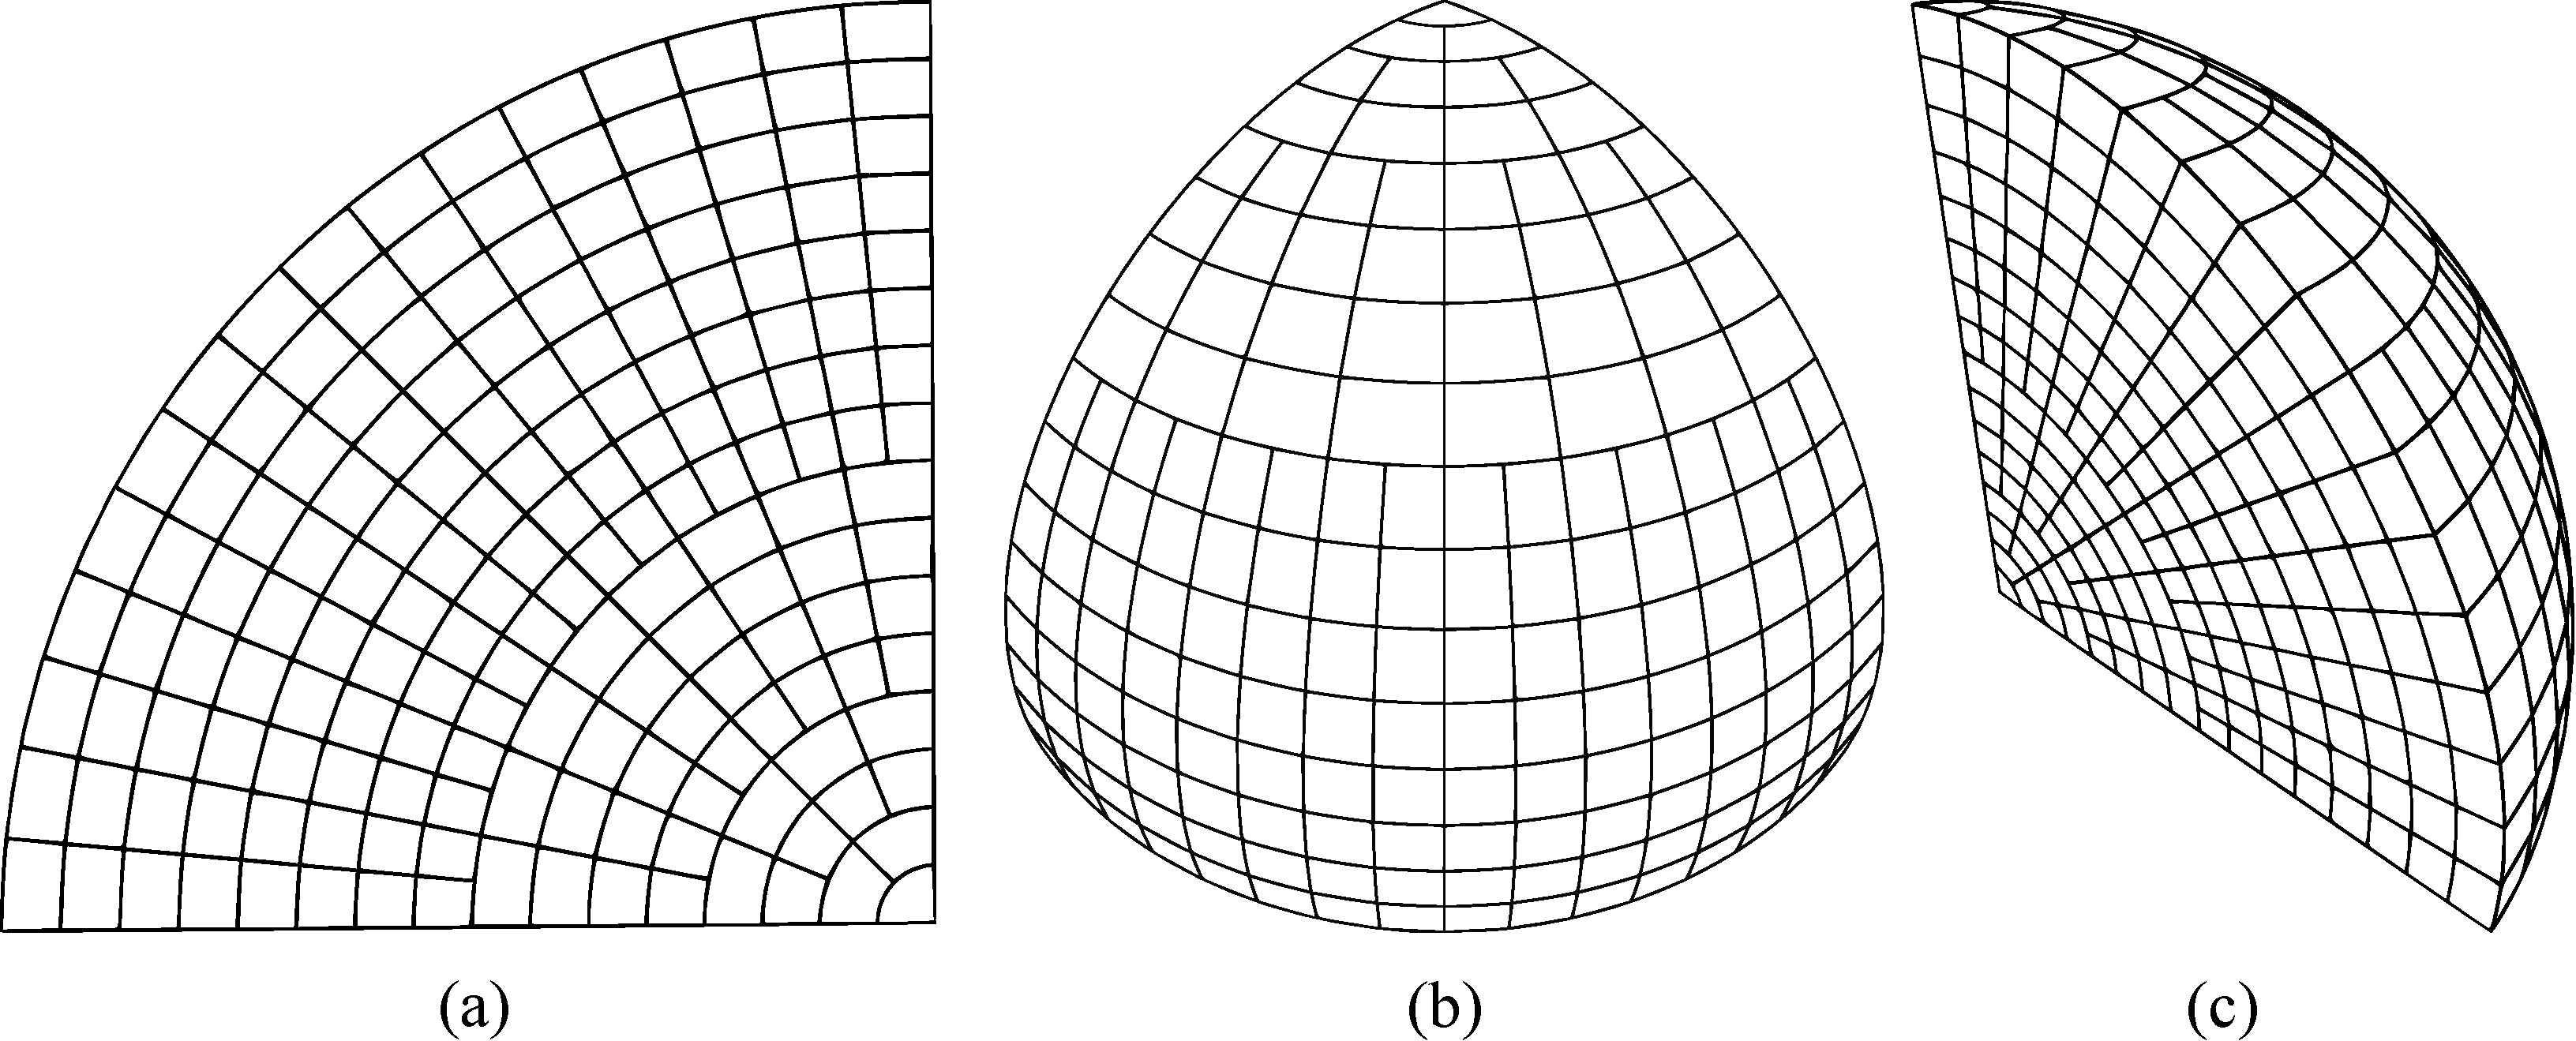
\includegraphics[width=\textwidth]{Fig2.pdf}
	\caption{One octant of an SDOG grid after four levels of subdivision viewed (a) from the side, (b) from the front, and (c) at an angle.
		Compared to a 3D LLG, cells are much more uniform in size and have much better compactness.
		Refer to Section~\ref{sec:results} for a detailed analysis of the volume preserving and compactness properties of SDOG}
	\label{fig:sdog}
\end{figure}


We first provide a brief explanation of SDOG construction and refinement as presented in~\cite{yu2009sdog}.
SDOG is an extension of the traditional octree to a spherical, as opposed to Euclidean, volume.
A sphere with twice the radius of the Earth is initially divided into eight equal octants via the equatorial plane and two perpendicular meridian planes.
These octants are taken to be the coarsest cells of the grid and are then subdivided to create more fine discretizations of the sphere.
An SDOG octant after four subdivisions can be seen in Figure~\ref{fig:sdog}.


\begin{figure}[tbp]
	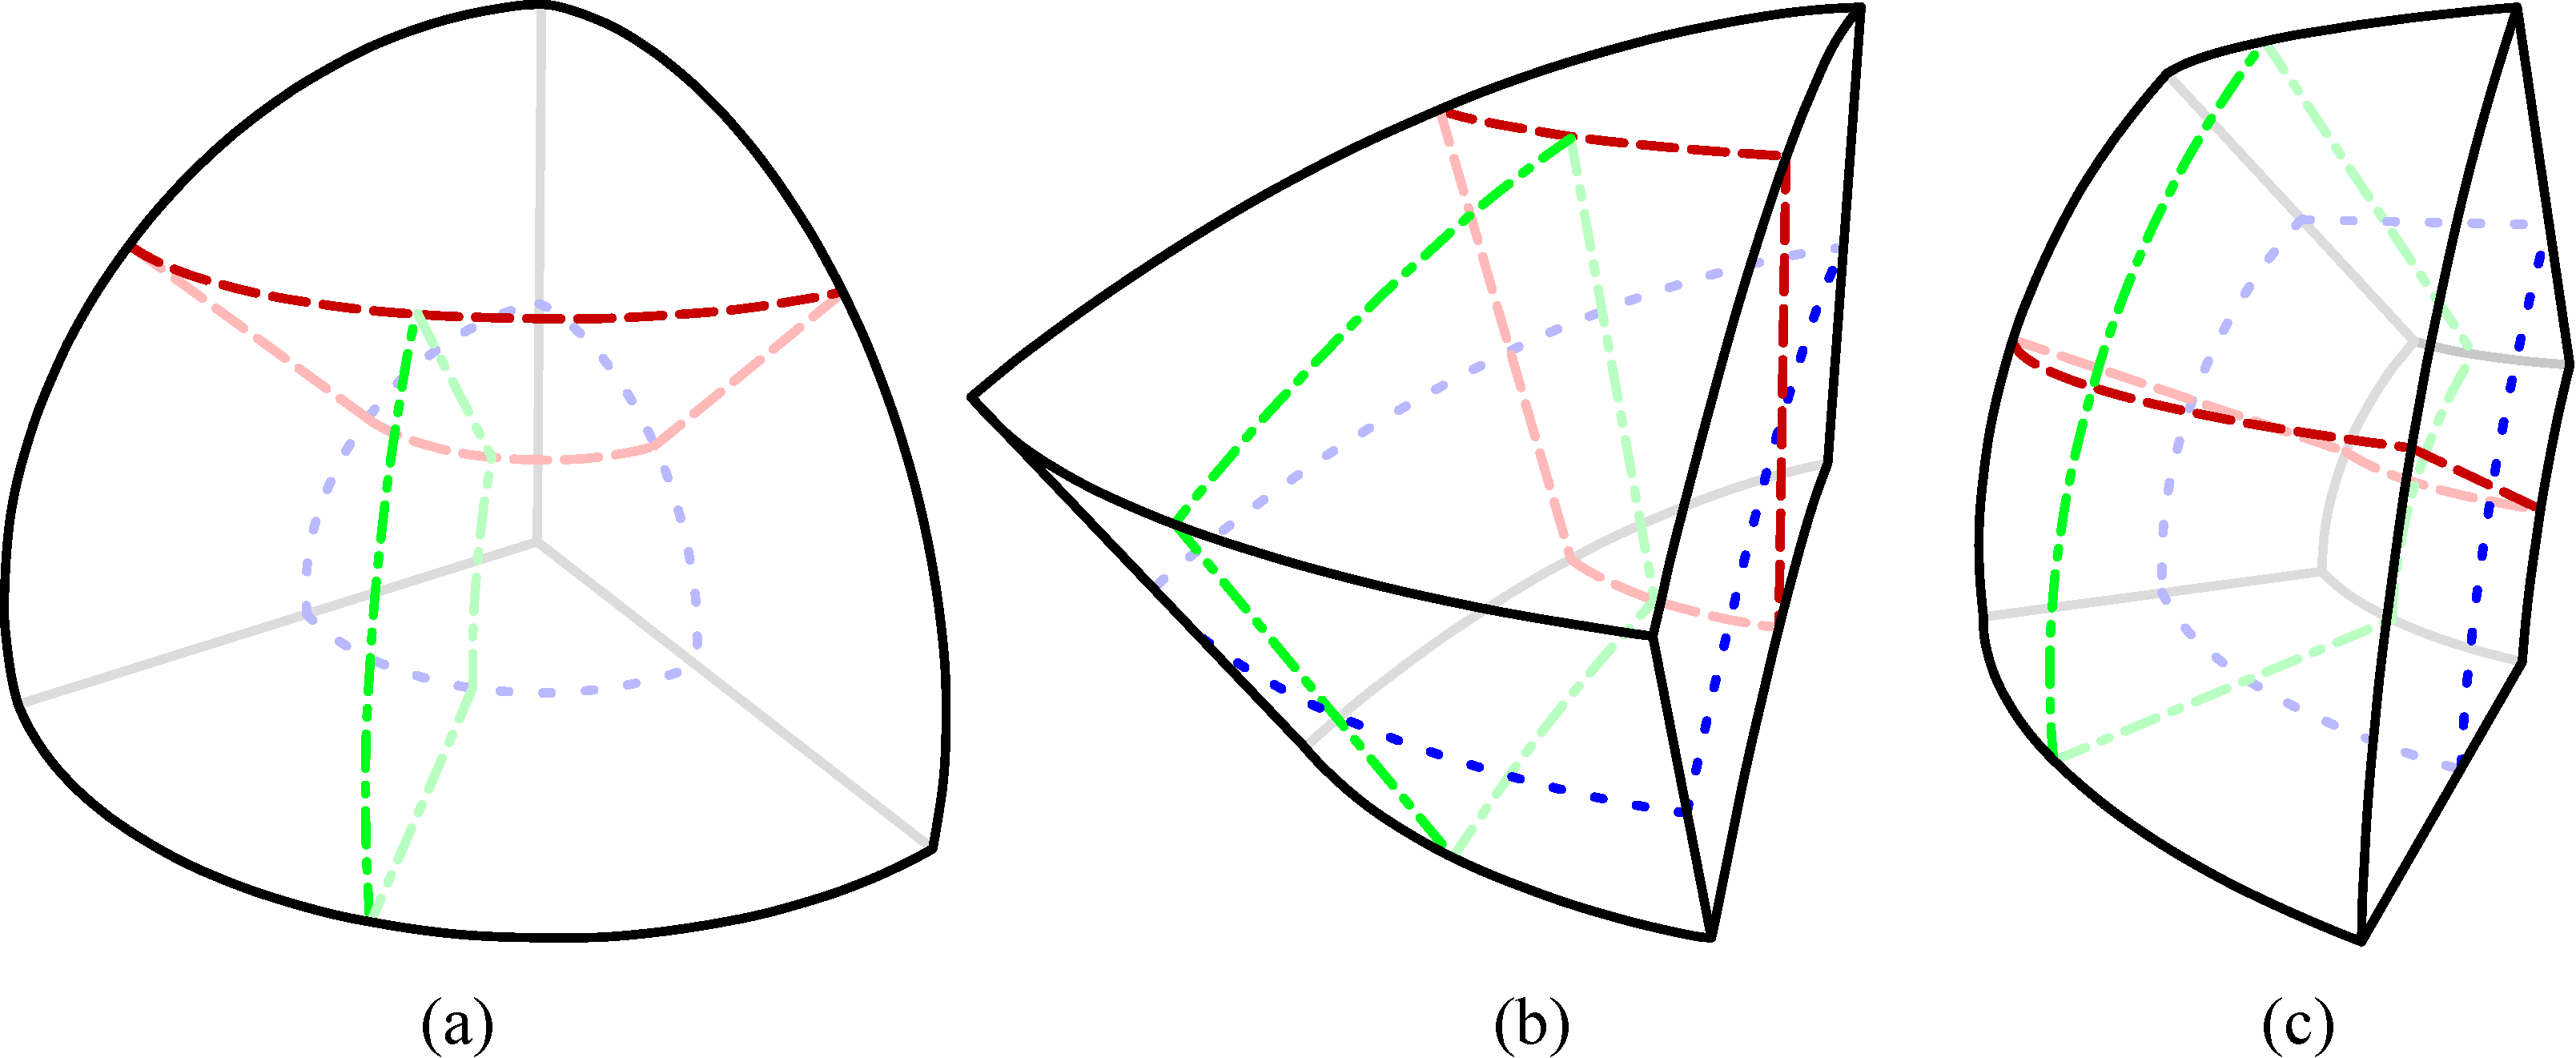
\includegraphics[width=\textwidth]{Fig3.pdf}
	\caption{Location and extent of splitting surfaces in SDOG subdivision for (a) SG cells, (b) LG cells, and (c) NG cells.
		Only NG cells have all three splitting surfaces fully subdivide the cell into eight children, and make up the majority of cells as the grid becomes more refined.
		Adapted from~\cite{yu2009sdog}}
	\label{fig:subRules}
\end{figure}


SDOG cells (including octants) are subdivided using the midpoint of each spherical coordinate: latitude, longitude, and radius.
These midpoints create splitting surfaces that can be used to split parent cells into smaller children cells.
To prevent the degeneration in cell compactness and size near the poles and centre of the sphere seen in 3D LLGs (Figure~\ref{fig:3dllg}), the extent of these splitting surfaces and the number of resulting children cells depends on the shape, or class, of cell that is being divided.
The splitting surfaces for each type of SDOG cell are shown in Figure~\ref{fig:subRules}.
We call a splitting surface symmetric if it creates the same number and type(s) of cells on both sides; otherwise we call it degenerate.


Cells that extend to the centre of the sphere and to one of the poles are referred to as Sphere-degenerated Grid (SG) cells (Figure~\ref{fig:subRules}a) and include the original eight octants.
For these cells, the longitudinal splitting surface does not extend beyond the latitudinal one in the direction towards the pole.
Additionally, neither the latitudinal nor longitudinal splitting surfaces extend beyond the radial one in the direction towards the centre of the sphere.
The result of this subdivision is four children cells: another SG cell, one Latitude-degenerated Grid (LG) cell, and two Normal Grid (NG) cells.
LG and NG cells are described below.
Only the longitudinal splitting surface for SG cells is symmetric.


LG cells (Figure~\ref{fig:subRules}b) are similar to SG ones, except that they only extend to one of the poles and not the centre of the sphere.
Therefore, the longitudinal splitting surface does not extend beyond the latitudinal one in the direction towards the pole.
This subdivision results in six children cells: two LG cells and four NG cells.
The longitudinal and radial splitting surfaces for LG cells are symmetric.


NG cells (Figure~\ref{fig:subRules}c) extend to neither the pole nor the centre of the sphere and make up the majority of SDOG cells.
These cells are fully subdivided into eight children NG cells and are the regular case for SDOG subdivision.
All splitting surfaces for NG cells are symmetric.


\subsection{SDOG Indexing} \label{sec:sdog-indexing}
In order to identify and distinguish the cells of a grid, there needs to be a method to assign a unique index to each cell.
A good indexing scheme will allow for efficient data insertion, retrieval, and manipulation via a set of queries.
Examples of some of these queries are: point to cell, which give the index of the cell containing a given point; index inversion, which calculates a cell's location and geometry from the index; neighbourhood queries; and in the case of a hierarchical grid, hierarchy traversal to find parent and children cells.


Due to the fact that SDOG subdivision is based on the midpoints of spherical coordinates, an indexing scheme that is efficient for many of the above operations can be easily developed.
At any subdivision level, $k$, each cell can be given an integer index in each spherical coordinate ranging from zero to $2^{k} - 1$.
To address the degenerate subdivision of certain cells, these integer indices are modified appropriately with divisions by powers of two, which can be done quickly with bit shift operations.
The integer indices can then be linearized by various methods, one good choice being a Z-order curve \cite{morton1966computer} as used in \cite{yu2009sdog}.
A more detailed description of degenerate Z-order indexing for SDOG grids, including algorithms for point to cell and index inversion operations, can be found in \cite{yu2009coding}.


\subsection{Number of SDOG Cells} \label{sec:sdog-numCells}
Being able to analyze the number of cells in the grid at each level of subdivision is useful not only for measuring volume preserving properties---such as quickly calculating the average cell volume---but also for analyzing the behavior of the grid as the level of subdivision increases.
This type of analysis will prove useful in informing decisions about how to modify subdivision to improve volume preservation.


Due to the degenerate nature of SDOG subdivision, calculating the number of cells in the grid is more complicated than a simple exponential formulation.
Despite this, we can use the above subdivision rules to derive recursive definitions for the number of cells in an SDOG grid (or a single octant) at a given level of subdivision.
Let $S(k)$, $L(k)$, $N(k)$, and $T(k)$ be the number of SG, LG, NG, and total cells of an SDOG octant at subdivision level $k$, respectively.
There is only ever one SG cell in an SDOG octant, so trivially
%
\begin{equation}
S(k) = 1.
\label{eq:sg-num}
\end{equation}
%
We know each LG cell produces two new LG cells, and that the SG cell produces one new LG cell.
From this we can say
\begin{equation*}
L(k) = 2L(k-1) + 1 \quad\text{and}\quad L(1) = 1.
\label{eq:lg-recursive}
\end{equation*}
%
Similarly, each NG cell produces eight new NG cells, each LG cell produces four, and the SG cell produces two.
Thus
\begin{equation*}
N(k) = 8N(k-1) + 4L(k-1) + 2 \quad\text{and}\quad N(1) = 2.
\label{eq:ng-recursive}
\end{equation*}
%
$L(k)$ is a linear non-homogeneous recurrence which can be solved with standard techniques \cite{bellman1963differential}.
Solving and substituting into $N(k)$ we get another linear non-homogeneous recurrence which can be solved similarly.
Finally, we get the closed forms:
%
\begin{equation}
L(k) = 2^{k} - 1,
\label{eq:lg-closed}
\end{equation}
%
\begin{equation}
N(k) = \frac{1}{21} \left( 7*2^{k} + 8^{k+1} + 6 \right) - 2^{k}, \quad\text{and}
\label{eq:ng-closed}
\end{equation}
%
\begin{equation}
T(k) = S(k) + L(k) + N(k) = \frac{1}{21} \left( 7*2^{k} + 8^{k+1} + 6 \right).
\label{eq:t-closed}
\end{equation}
%
As far as we are aware, these formulations have not been provided in any of the existing literature on SDOG.


\subsection{Geometry of SDOG Cells} \label{sec:sdog-geometry}
In order to measure the volume preservation properties of SDOG and its modifications, it is necessary to be able to measure the volume of individual cells in the grid.
Since each SDOG cell can be expressed as a range of each spherical coordinate (latitude $\phi$, longitude $\lambda$, and radius $r$), calculating the volume of an individual cell is a straightforward task.
Note that we use the geographic convention for spherical coordinates in this paper.
Let the subscripts $2$ and $1$ denote the maximum and minimum of a given spherical coordinate for an SDOG cell, then the volume is given by \cite{yu2009sdog}
%
\begin{equation}
V = \frac{1}{3} \left( \lambda_{2} - \lambda_{1} \right) \left(r_{2}^{3} - r_{1}^{3} \right) \left(\sin\phi_{2} - \sin\phi_{1} \right).
\label{eq:volume}
\end{equation}


In addition to the volume of a cell, surface area is another useful property to be able to measure.
Combined with the volume of cells, this allows us to measure the compactness of cells, which we use in Section \ref{sec:results} to help evaluate the consequences of our modifications.
From the fact that SDOG cells are subdivided using spherical coordinates, each face of a cell is a section of a simple geometric shape.
Faces created by radial splitting surfaces are spherical, with surface area given by
%
\begin{equation}
r^{2} \left( \lambda_{2} - \lambda_{1} \right) \left( \sin\phi_{2} - \sin\phi_{1} \right).
\end{equation}
%
Faces created by longitudinal splitting surfaces are the difference of two circular sectors, and have an area of
\begin{equation}
\frac{1}{2} \left( \phi_{2} - \phi_{1} \right) \left( r_{2}^{2} - r_{1}^{2} \right).
\end{equation}
%
Finally, faces created by latitudinal splitting surfaces lie on a cone, with a surface area of
\begin{equation}
\frac{1}{2} \cos\phi \left( \lambda_{2} - \lambda_{1} \right) \left( r_{2}^{2} - r_{1}^{2} \right).
\end{equation}


\section{Modified SDOG Subdivision} \label{sec:method}
%\subsection{Ideal Placement of Splitting Surfaces}
%\subsection{Blending Functions}

\begin{figure}[tbp]
	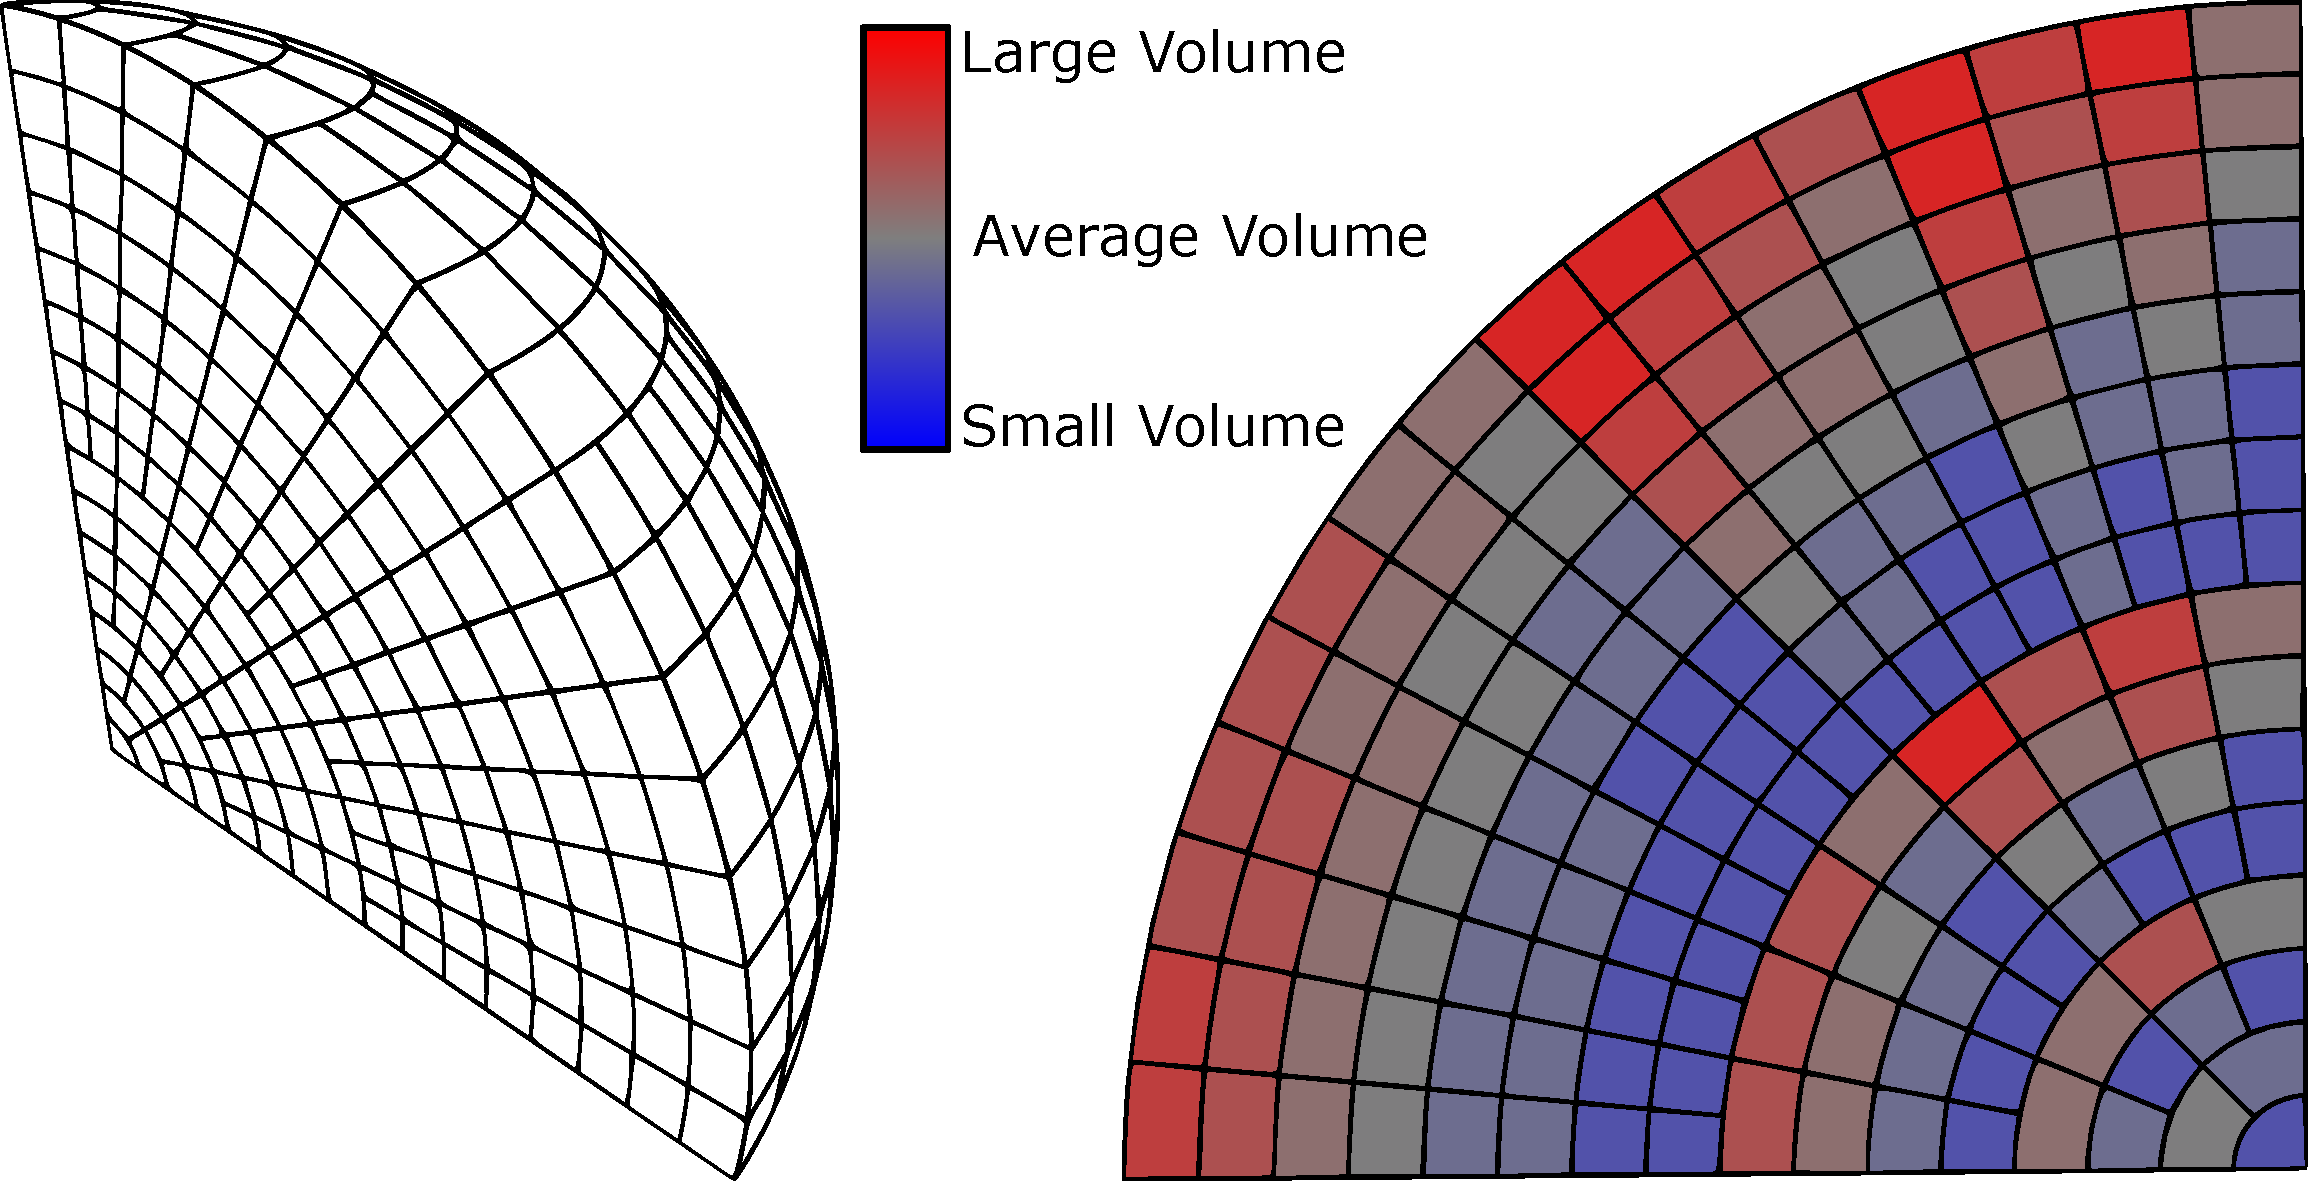
\includegraphics[width=0.85\textwidth]{Fig4.pdf}
	\caption{Distribution of cell volumes in an octant after four levels of conventional SDOG subdivision}
	\label{fig:sdog-vol}
\end{figure}


The main goal of this work is to modify SDOG in such a way as to improve volume preservation while minimizing the impact on other desired properties of the grid.
To aid in this task, we have developed a visualization framework for displaying and modifying SDOG grids.
This framework allows for changes to subdivision to be quickly implemented and allows visual analysis of said modifications.
All of the figures in the paper (except for the charts) were created using the output of this framework.
As an example and a baseline, the distribution of cell volumes in a conventional SDOG grid is visualized in Figure~\ref{fig:sdog-vol}.


As previously discussed, in conventional SDOG subdivision the location of the different splitting surfaces is always chosen to be at the midpoint of the respective spherical coordinate; we question if this should always be the case.
For an octree in Euclidean space this type of subdivision is desirable, as it generates children cells of identical size and shape.
In spherical space, however, this property does not transfer.
Using midpoints to subdivide cells makes for a simple subdivision scheme, but it makes no guarantees about the shape or size of the resulting children cells.


\begin{figure}[tbp]
	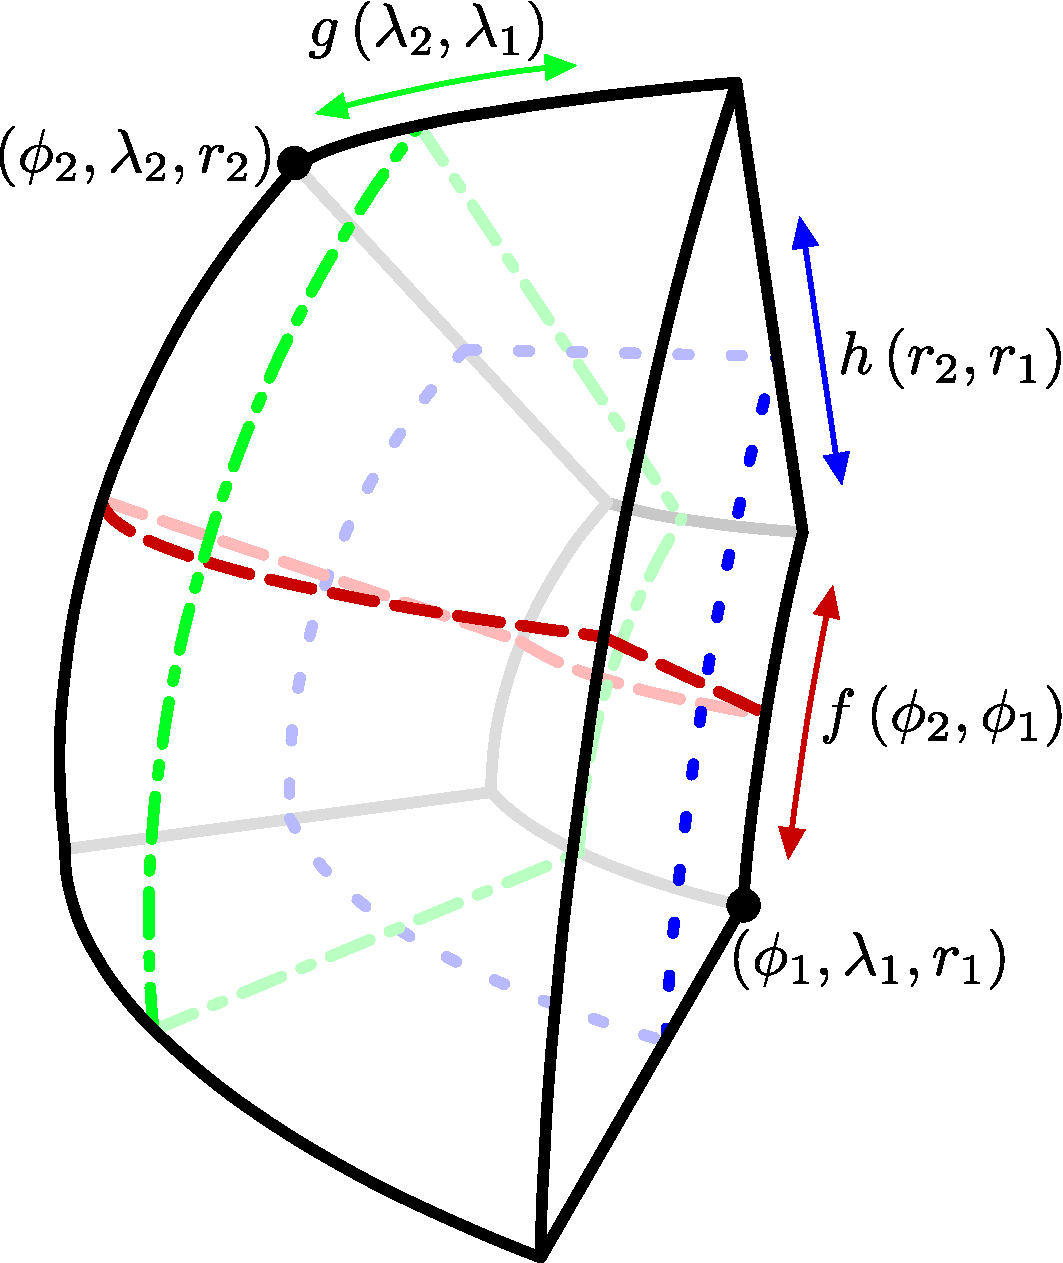
\includegraphics[width=0.5\textwidth]{Fig5.pdf}
	\caption{Each SDGO cell can be expressed as a range in each spherical coordinate, and the location of the splitting surface for each spherical coordinate can be expressed as a function of the maximum and minimum of the respective range.
		Here we show only an NG cell, however the same applies to SG and LG cells.
		The functions $f$, $g$, and $h$ serve as placeholders for any valid function that results in the output being strictly between the two inputs}
	\label{fig:functions}
\end{figure}


By allowing the location of the splitting surfaces to be adjusted, we can modify the shape and size of children cells and as a result affect the volume preservation, compactness, and other properties of the grid.
Let $c_{s}$ be the location of the splitting surface, where $c$ is one of $\left\lbrace \phi, \lambda, r \right\rbrace$, then one way to express the location of the splitting surfaces used for subdivision is as a convex combination of maximum and minimum values
%
\begin{equation} \label{eq:convex}
c_{s} = \alpha c_{2} + \left( 1-\alpha \right) c_{1}, \quad \alpha \in \left( 0, 1 \right),
\end{equation}
%
where we call $\alpha$ the splitting factor.
Conventional SDOG used midpoints (i.e.
$\alpha = \frac{1}{2}$) for each spherical coordinate when subdividing, regardless of cell type.
While a convex combination is the most straightforward, any function of the maximum and minimum such that the result is strictly between the two is a valid method for determining the location of the splitting surfaces (Figure~\ref{fig:functions}).
Thus, the location of splitting surfaces can be modified by changing this function, either by using a different value of $\alpha$, or by using a different function altogether.
Furthermore, the function used can be different for each cell type and spherical coordinate.


A useful function for improving volume preservation is one that results in one of the new ranges having a specific percentage of the volume of the original range.
We start with the radial splitting surface.
Referring to Eq.
(\ref{eq:volume}), let $p \in (0,1)$ be the percentage we wish for the lower range to have, then
%
\begin{equation*}
p \left( r_{2}^{3} - r_{1}^{3} \right) = r_{s}^{3} - r_{1}^{3}
\end{equation*}
%
\begin{equation*}
p r_{2}^{3} - p r_{1}^{3} = r_{s}^{3} - r_{1}^{3}
\end{equation*}
%
\begin{equation*}
r_{s}^{3} = p r_{2}^{3} + r_{1}^{3} - p r_{1}^{3}
\end{equation*}
%
\begin{equation*}
r_{s}^{3} = p r_{2}^{3} + \left( 1 - p \right) r_{1}^{3}
\end{equation*}
%
\begin{equation} \label{eq:radVol}
r_{s} = \sqrt[3]{ p r_{2}^{3} + \left( 1 - p \right) r_{1}^{3} }.
\end{equation}
%
The derivations for the latitudinal and longitudinal splitting surfaces follow the same, with results
%
\begin{equation} \label{eq:latVol}
\phi_{s} = \sin^{-1} \left( p \sin\phi_{2} + \left( 1 - p \right) \sin\phi_{1} \right), \quad\text{and}
\end{equation}
%
\begin{equation} \label{eq:longVol}
\lambda_{s} = p \lambda_{2} + \left( 1 - p \right) \lambda_{1}.
\end{equation}


The question then becomes which splitting surfaces can be modified, and in which ways, in order to improve the volume preservation of the grid.
We first look at which splitting surfaces should \textit{not} be modified.
From Eq.~(\ref{eq:longVol}) it is clear a longitudinal splitting surface at the midpoint will always split a cell exactly in half, and therefore since all longitudinal splitting surfaces are symmetric, they should not be changed.


\begin{figure}[tbp]
	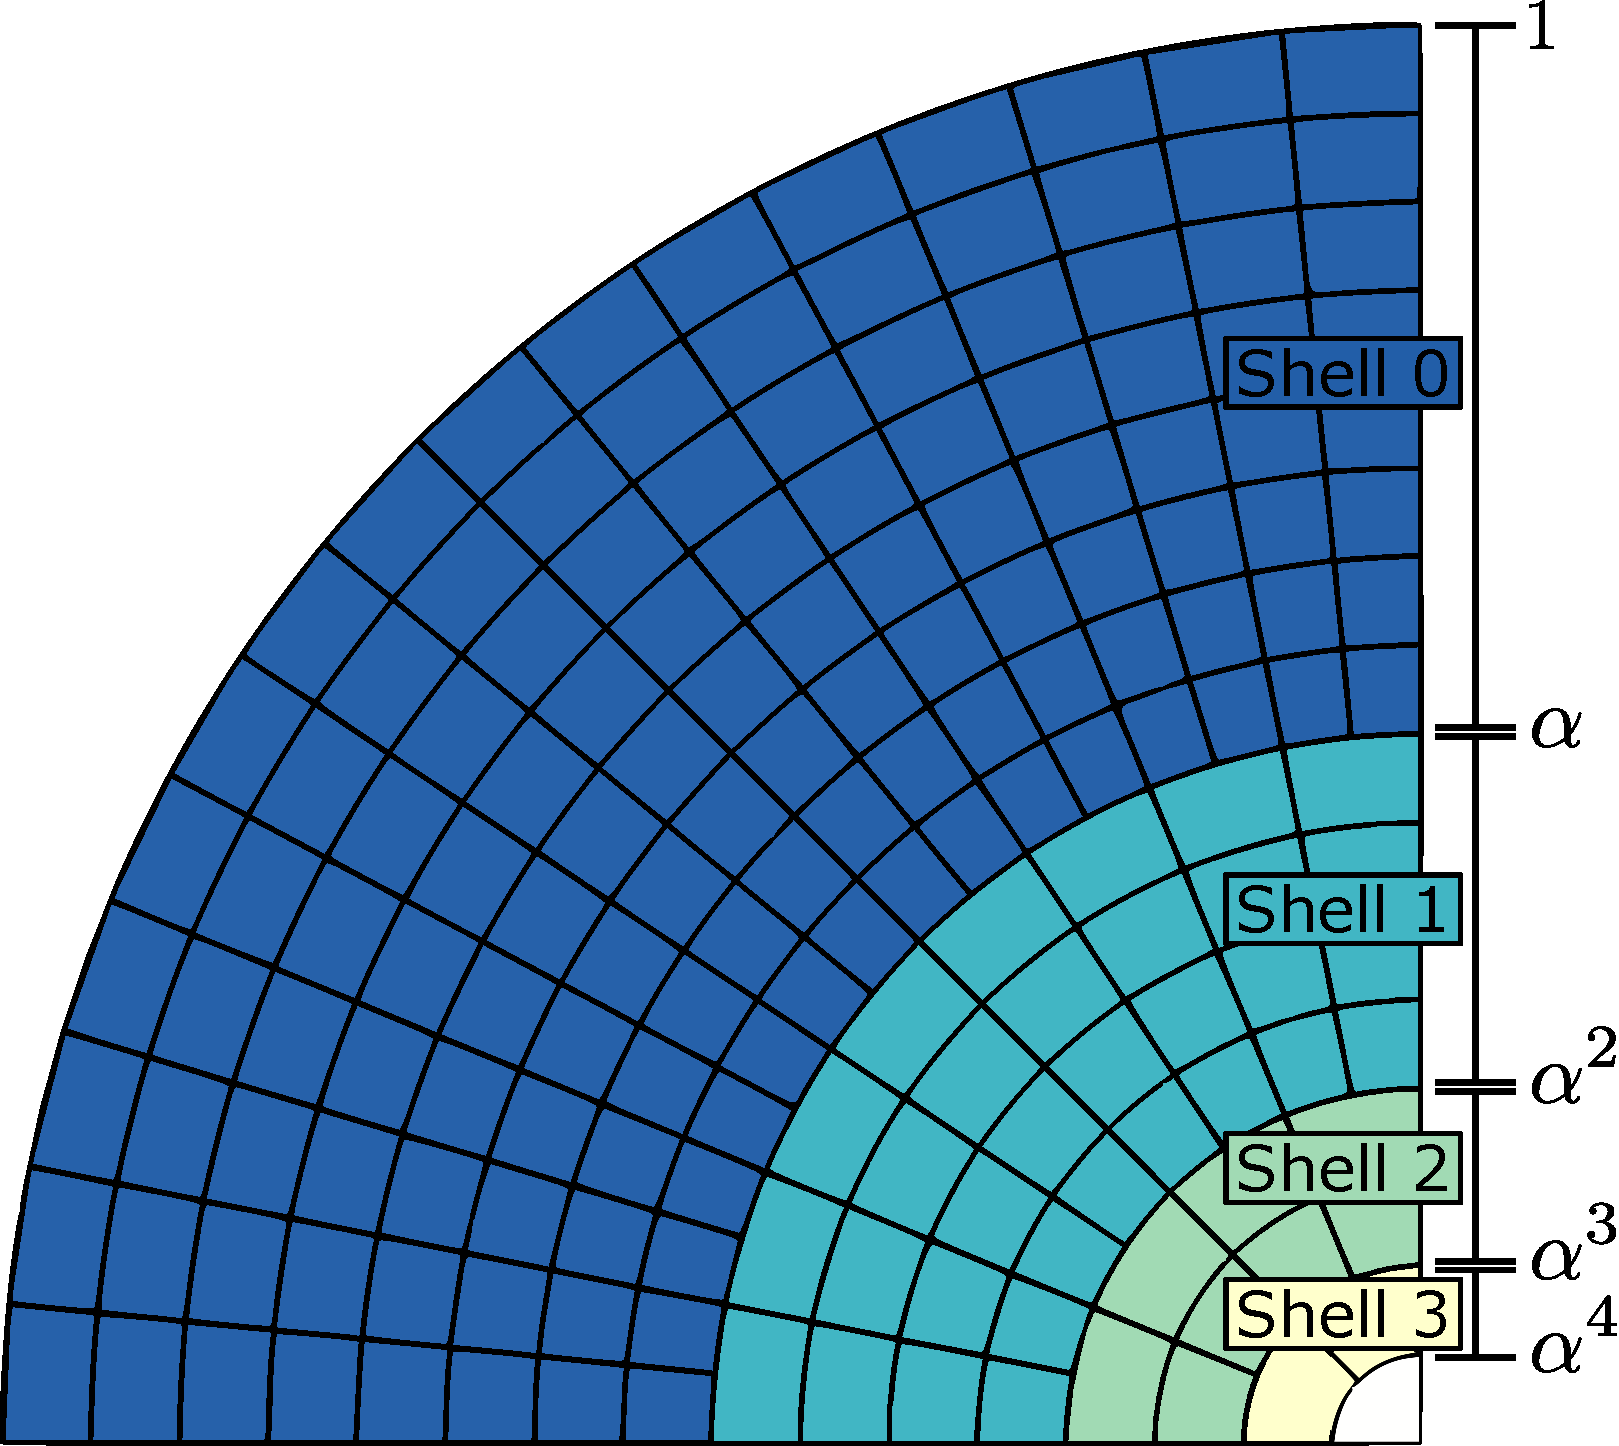
\includegraphics[width=0.6\textwidth]{Fig6.pdf}
	\caption{Spherical shells created by the radial splitting surfaces of SG cells.
		At $k$ levels of subdivision there are $k$ shells and one inner SG cell.
		These shells are similar and should have volume proportional to the number of cells they contain}
	\label{fig:sg-rad-splits}
\end{figure}


Less trivially, the radial splitting surface for SG cells should also be left at the midpoint.
Referring to Figure~\ref{fig:sg-rad-splits}, we can see that the radial splitting surfaces for SG cells separate the grid into spherical shells.
Shell $n$ has a volume proportional to
%
\begin{equation}
\alpha^{3n} - \alpha^{3 \left( n + 1 \right)},
\end{equation}
%
then the ratio of the volume between shell $n+1$ and $n$ is
%
\begin{equation}
\frac{ \alpha^{3 \left(n + 1 \right)} - \alpha^{3\left( n + 2 \right)} }{ \alpha^{3n} - \alpha^{3 \left( n + 1 \right)} } = \frac{ \alpha^{3} \alpha^{3n} \left( 1 - \alpha^{3} \right) }{ \alpha^{3n} \left( 1 - \alpha^{3} \right) } = \alpha^{3}.
\end{equation}
%
From the self similar nature of SDOG subdivision, we know that the cells in shell $n$ are simply the cells of shell $n+1$ subdivided once.
We also know that in the limit, an SDOG grid at one level higher of subdivision will have eight times as many cells as the previous resolution $\left( \lim_{k \to \infty} \frac{ T(k+1) }{ T(k) }  = 8 \right)$.
Therefore, in order for cells in the grid to be close to equal volume, it must be that shell $n+1$ has one eighth the volume of shell $n$ (since it will have one eighth the number of cells), which occurs exactly when $\alpha = \frac{1}{2}$.


This leaves five possible splitting surfaces that can be modified: the radial splitting surface for LG and NG cells, and the latitudinal splitting surface for SG, LG, and NG cells.
An important decision then is whether to use convex combinations to calculate the location of these surfaces (Eq.~(\ref{eq:convex})), or to use the functions parameterized by the ratio of volumes (Eq.~(\ref{eq:radVol}) and (\ref{eq:latVol})).
This is akin to a stationary subdivision scheme in comparison to a non-stationary one.
A stationary scheme will maintain the simplicity of subdivision, however, offers less overall ability to improve volume preservation.
Because of this, we provide both a stationary and non-stationary set of modifications.


\subsection{Stationary Subdivision} \label{sec:method-stationary}
By constraining splitting surfaces to be calculated via convex combinations, there are more restrictions on which splitting surfaces should be modified.
An interesting property of SDOG subdivision is that if a cell subdivides symmetrically in a given spherical dimension, all children of that cell also subdivide symmetrically in that dimension.
Thus, symmetric splitting surfaces result in non-degenerate binary (in the given dimension) subdivision at all further levels of subdivision, and it becomes clear that using any other value than the midpoint results in divergence as the level of subdivision gets large.
Therefore, all symmetric splitting surfaces should be left at the midpoint, which leaves only the latitudinal splitting surface for SG and LG cells to be modified.
We use $\alpha_{\phi}^{SG}$ and $\alpha_{\phi}^{LG}$ to refer to the splitting factors used for calculating the location of these surfaces.


\begin{figure}[tbp]
	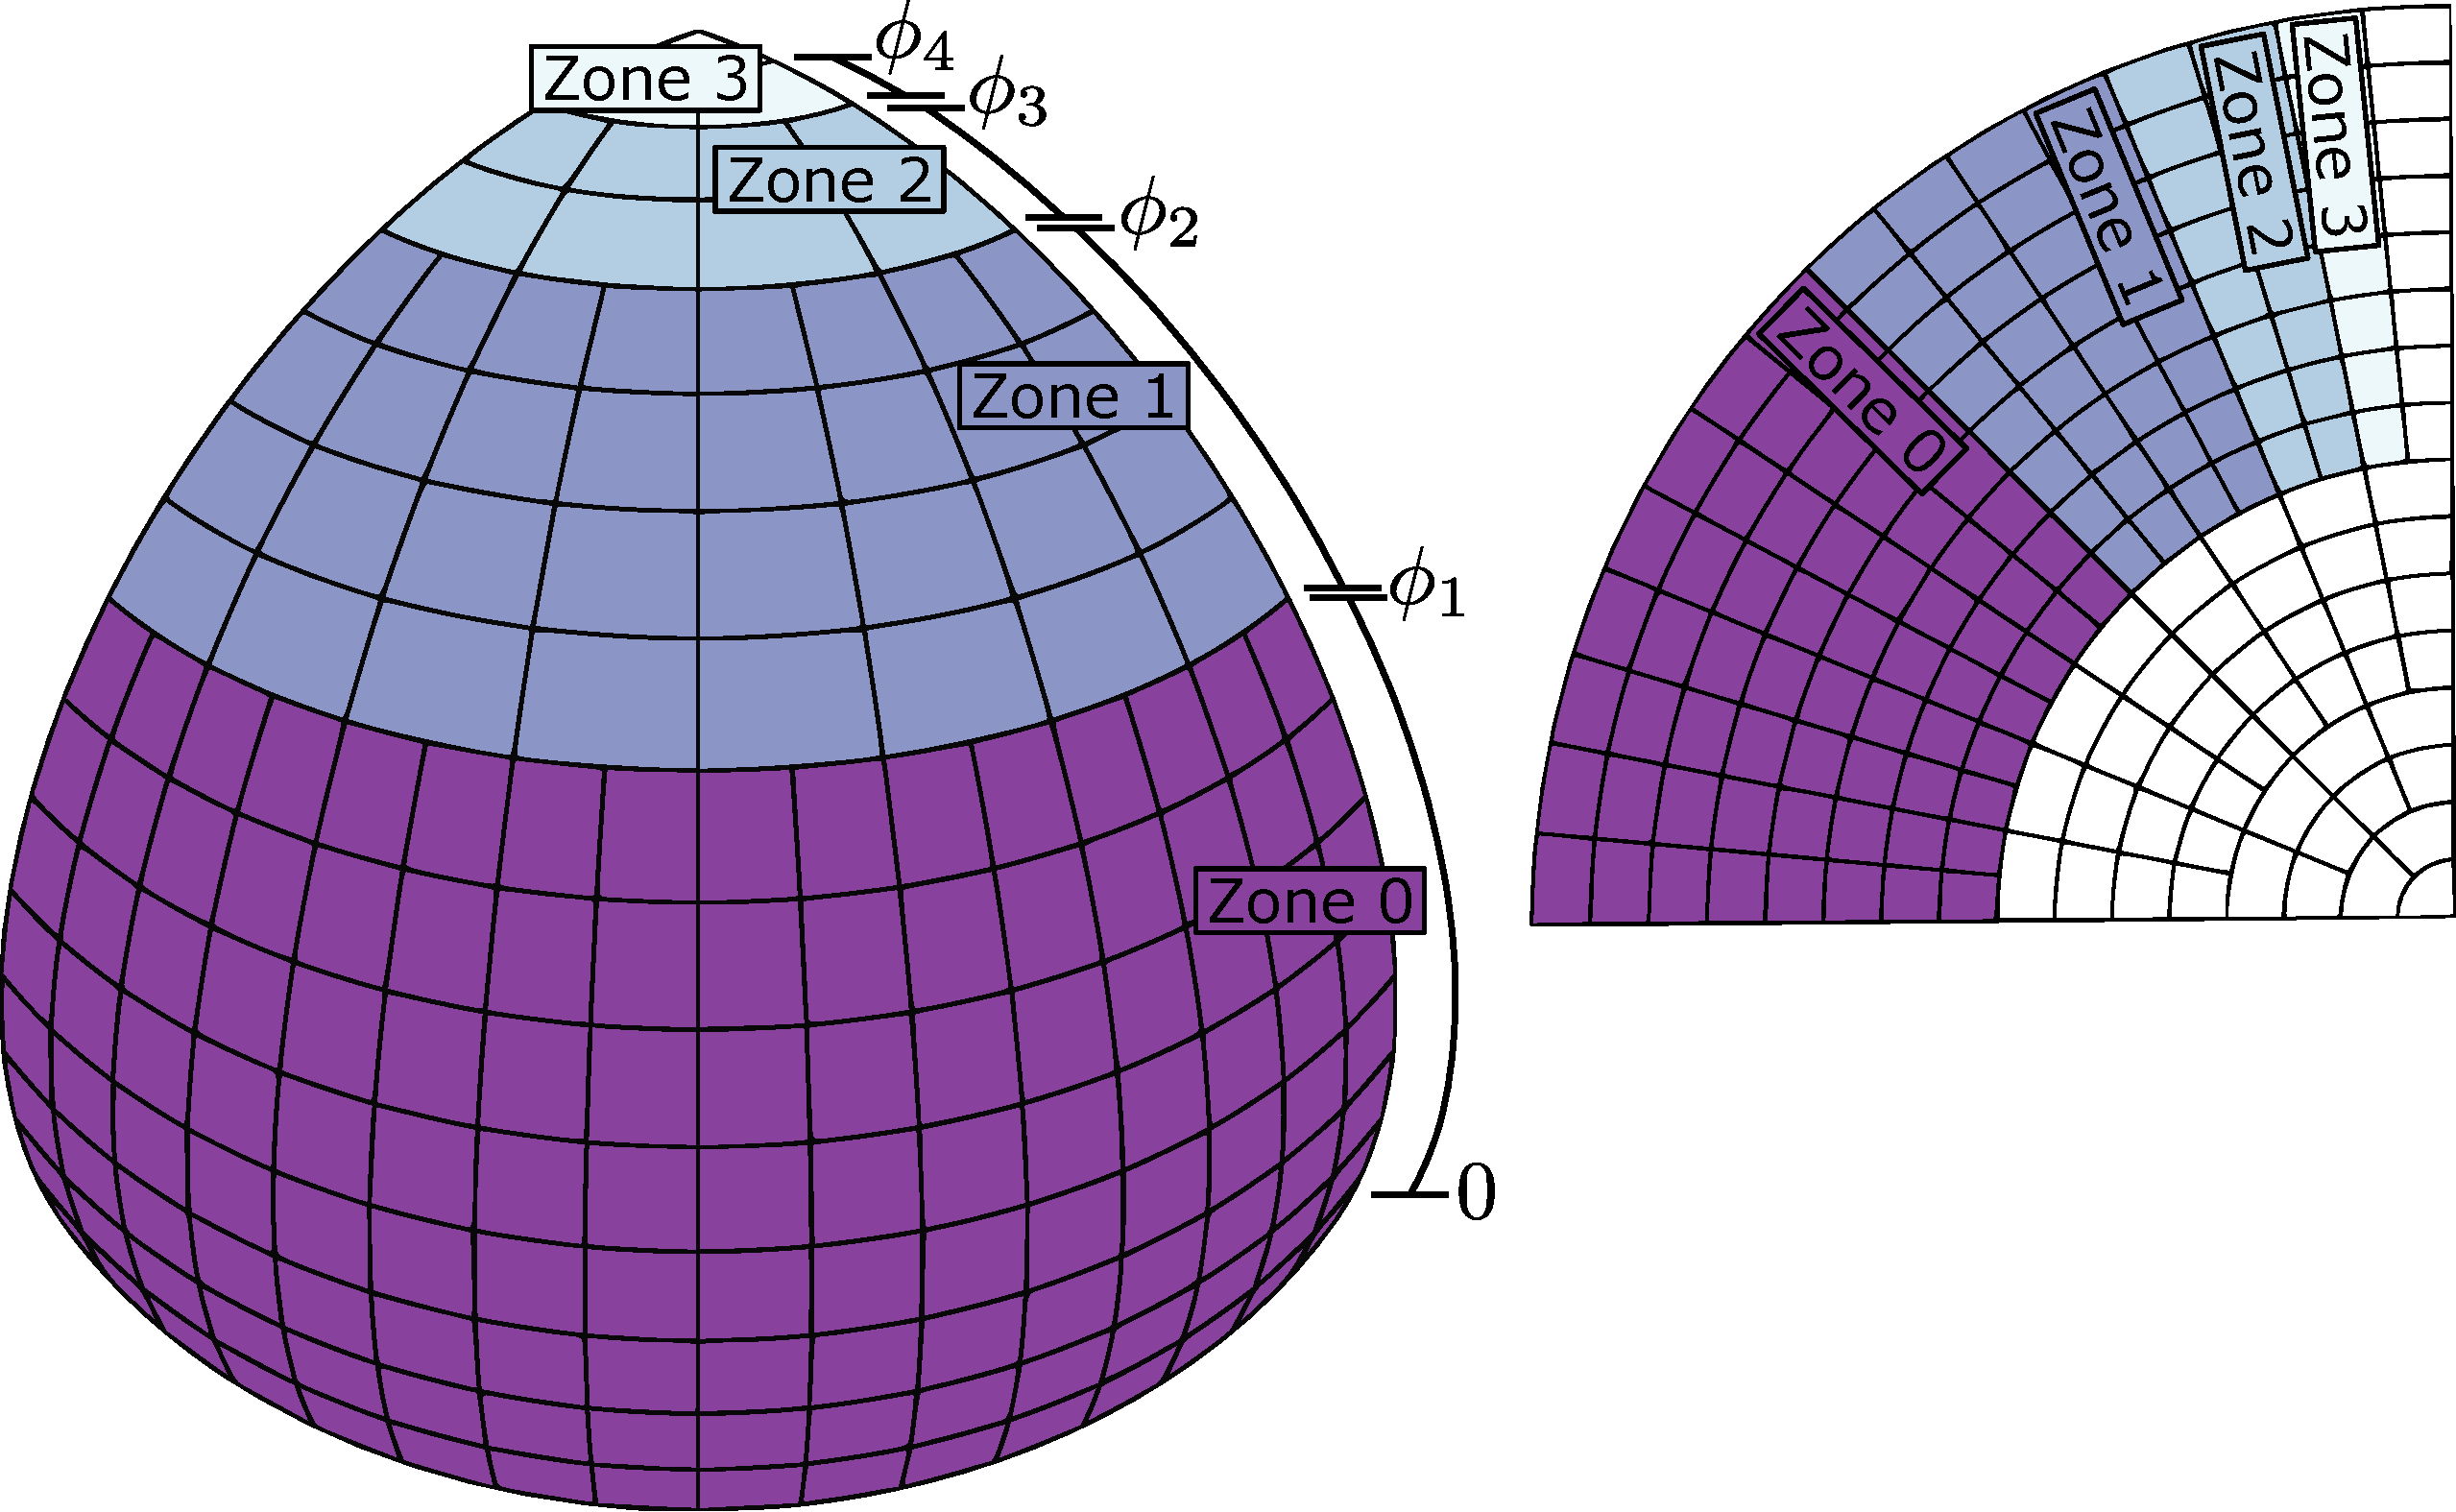
\includegraphics[width=0.9859\textwidth]{Fig7.pdf}
	\caption{Spherical zones created by the latitudinal splitting surfaces of SG and LG cells.
		At $k$ levels of subdivision there are $k$ zones and one upper stack of LG cells in the outer most shell.
		Each successively smaller shell has one fewer zones, until reaching the innermost SG cell.
		Zones in the same shell are not exactly similar, but are regular and should have volume proportional to the number of cells they contain}
	\label{fig:lat-splits}
\end{figure}


We first performed a simple search on the possible values of these splitting factors to see if it was possible to improve the volume preservation.
We found that volume preservation could be improved by certain values of $\alpha_{\phi}^{SG}$, however, it was always the case that $\alpha_{\phi}^{LG}$ was best left equal to one half.
To understand why this is the case, we look at where the ideal placements for these splitting surfaces would be if not constrained by convex combinations.
Notice that these two latitudinal splitting surfaces have a similar effect as the radial splitting surface for SG cells.
Referring now to Figure~\ref{fig:lat-splits}, we see that these splitting surfaces further divide the spherical shells into spherical zones.
Additionally, each zone is comprised entirely of NG cells.
From this fact we conclude that zone $n$ has exactly four times as many cells as zone $n+1$, and thus in the ideal case would have exactly four times the volume as well.
We can use Eq.~(\ref{eq:latVol}) to find these ideal locations using the proper value for $p$.
Zone $n$ has a percentage $\left( 1 - p \right)^{n} p$ of the initial volume of the octant, then setting the ratio between zone $n+1$ and $n$ to be equal to $\frac{1}{4}$ gives us $p = \frac{3}{4}$, and finally
%
\begin{equation} \label{eq:idealLat}
\phi_{s} = \sin^{-1} \left( \frac{3}{4} \sin\phi_{2} + \frac{1}{4} \sin\phi_{1} \right).
\end{equation}


From here, we can now see why the latitudinal splitting surfaces for LG cells should remain at the midpoint.
As $\phi_{1}$ approaches $\pm \frac{\pi}{2}$, this function is closely approximated by a convex combination with a factor of one half (see Appendix~\ref{app:lat}).
Thus, as the level of subdivision gets large, using $\alpha_{\phi}^{LG} = \frac{1}{2}$ approaches the ideal placement for the splitting surfaces, and thus is the ideal factor to use for a convex combination.


\begin{figure}[tbp]
	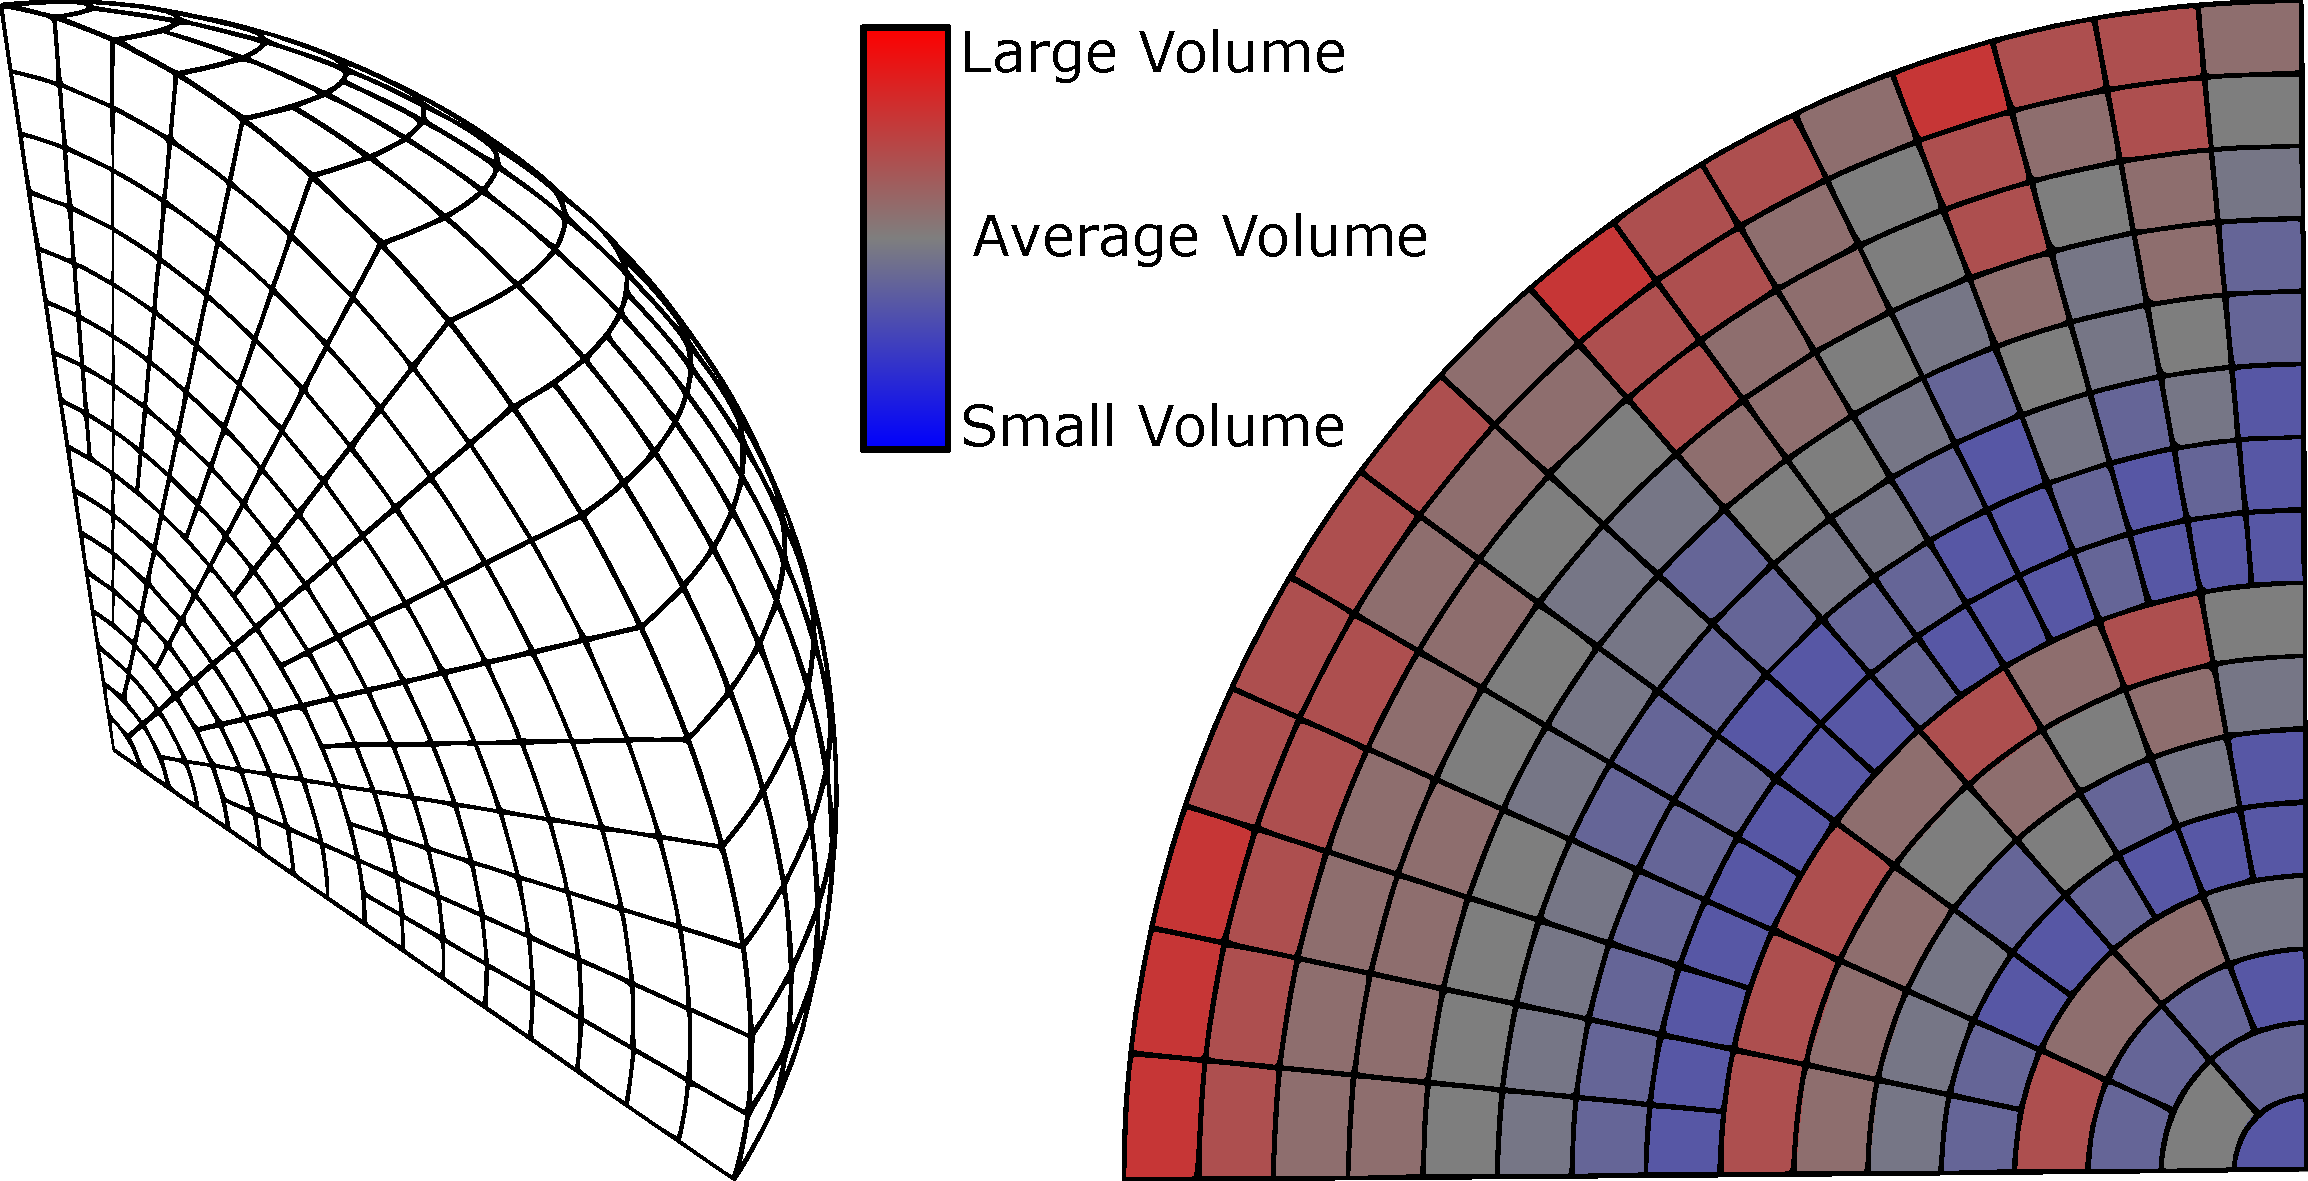
\includegraphics[width=0.85\textwidth]{Fig8.pdf}
	\caption{Results of the stationary scheme after four levels of subdivision using $\alpha_{\phi}^{SG} \approx 0.54$.
		Since only one type of splitting surface has been modified, the results are similar to that of conventional SDOG}
	\label{fig:stationary}
\end{figure}


We can also use this formulation to find the theoretical ideal placement for the latitudinal splitting surface of SG cells.
SG cells always have a minimum latitude of zero and a maximum of $\pm \frac{\pi}{2}$, thus Eq.~(\ref{eq:idealLat}) will always evaluate to plus or minus the same value.
Substituting back into Eq.~(\ref{eq:convex}) we get
%
\begin{equation} \label{eq:latValue}
\alpha_{\phi}^{SG} = \frac{ \sin^{-1} \left( \pm \frac{3}{4} \right) }{ \pm \frac{\pi}{2} } \approx 0.53989.
\end{equation}
%
The grid resulting from using this value can be seen in Figure~\ref{fig:stationary}.
Interestingly, our initial search also found $\alpha_{\phi}^{SG} = 0.57$ to perform well, even resulting in a slightly lower maximum difference in cell volumes than the theoretical ideal.
These findings are not necessarily in conflict, however, as the theoretical ideal results in much less variation in the volume of cells.
We compare these two schemes more closely in Section \ref{sec:results}.


\subsection{Non-Stationary Subdivision} \label{sec:method-nonStationary}
By not limiting splitting surfaces to be calculated using convex combinations, we are allowed much more control over subdivision and the resulting properties.
Using Eq~(\ref{eq:radVol}) and (\ref{eq:latVol}) to calculate the modifiable splitting surfaces, all that is needed is to determine the ideal value of $p$ for the different splitting surfaces and cell types.
We have already done this for the latitudinal splitting surfaces of SG and LG cells in Section \ref{sec:method-stationary} with Eq.~(\ref{eq:idealLat}).
Therefore, all that is left is the radial splitting surfaces for LG and NG cells, and the latitudinal one for NG cells.
However, since all of these remaining splitting surfaces are symmetric, we simply require that the volume on each side of these splitting surfaces be equal.
In other words, we can simply set $p = \frac{1}{2}$ for these remaining splitting surfaces.


\begin{figure}[tbp]
	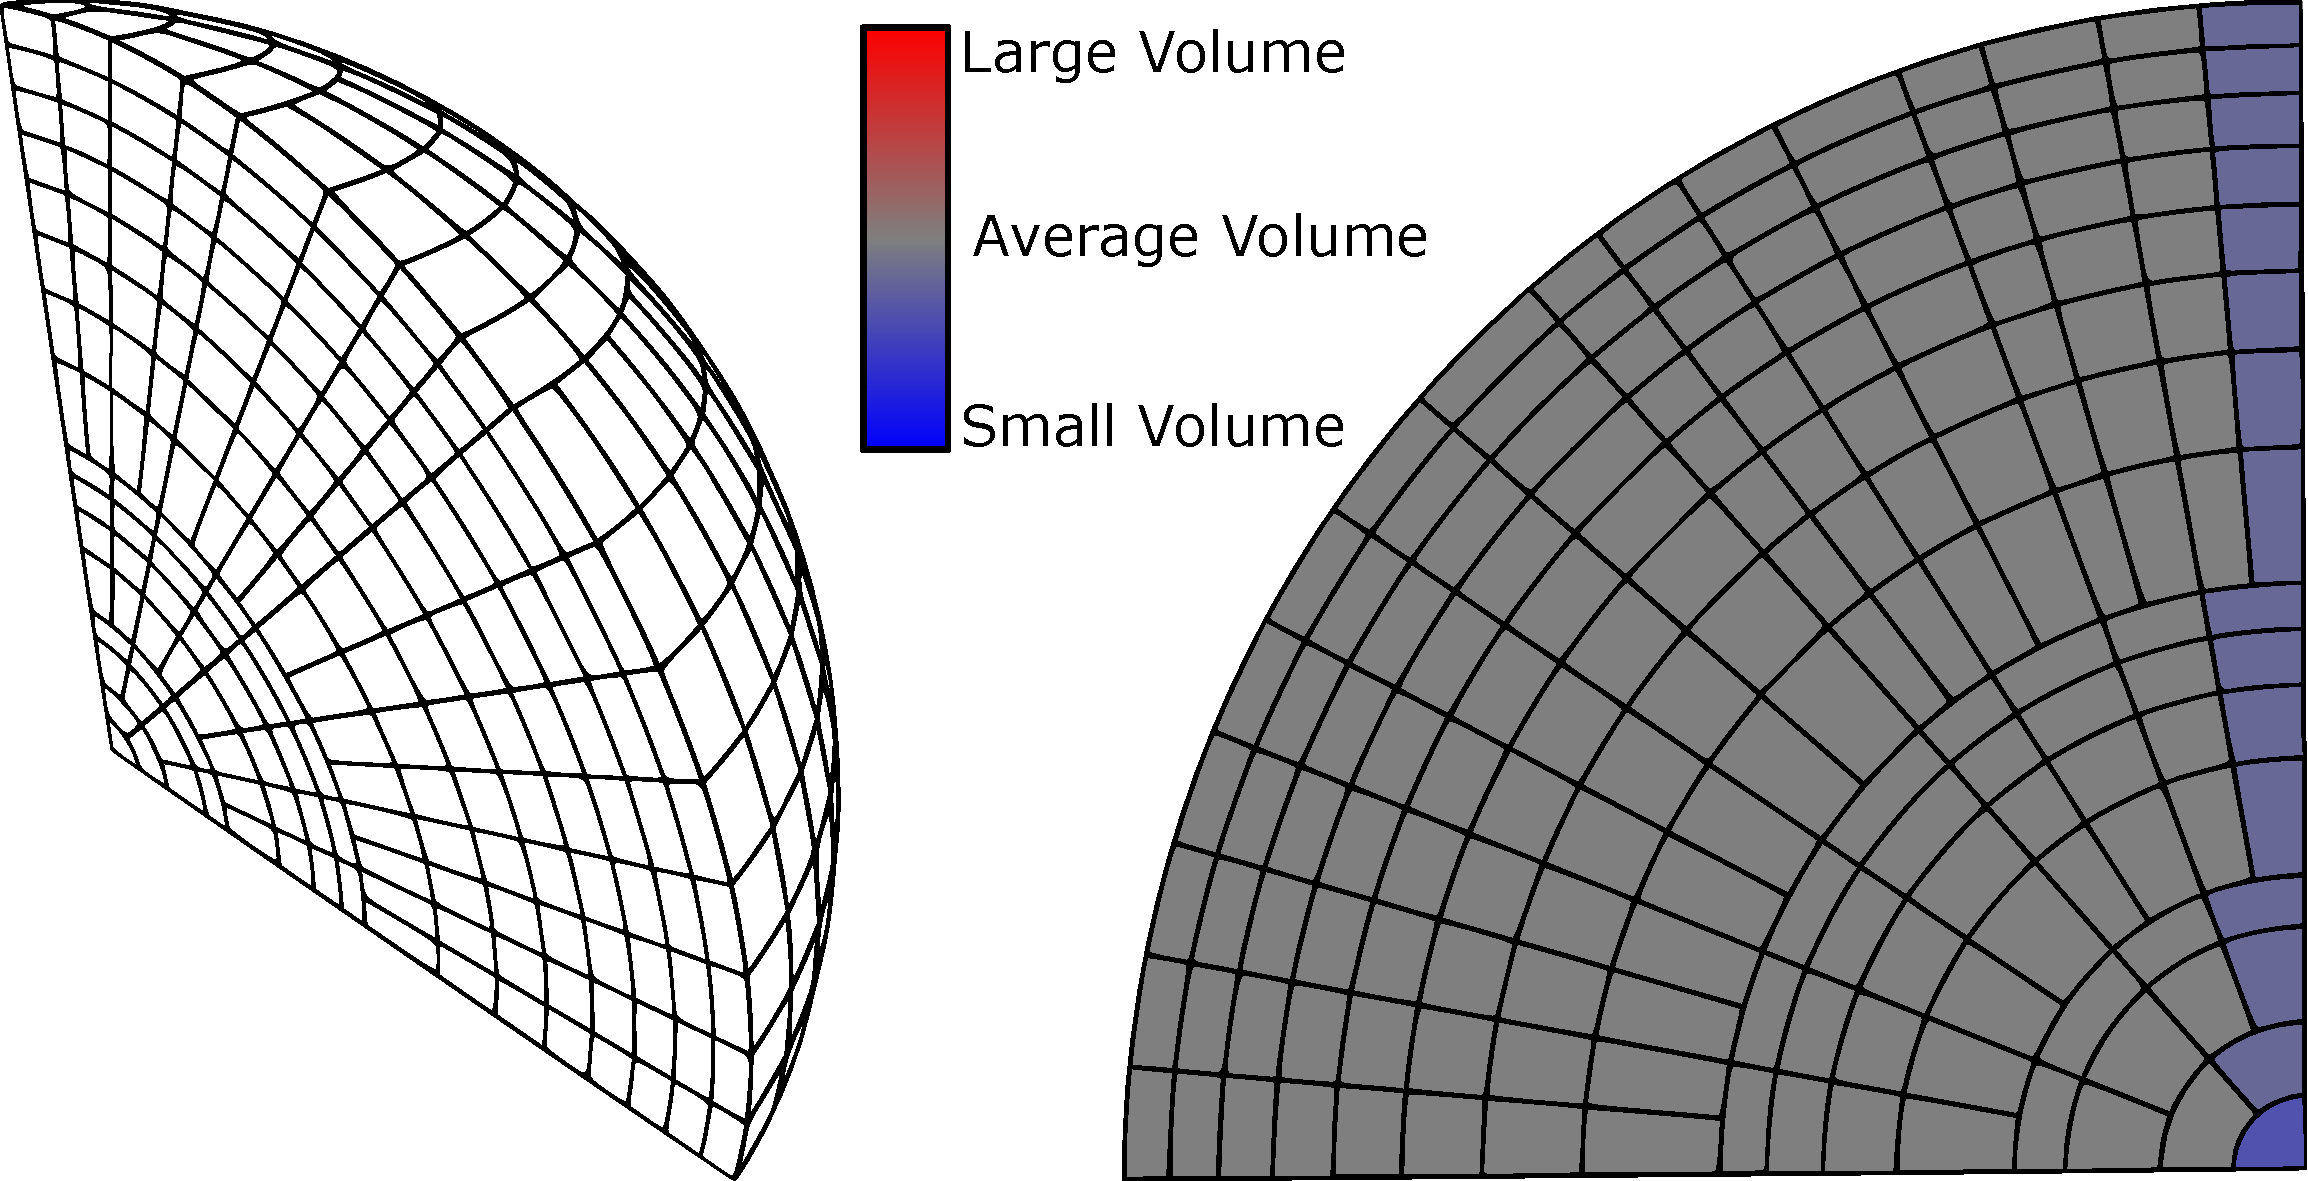
\includegraphics[width=0.85\textwidth]{Fig9.pdf}
	\caption{Results of the non-stationary scheme after four levels of subdivision using $\beta = 1$.
		All NG cells have exactly the same volume, with the LG and SG cells having a lower volume.
		Notice how the resulting NG cells are stretched and squashed in order to ensure they all have equal volume}
	\label{fig:perfect}
\end{figure}


\begin{figure}[tbp]
	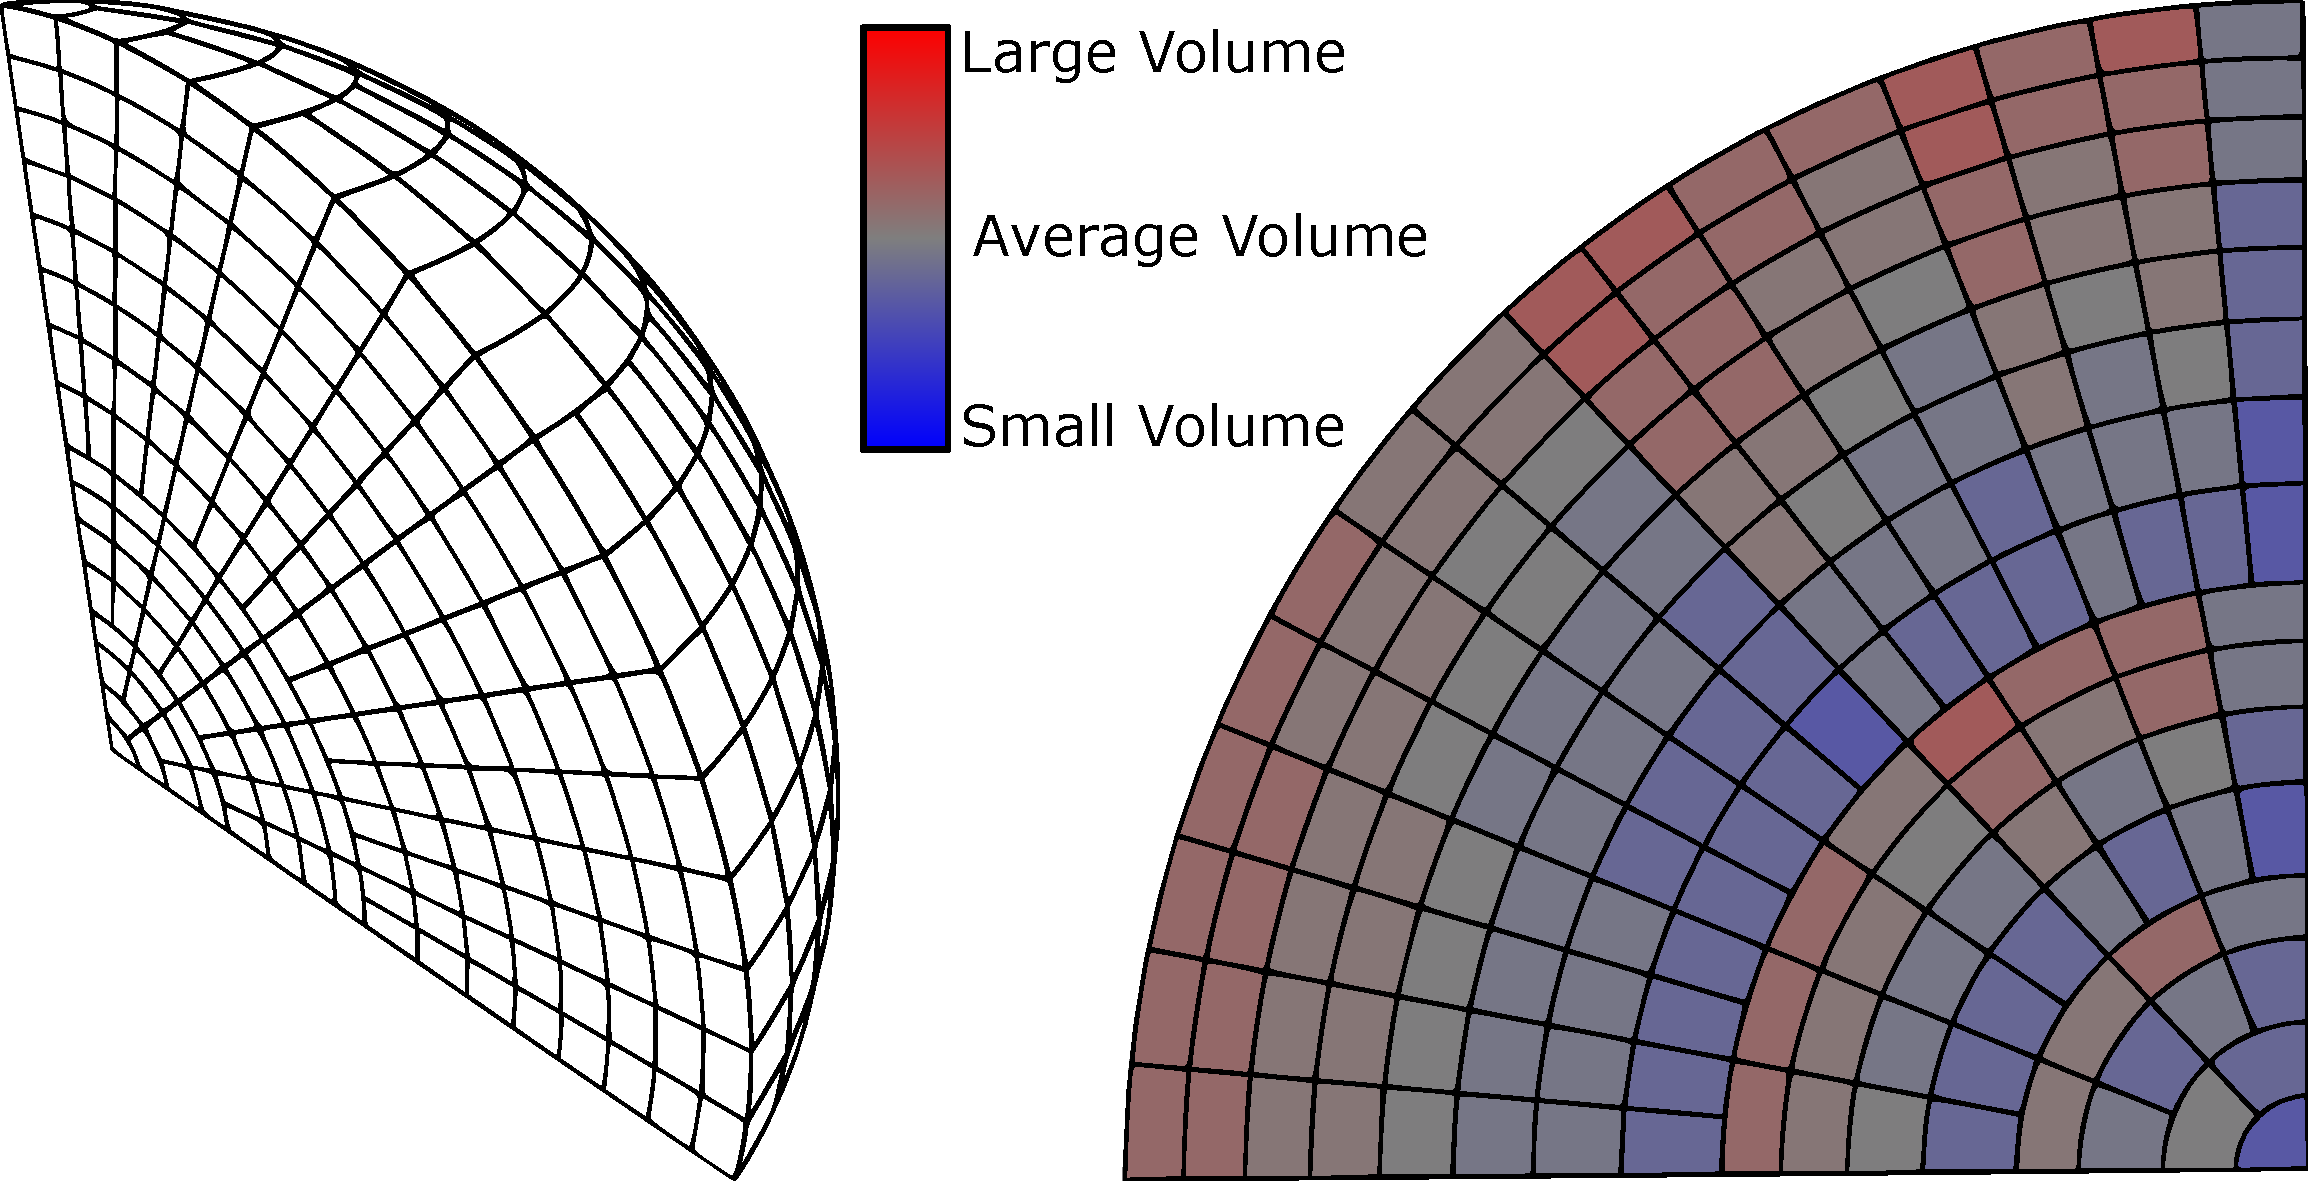
\includegraphics[width=0.85\textwidth]{Fig10.pdf}
	\caption{Results of the non-stationary scheme after four levels of subdivision using $\beta = \frac{1}{2}$.
		NG cells are still stretched and squashed in order to better preserve volume, however the effect is less pronounced}
	\label{fig:balanced}
\end{figure}


Figure~\ref{fig:perfect} shows the resulting grid from this method of calculating splitting surfaces.
In this grid, all NG cells at the same level of subdivision have exactly the same volume as one another.
This greatly improves the volume preservation, as only cells that extend to one of the poles (SG and LG cells) will have a different volume than the other cells in the grid.
This does not come without consequence though; cells are stretched and squashed in order to achieve this volume preservation, which may be an undesirable effect depending on the application.
To offset this reduction in cell compactness, it is possible to use splitting factors that are somewhere in between these ones ($c_{s}'$), which give ideal volume preservation, and the conventional SDOG ones ($c_{m}$), which give better compactness.
One simple way to calculate this would be as a convex combination of the two
%
\begin{equation}
c_{s} = \beta c_{s}' + \left( 1 - \beta \right)c_{m}, \quad \beta \in \left( 0,1 \right),
\label {eq:beta}
\end{equation}
%
however other methods could give better results.
We show a simple result in Figure~\ref{fig:balanced} using $\beta = \frac{1}{2}$.

\section{Results}
There are several potential methods for evaluating the volume preserving properties of a 3D DGGS.
When first proposed in \cite{yu2009sdog}, the ratio between cells of largest and smallest volume was used to evaluate volume preserving properties of SDOG.
This volume ratio is a useful measure for determining the worst-case difference in the volume of cells, however it does not give any information about the distribution of said volumes.
For example, a grid with all cells except one having equal volume, and a grid where every cell has a distinct volume, could end up having the same volume ratio.
To get a more complete understanding of volume preservation, we should also examine statistics that give a measure of distribution.
For this purpose, we use the coefficient of variation (CV), which is simply the ratio between the standard deviation and the mean.
We use the CV over the standard deviation as it a dimensionless quantity.


In modifying the subdivision for volume preservation, it is also important to evaluate the impact these changes have on other properties of the grid.
In Section \ref{sec:mapping} we discussed how the modified grids can be indexed using a mapping between them and conventional SDOG, however we should also measure the effect our changes have on the compactness of the resulting cells.
To measure this, we use the notion of sphericity, which quantifies how closely the shape of an object approximates a sphere~\cite{wadell1935volume}.
It is defined as the ratio between the surface area of a sphere with the same volume as the object and the surface area of the object itself.
Therefore, a perfect sphere will have a sphericity of one, and any other object will have sphericity strictly less than one.
Formally, given an object $\omega$ and a sphere $s$ such that $\operatorname{vol}(s) = \operatorname{vol}(\omega)$, the sphericity of $\omega$, $\Psi$, is given by $\frac{\operatorname{area}(s)}{\operatorname{area}(\omega)}$ , or equivalently 
%
\begin{equation}
\Psi = \frac{\pi^{\frac{1}{3}}\left( 6\operatorname{vol}(\omega) \right)^{\frac{2}{3}}}{\operatorname{area}(\omega)}.
\label{eq:sphericity}
\end{equation}
%
We use the mean and standard deviation (SD) of sphericity for all cells in the grid to evaluate compactness globally.


\begin{figure}[tbp]
	\centering
	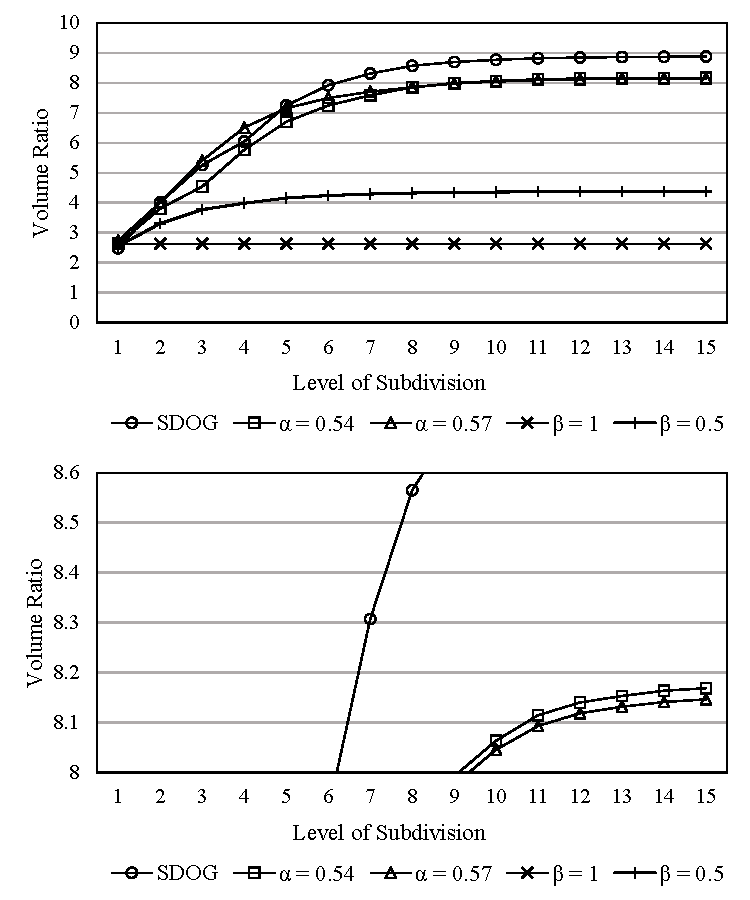
\includegraphics[width=0.75\textwidth]{Fig11.pdf}
	\caption{Volume ratio for the different grids at increasing levels of subdivision.
		Note that for the non-stationary method ($\beta = 1$) the volume ratio does not change with subdivision level}
	\label{fig:vr}
\end{figure}


\begin{figure}[tbp]
	\centering
	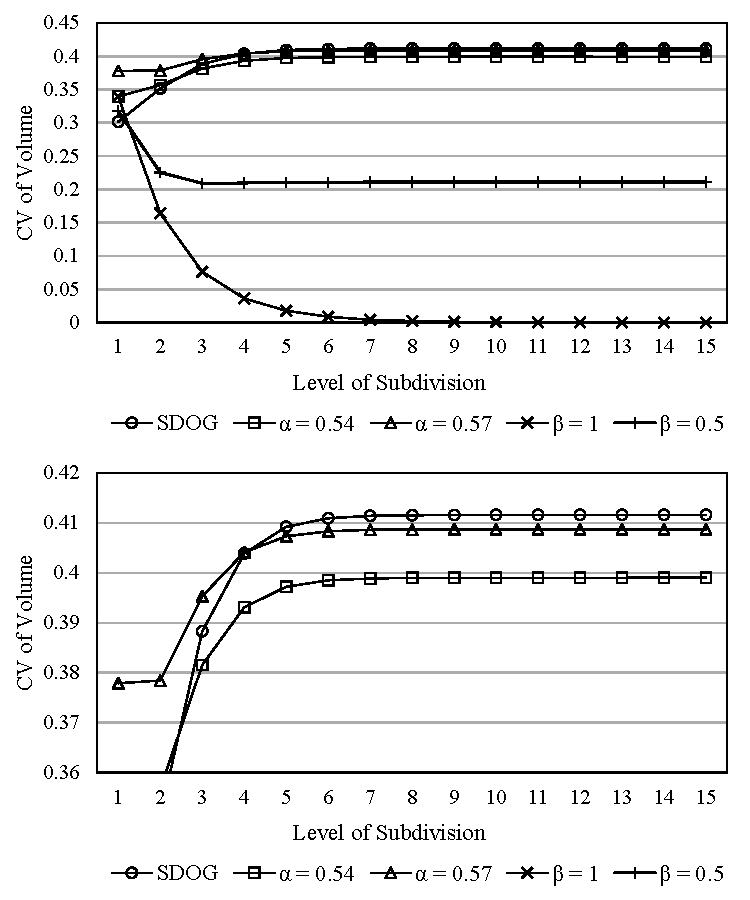
\includegraphics[width=0.75\textwidth]{Fig12.pdf}
	\caption{CV of volume for the different grids at increasing levels of subdivision}
	\label{fig:cv}
\end{figure}


\begin{figure}[tbp]
	\centering
	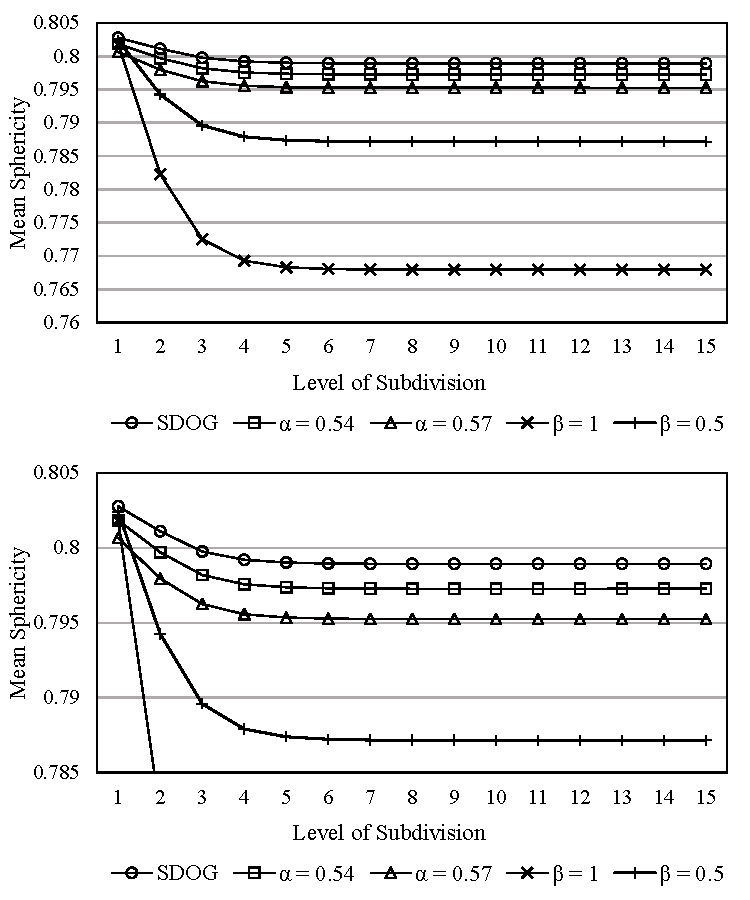
\includegraphics[width=0.75\textwidth]{Fig13.pdf}
	\caption{Mean sphericity for the different grids at increasing levels of subdivision}
	\label{fig:sph}
\end{figure}


\begin{figure}[tbp]
	\centering
	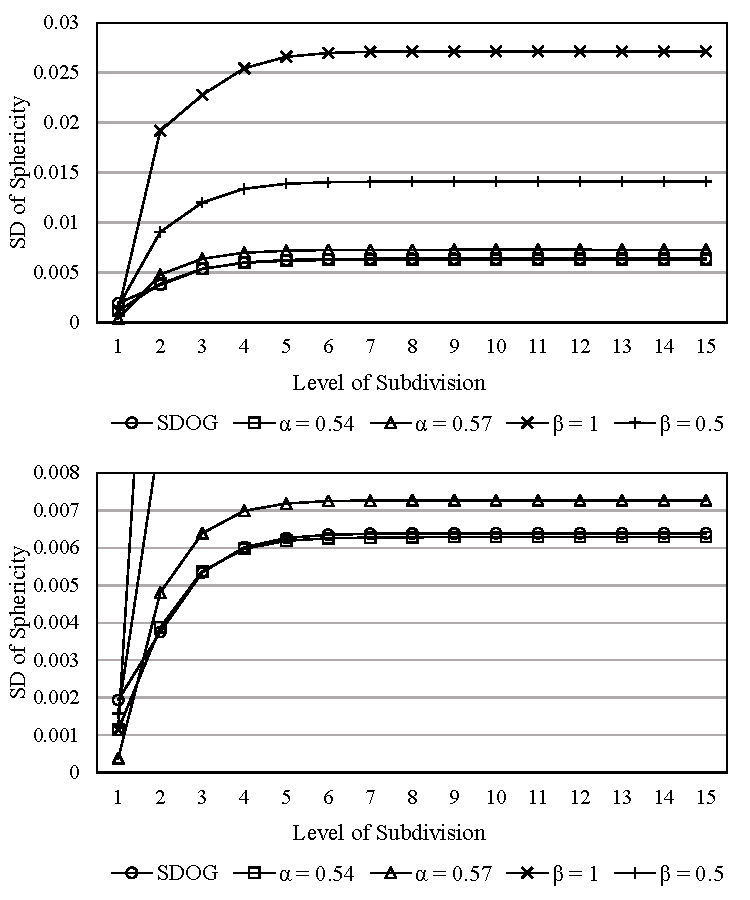
\includegraphics[width=0.75\textwidth]{Fig14.pdf}
	\caption{Standard deviation of sphericity for the different grids at increasing levels of subdivision}
	\label{fig:sd-sph}
\end{figure}


As a baseline, we have calculated the value of these measures at each subdivision level from one to fifteen for conventional SDOG.
We then repeated this for the four modifications discussed in this paper: the two stationary modifications with $\alpha_{\phi}^{SG} \approx 0.54$ and $\alpha_{\phi}^{SG} = 0.57$, the non-stationary modification (referred to as $\beta = 1$), and finally the blending of the non-stationary with conventional SDOG using $\beta = \frac{1}{2}$.
The results for each grid are displayed in Figures~\ref{fig:vr}, \ref{fig:cv}, \ref{fig:sph}, and \ref{fig:sd-sph} showing the volume ratio, CV of volume, mean sphericity, and SD of sphericity respectively.
Table~\ref{tab:results} summarizes these charts with the convergence value of each property for the five different grids.
We also give convergence values for the maximum and minimum sphericity---and their difference---for each grid in Table~\ref{tab:results-sph}.
It is important to note that for volume ratio and CV of volume lower values are better, but for mean sphericity a higher value is better.


\begin{table}[]
	\centering
	\caption{Convergence value of each measure for the five discussed grids}
	\begin{tabular}{|c|c|c|c|c|c|}
		\hline
		& SDOG & $\alpha_{\phi}^{SG} \approx 0.54$ & $\alpha_{\phi}^{SG} = 0.57$ & $\beta = 1$ & $\beta = 0.5$ \\ \hline
		Volume Ratio     & 8.88   & 8.17   & 8.15   & 2.63      & 4.37   \\ \hline
		CV of Volume     & 0.412  & 0.399  & 0.409  & 6.44E-19  & 0.211  \\ \hline
		Mean Sphericity  & 0.799  & 0.797  & 0.795  & 0.767     & 0.787  \\ \hline
		SD of Sphericity & 0.00639& 0.00629& 0.00727& 0.0271    & 0.0141 \\ \hline
	\end{tabular}
	\label{tab:results}
\end{table}


\begin{table}[]
	\centering
	\caption{Convergence value of max and min sphericity for the five discussed grids}
	\begin{tabular}{|c|c|c|c|c|c|}
		\hline
		& SDOG & $\alpha_{\phi}^{SG} \approx 0.54$ & $\alpha_{\phi}^{SG} = 0.57$ & $\beta = 1$ & $\beta = 0.5$ \\ \hline
		Max sphericity & 0.806  & 0.806  & 0.806  & 0.806 & 0.806  \\ \hline
		Min sphericity & 0.754  & 0.763  & 0.766  & 0.672 & 0.728  \\ \hline
		Difference     & 0.0520 & 0.0428 & 0.0404 & 0.134 & 0.0780 \\ \hline
	\end{tabular}
	\label{tab:results-sph}
\end{table}


The stationary scheme with $\alpha_{\phi}^{SG} \approx 0.54$ has a better volume ratio than conventional SDOG for all levels of subdivision except the first, and a lower CV of volume for all levels of subdivision after the second.
Comparing this to the one with $\alpha_{\phi}^{SG} = 0.57$, both the volume ratio and CV of volume do not improve as compared to conventional SDOG until the fifth level of subdivision.
Both of these methods also reduce the mean sphericity of cells at all levels of subdivision, with $\alpha_{\phi}^{SG} = 0.57$ having more than twice the absolute reduction of $\alpha_{\phi}^{SG} \approx 0.54$.
The variation in sphericity is similar between all three of these grids.
Using $\alpha_{\phi}^{SG} = 0.57$ does give a slightly better volume ratio than $\alpha_{\phi}^{SG} \approx 0.54$ as the level of subdivision gets large, however this difference is quite small and likely not worth the lower cell compactness and higher variation in volume.


The non-stationary scheme gives a much larger improvement to both the volume ratio and the CV of volume.
This is to be expected, as all NG cells in this scheme have exactly equal volume.
As the level of subdivision gets large, the CV of volume quickly approaches zero since the number of NG cells is much larger than the number of LG and SG cells in the grid.
The cost of this improved volume preservation is a much larger reduction in the sphericity of cells and an increase in the variation of sphericity, which is to be expected.
The blending scheme has results in between that of conventional SDOG and the non-stationary scheme, which was also expected.
The CV of volume, mean sphericity, and SD of sphericity are all near the respective halfway points, whereas the volume ratio still ends up being a significant improvement over conventional SDOG.

\section{Summary}
\chapter{Extending Geodesic DGGSs to Create 3D Prismatoid Grids} \label{chap:extension}

\section{Prismatoid Grid Generation and Refinement}
Using the input DGGS as an input specification, our goal is to define the key elements of the corresponding 3D DGGS logically and consistently.
In this section, we discuss the approach for generating the initial discretization and define two refinement methods.


\subsection{Initial 3D Discretization} \label{sec:grid:discretization}
The initial 3D discretization is generated from the input polyhedron by extruding each face to cover the desired radial extent of the grid.
Faces are extruded outward to the desired maximum altitude, $R_\mathrm{max}$, and inwards to the desired minimum altitude, $R_\mathrm{min}$ (Figure~\ref{fig:abstract} top right).
These values become the maximum and minimum supported radii of the 3D DGGS, respectively.
If the minimum radius is zero, these base cells are pyramids; otherwise, they are frusta.
In both cases, the cells belong to a parent class of polyhedra known as prismatoids.
With this discretization, each cell represents the full radial domain of the grid; subsequent refinements will address this issue.


\subsection{Regular Prismatoid Refinement} \label{sec:grid:regular}
With an initial 3D discretization for the space of the grid system, we now need a method for refining cells to create more fine discretizations.
We also want to ensure that the 3D DGGS will make use of the same refinement scheme used by the input DGGS, referred to as the surface refinement.
For simplicity, we initially assume the surface refinement factor is 1:4; a generalization to other refinement factors is given in Section~\ref{sec:grid:factors}.


\begin{figure}[h]
	\centering
	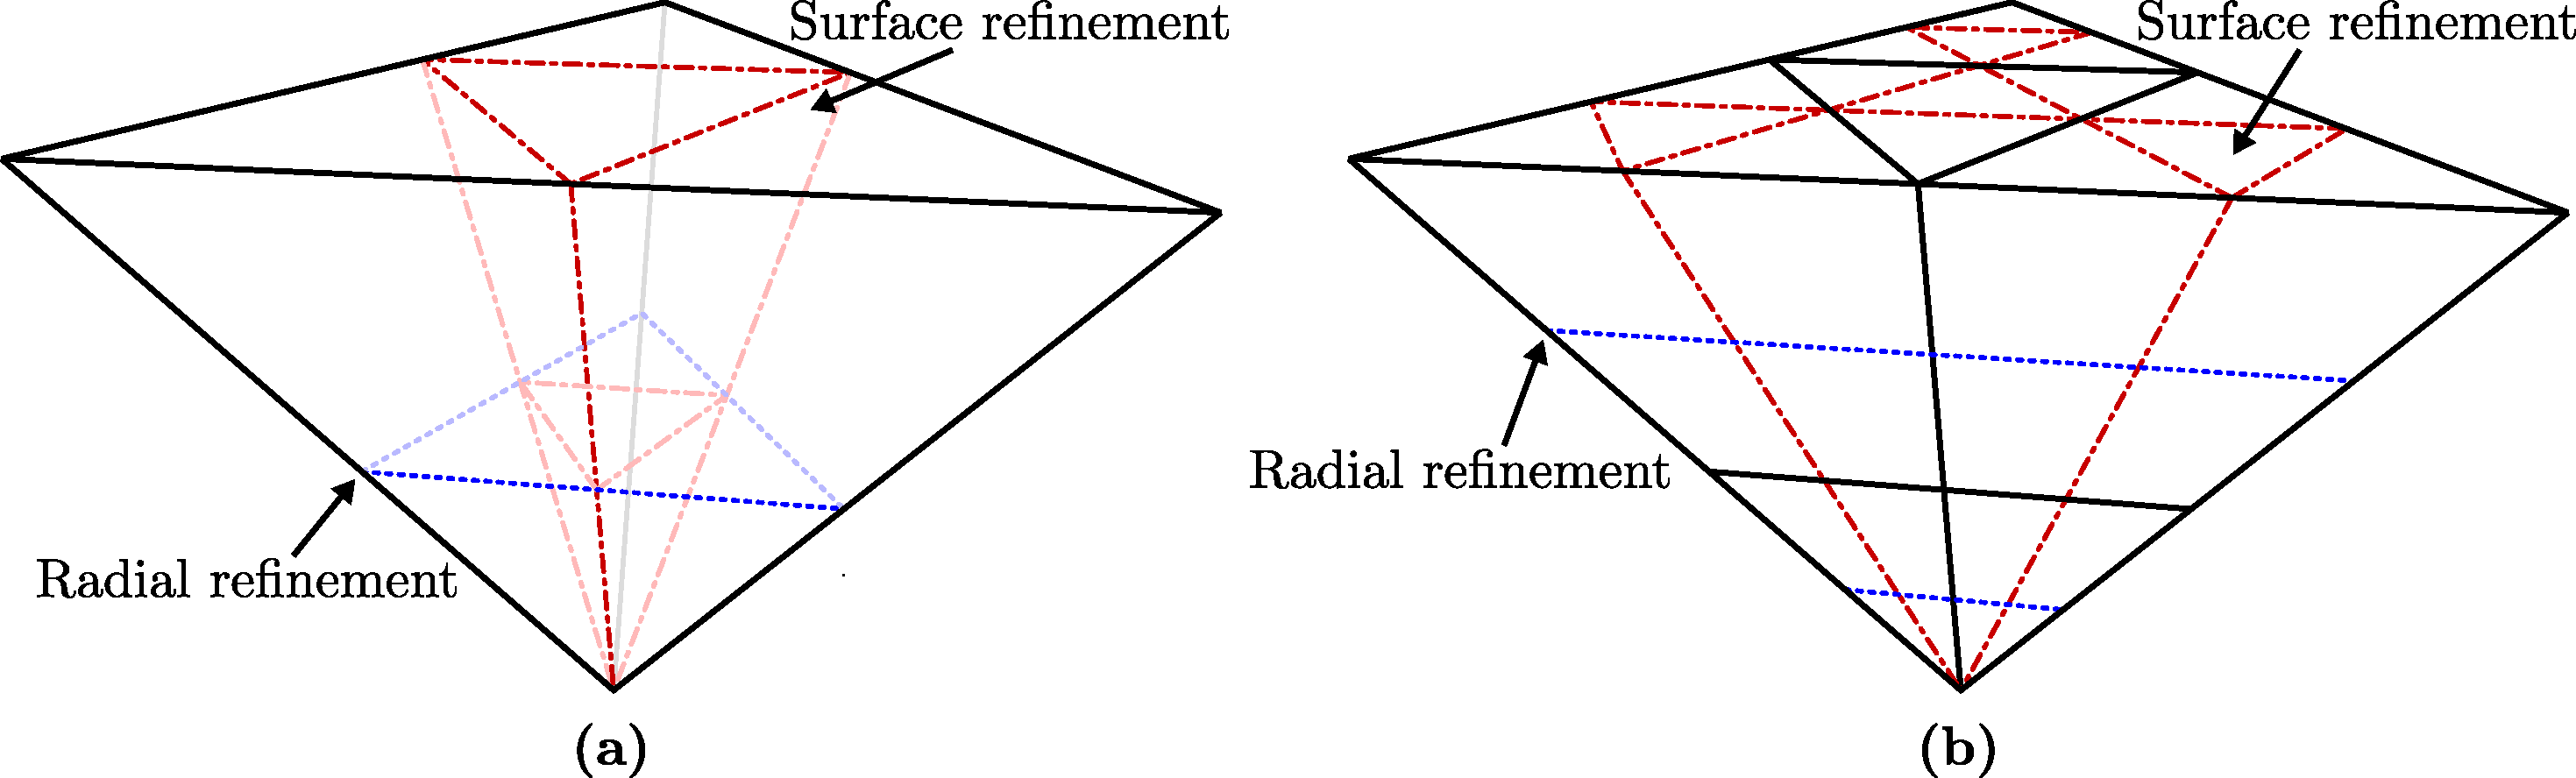
\includegraphics[width=\columnwidth]{basic-refinement.pdf}
	\caption{Regular prismatoid refinement as applied to a single pyramid cell \textbf{(a)} once and \textbf{(b)} twice}
	\label{fig:regular}
\end{figure}


The regular method for refining prismatoid cells is shown in Figure~\ref{fig:regular}.
The bases of the cells are refined using the surface refinement and the resulting edges extruded to meet.
At the same time, a radial split is placed at the midpoint between the two bases.
This refinement results in an inner and outer layer of cells, each containing the same number of cells as one another.
The outer layer is always composed of frustum cells, whereas the inner layer has the same shape as the cells that were being refined.
This refinement can then be repeated, treating each of the new layers the same as the initial discretization.
Defining the refinement in terms of layers of cells as opposed to individual cells allows non-congruent surface refinements to be accommodated inherently.


\subsection{Semiregular Prismatoid Refinement} \label{sec:grid:degen}
While the regular prismatoid refinement proposed above is simple, it has a key drawback if the ratio between $R_\mathrm{max}$ and $R_\mathrm{min}$ is large.
In this situation, layers that are near the minimum radius end up being much smaller than those near the maximum.
A different refinement method is needed to generate more uniformly sized cells.
To do this, we classify the layers of the grid as either central or normal.
We use $r_\mathrm{min}$ and $r_\mathrm{max}$ to refer to the minimum and maximum radius of a layer, respectively.
Central layers are those that border the innermost portion of the grid ($r_\mathrm{min} = R_\mathrm{min}$) and all other layers are considered normal.
By definition, at any resolution of the 3D DGGS, there is only one central layer.
Furthermore, the initial discretization is entirely composed of this central layer.
We continue our assumption of a 1:4 surface refinement factor from before.


\begin{figure}[h]
	\centering
	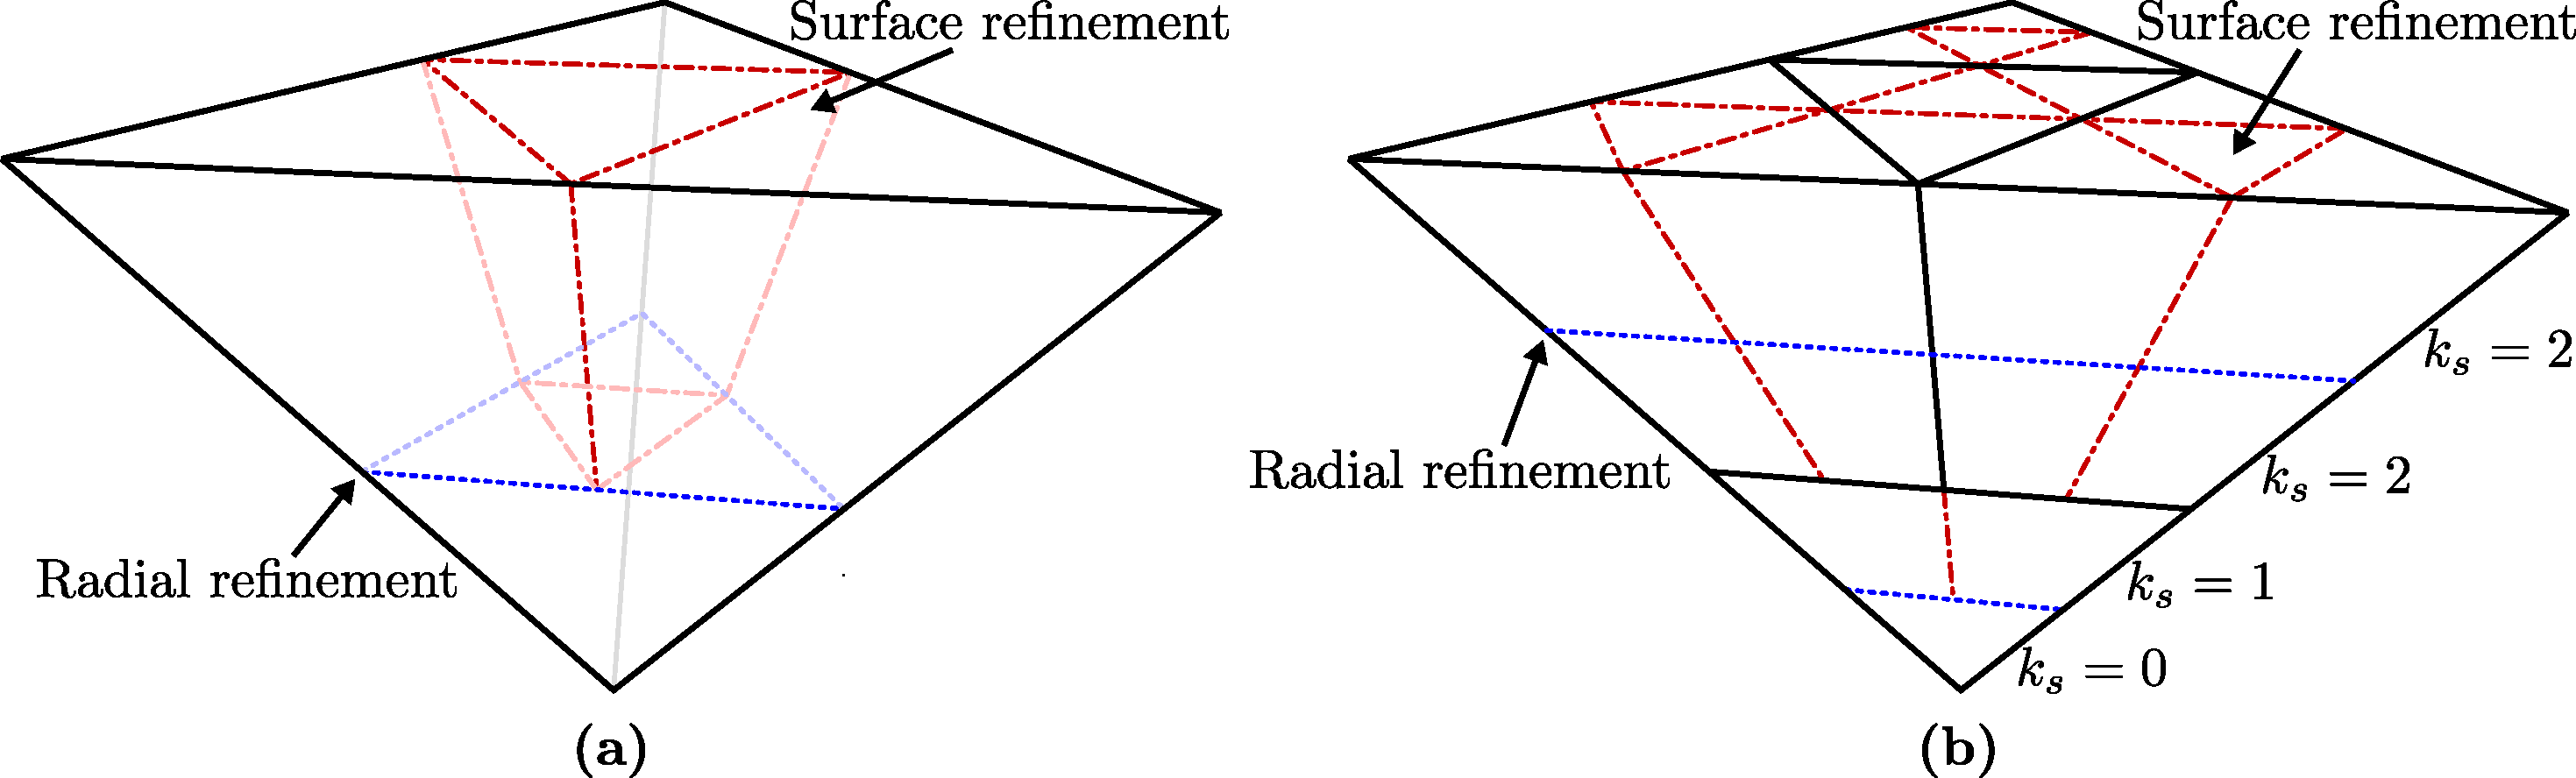
\includegraphics[width=\columnwidth]{degen-refinement.pdf}
	\caption{Semiregular prismatoid refinement as applied to a single pyramid cell \textbf{(a)} once and \textbf{(b)} twice.
		In \textbf{(b)}, the number of times the surface refinement has been applied ($k_s$) is shown for each layer; see how the radial refinements of central layers separate regions of the grid with different values of $k_s$}
	\label{fig:semiregular}
\end{figure}


In this refinement scheme, refinement of central layers is different from the above regular method.
We assert that $R_\mathrm{min}$ be treated as equal to zero, and therefore central layers are composed of pyramid cells.
If the actual value of $R_\mathrm{min}$ is not zero, then any resulting layers below this radius can be discarded or ignored.
Just as before, the bases of the pyramid cells are refined using the surface scheme, and a radial split is made in the middle of the layer.
However, the new edges do not extend fully toward the apex of the pyramid but instead are stopped at the radial split (Figure \ref{fig:semiregular}).
This refinement results in two new layers: an inner central layer, which is similar to the initial central layer, and an outer normal layer.
As demonstrated in Figure~\ref{fig:semiregular}b, the resolution---or refinement level---a layer appears in at the 3D grid does not necessarily correspond to how many times the surface refinement scheme has been applied to it.
We define the number of times the surface refinement has been applied to a given layer as the surface resolution, given by $k_s$.
Thus, if we say the initial discretization has $k_s = 0$, after one level of refinement the inner central layer also has $k_s = 0$, whereas the normal layer has $k_s = 1$.
This surface resolution is needed for grid encoding/decoding and various indexing queries, but as will be seen later can be computed and does not need to be explicitly stored.


\begin{figure}[h]
	\centering
	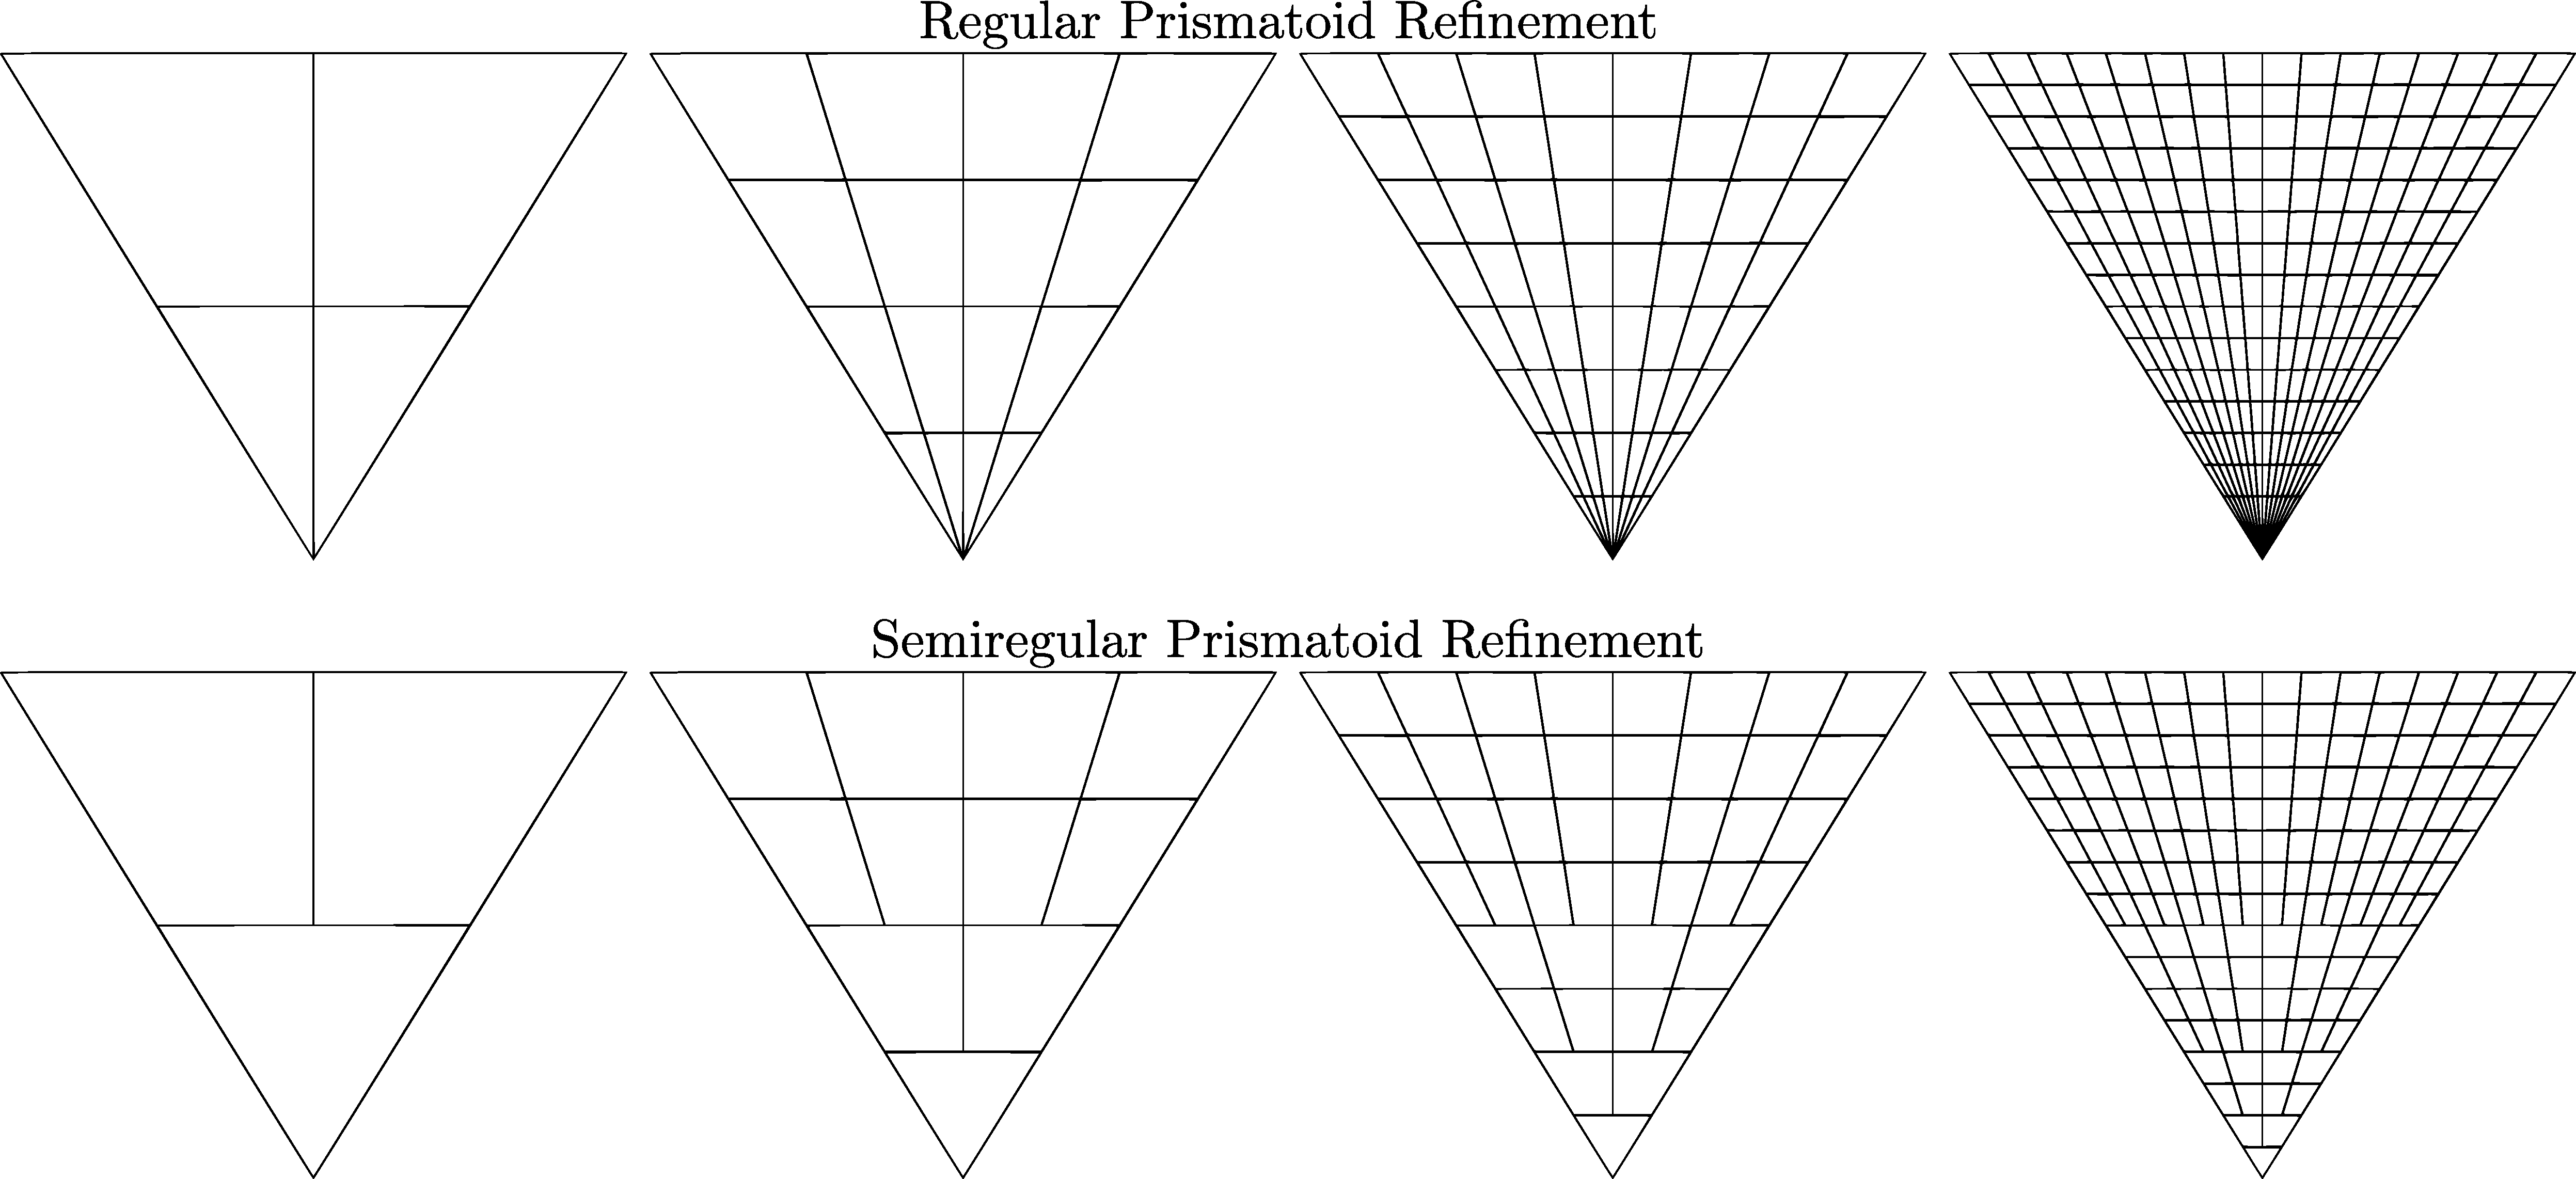
\includegraphics[width=\textwidth]{comparison.pdf}
	\caption{Three levels of successive applications of regular (top) and semiregular (bottom) prismatoid refinement.
		Only the side of a single pyramid starting cell is shown to highlight the behaviour of the two schemes at different radii.
		Note how cells degenerate towards the centre with regular refinement, whereas this issue is not present in the semiregular scheme}
	\label{fig:multipleSL}
\end{figure}


Normal layers in this scheme are simply refined using regular prismatoid refinement.
This results in two normal layers, both of which have $k_s$ equal to one greater than that of the starting layer.
Figure~\ref{fig:multipleSL} compares three successive applications of regular and semiregular prismatoid refinement to a single pyramid cell.

\section{Refinement Extensions}
\subsection{Other Surface Refinement Factors} \label{sec:grid:factors}
While it is possible to use the above refinement methods for surface refinement factors other than 1:4, doing so results in a potentially significant issue that should be addressed.
To address this challenge, we introduce the idea of a one-dimensional (1D) refinement factor.
We can find the 1D refinement factor by taking the square root of the surface (2D) one.
For example, the 1D refinement factor of a 1:4 surface refinement scheme (Figures~\ref{fig:regular} and \ref{fig:semiregular}) is 1:2.
While the surface refinement scheme need not be uniform across the two dimensions, the 1D refinement factor gives an idea of the \textit{average} refinement that is expected along each dimension.


To create uniform cells, it is clear that the refinement factor along the radial dimension for regular prismatoid refinement should be equal to the 1D refinement factor.
If this is not the case, then the width of cells relative to their depth is not constant between refinement levels, since one dimension is refined more quickly.
For a surface refinement factor of 1:4, the single radial split used matches this exactly (one split creates two new layers).
For other surface refinement factors, the 1D and radial refinement factors are not necessarily equal, and cell shape will degenerate---becoming either increasingly narrow or wide---as refinement continues.


To address this issue, we modify the number of radial splits performed such that the number of layers produced is equal to the 1D refinement factor.
For surface refinement factors that are perfect squares (e.g.
1:4, 1:9) this is trivial, as the 1D refinement factor is an integer; the corresponding radial refinement factor is achieved by creating a number of layers equal to the 1D factor.
For other surface refinement factors, though, this becomes more difficult.
The 1D refinement factor is no longer an integer, and since we can only perform a whole number of radial splits, the 1D and radial refinement factors cannot be exactly equal.
To address this issue, we propose performing a different number of radial splits at different levels of refinement to make the average radial refinement factor equal to the 1D one.


There are a few different methods that can be used to determine the number of radial splits to perform at a given refinement level.
The most simple method is to simply alternate between producing one layer (i.e.
no splits) and producing a number of layers equal to the surface refinement factor.
When the surface refinement factor is not a prime number, a better method is to alternate between the two members of a factor pair, such as two and three for a 1:6 surface factor.
In general, the product of the number of layers at each level of refinement should be equal to (or as close as possible to) the 1D refinement factor to the power of the number of refinement levels.
Formally,

\begin{equation*}
\prod_{i = 1}^{k} \ell_{i} = f^{k},
\end{equation*}
%
where $\ell_{i}$ is the number of layers produced at refinement level $i$, $k$ is the level of refinement, and $f$ is the 1D refinement factor.
This equation can be used iteratively to find the best number of layers for successive levels of refinement for prime surface refinement factors.
Table~\ref{tab:layers} lists our proposed layering sequences for surface refinement factors from 1:2 up to 1:9.


\begin{table}[h]
	\centering
	\begin{tabular}{@{}cl@{}}
		\toprule
		Surface Refinement Factor & Layering Sequence       \\ \midrule
		1:2                  & \textbf{2,1,2,1}             \\ 
		1:3                  & \textbf{3,1,3,1}             \\ 
		1:4                  & \textbf{2,2,2,2}             \\ 
		1:5                  & 2,3,2,2,2,3,2,2,2,3,2,2,3... \\ 
		1:6                  & \textbf{3,2,3,2}             \\ 
		1:7                  & 3,2,3,3,2,3,3,2,3,3,3,2,3... \\ 
		1:8                  & \textbf{4,2,4,2}             \\
		1:9                  & \textbf{3,3,3,3}             \\ \bottomrule
	\end{tabular}
	\caption{Our proposed layering sequences for different surface refinement factors.
		Each number in the sequence is how many layers \textit{normal} layers should split into at the corresponding level of refinement.
		Bold indicates that the sequence repeats indefinitely.
		For semiregular prismatoid refinement---since the initial discretization has no normal layers---these sequences are used starting with the \textit{second} level of refinement}
	\label{tab:layers}
\end{table}


\begin{figure}[h]
	\centering
	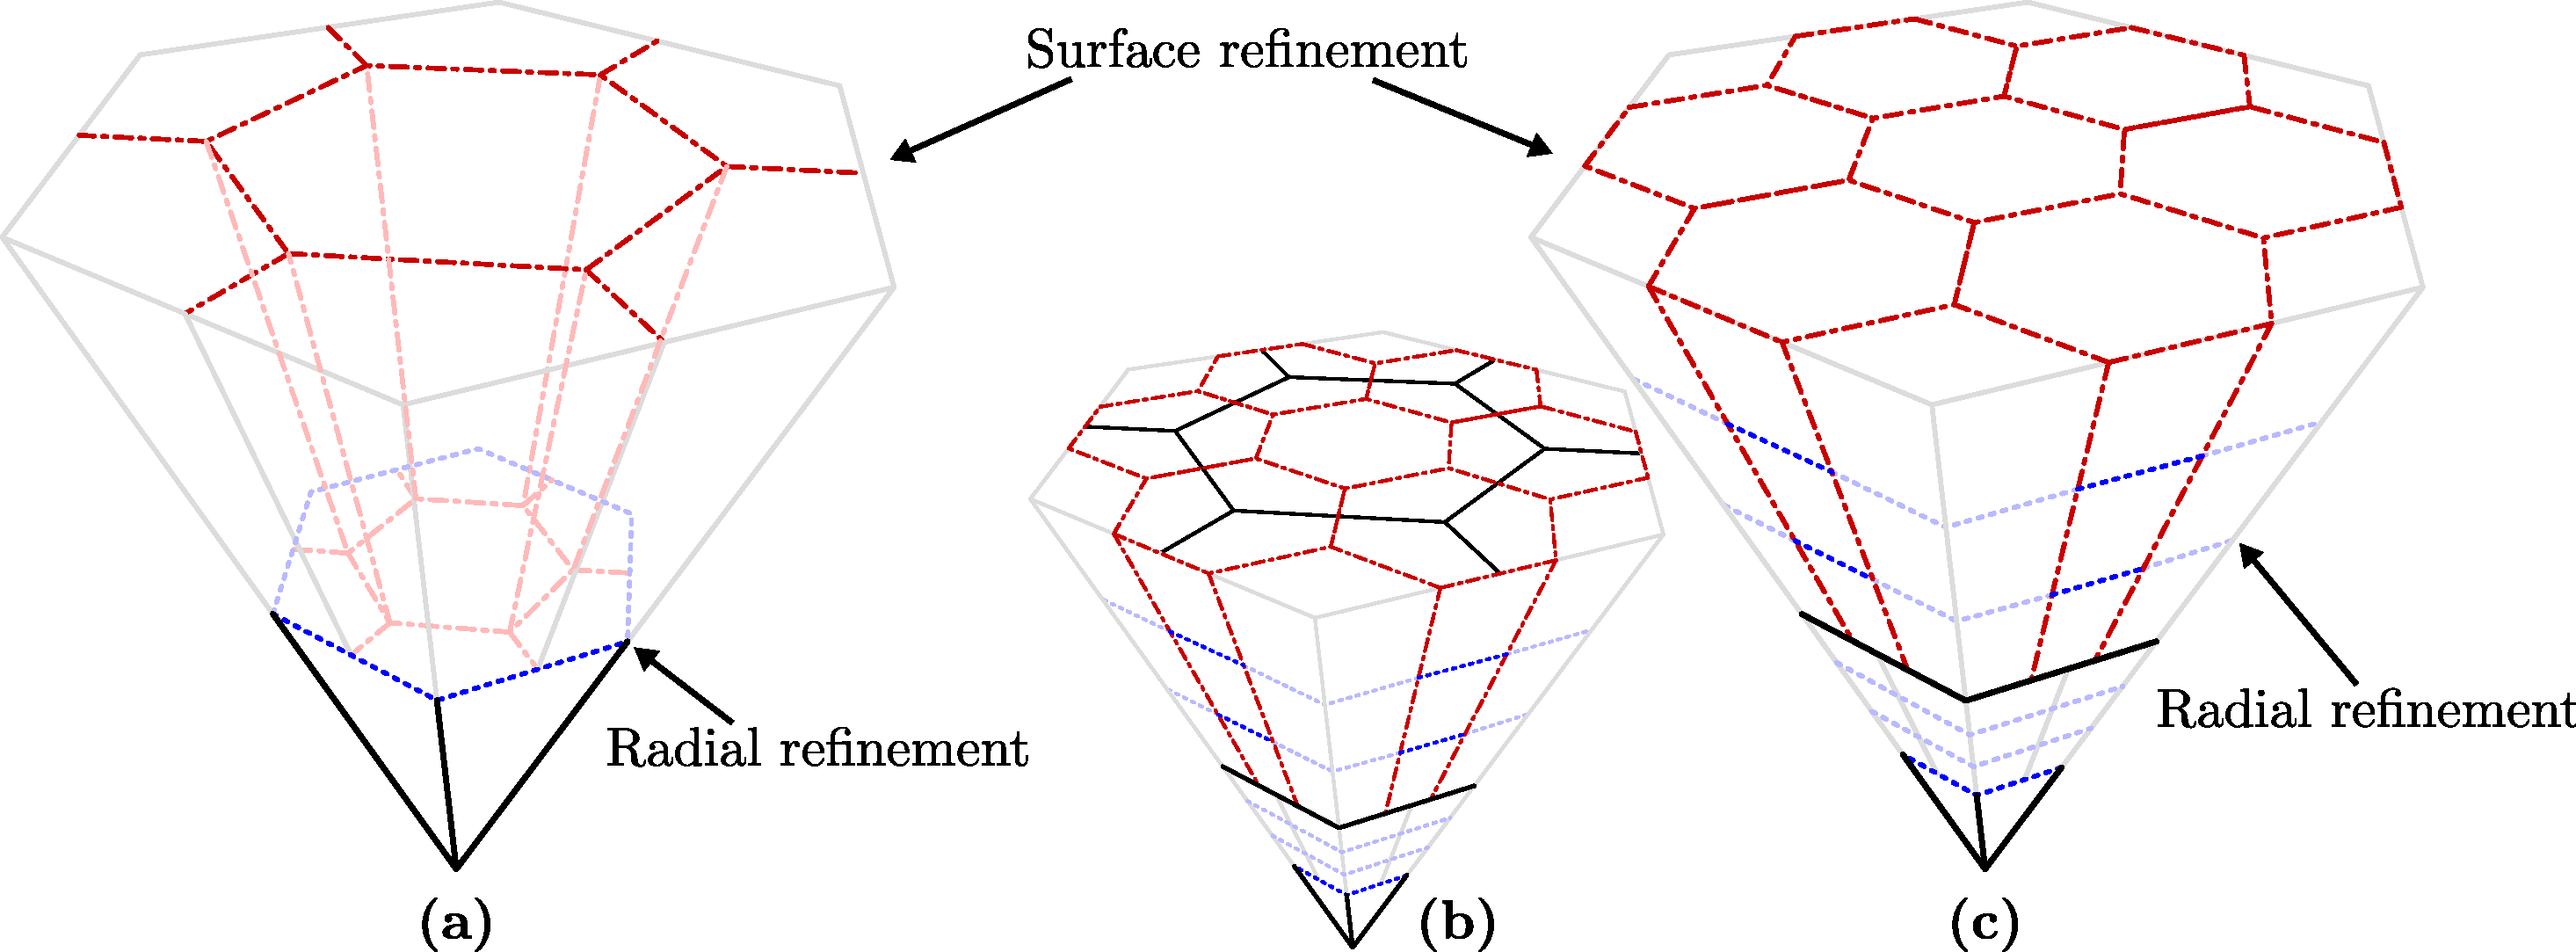
\includegraphics[width=\textwidth]{hexagons.pdf}
	\caption{Semiregular prismatoid refinement applied to a hexagonal base cell using a 1:3 surface refinement scheme \textbf{(a)} once and \textbf{(c)} twice; \textbf{(b)} is the same image as \textbf{(c)}, but with the surface cells of the previous refinement level shown for reference.
		Note that in the second level of refinement, normal layers have two radial refinements as opposed to one}
	\label{fig:hexagons}
\end{figure}


An example of semiregular prismatoid refinement with 1:3 hexagonal surface refinement is shown in Figure~\ref{fig:hexagons}.
The first level of refinement is identical to the cases for a 1:4 surface refinement factor since no normal layers have been refined.
In the second level, however, two radial splits are performed in the normal layers as opposed to one.
In the next level of refinement, which is not shown, normal layers would not have any radial refinements per the proposed sequence in Table~\ref{tab:layers}.


\subsection{Cell Aspect Ratio} \label{sec:grid:ar}
The surface and radial dimensions of Earth are inherently very different, and because of this, it is often desirable for these two dimensions to be at different resolutions in a 3D geospatial grid.
For our 3D DGGSs, achieving this entails changing the width of cells in the grid (surface resolution) relative to their depth (radial resolution).
We refer to the ratio between a cell's width and depth the \textit{aspect ratio} of the cell.
While the refinement methods described thus far do a good job of producing cells with a similar aspect ratio---both between cells in the same and different resolutions---there is no direct mechanism for controlling what this aspect ratio will be.
To address this issue, we introduce two modifications that can be made to prismatoid refinement to decrease and increase the aspect ratio.


In order to decrease the aspect ratio of cells in the grid, the number of times the surface refinement is applied relative to the number of radial splits should be increased.
Since further applications of the prismatoid refinement will maintain the expected cell aspect ratio (a result of the surface and expected radial refinement factors being equal), this only needs to be done the first time a layer would have the bases of its cells refined with the surface scheme.
Thus, for semiregular prismatoid refinement, this is done while refining the outer normal layer that results from refining central layers.
In the case where only regular prismatoid refinement is used, this is then only done during the first level of refinement.


Likewise, to increase the aspect ratio of cells, we need to decrease the number of times the surface refinement scheme is applied relative to the number of radial splits.
This is done by first \textit{not} applying the surface refinement to a layer the first time it would usually be done, and if needed applying additional radial splits at the same time.
These modifications would be done at the same time as the method for decreasing the aspect ratio for the same reasons.


Therefore, given some target cell aspect ratio $a$, we must determine which of the above methods to use.
To do this, we must first quantify the width and depth of a cell.
More specifically, we need to define the average width and depth of cells in a layer, since refinement is performed by layer and not by cell.
Depth comes trivially from the radial extent of the layer ($r_\mathrm{max} - r_\mathrm{min}$).
There are many potential ways to measure the width of a cell; for our purposes, we chose to use the square root of its area.
This choice ensures the framework will produce consistent results for input polyhedra with the same number of faces, irrespective of the shape(s) of said faces.


For the region of outer normal layer(s) generated by refining central layers, we can say the average depth of cells is the total depth of the region divided by the number of layers in the region (assuming no applications of the surface refinement scheme).
Let $\upsilon$ be the percentage of $r_\mathrm{max}$ occupied by this region and $x$ be the number of extra radial splits, then we have

\begin{equation*}
\frac{\upsilon r_\mathrm{max}}{x+1}.
\end{equation*}
%
Likewise, the average cell width in this region is the surface area of the sphere divided by the number of cells (assuming no extra radial splits).
Let $n$ be the number of faces on the input polyhedron and $w$ be the number of times the surface refinement is applied, then the number of cells is $n f^{2w}$ and the average cell width is

\begin{equation*}
\sqrt{ \frac{ 4 \pi r_\mathrm{max}^2 }{ n f^{2 w} } } = \frac{2 r_\mathrm{max}}{f^w} \sqrt\frac{\pi}{n}.
\end{equation*}
%
We can now equate these using the desired aspect ratio to solve for $x$ and $w$, giving

\begin{equation*}
a \frac{\upsilon}{x+1} = \frac{2}{f^w} \sqrt\frac{\pi}{n}.
\end{equation*}
%
As to not violate our prior assumptions, when solving for one variable the other is set to zero; this ensures only one of the two strategies for modifying the aspect ratio is employed.
Setting $w = 0$ we get

\begin{equation}
x = \frac{a \upsilon}{2} \sqrt{\frac{n}{\pi}} - 1,
\label{eq:extraSplits}
\end{equation}
%
and setting $x = 0$ we get

\begin{equation}
w = \log_{f} \left( \frac{2}{a \upsilon} \sqrt{ \frac{\pi}{n}} \right).
\label{eq:num2D}
\end{equation}


\begin{figure*}[h]
	\centering
	\begin{subfigure}[]{0.25\textwidth}
		\centering
		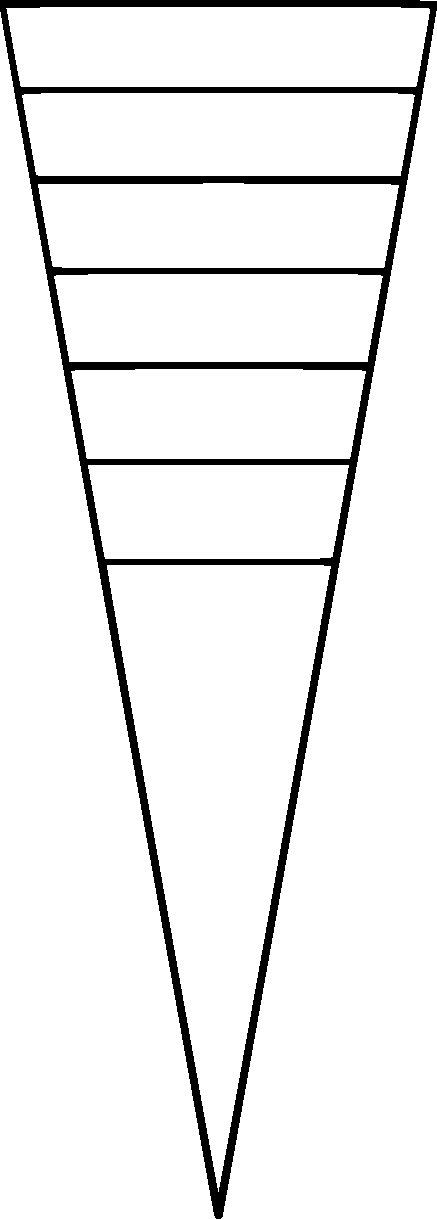
\includegraphics[width=0.5\columnwidth]{5-ers.pdf}
		\caption{}
		\label{fig:ers1}
	\end{subfigure}%
	%
	\begin{subfigure}[]{0.25\textwidth}
		\centering
		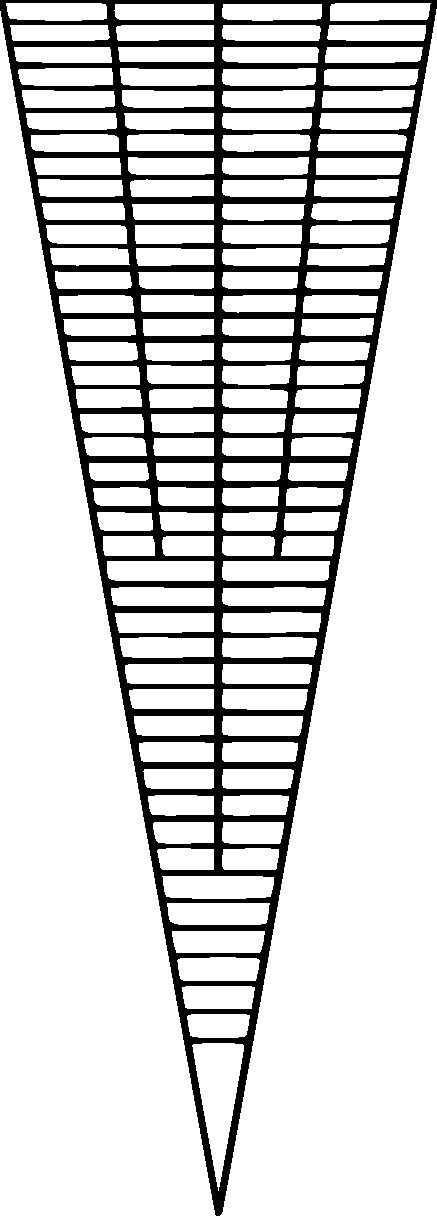
\includegraphics[width=0.5\columnwidth]{5-ers3.pdf}
		\caption{}
		\label{fig:ers3}
	\end{subfigure}%
	%
	\begin{subfigure}[]{0.25\textwidth}
		\centering
		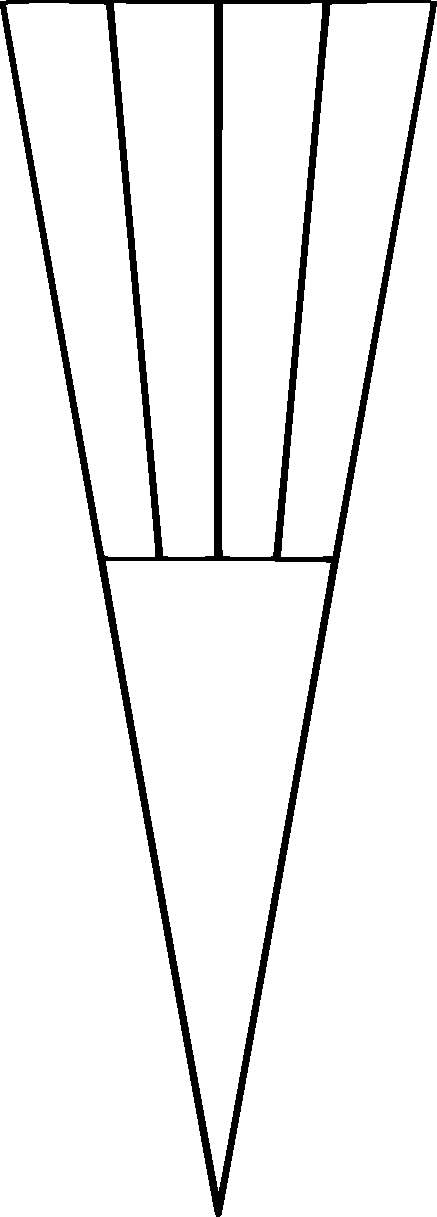
\includegraphics[width=0.5\columnwidth]{2-ess.pdf}
		\caption{}
		\label{fig:ess1}
	\end{subfigure}%
	%
	\begin{subfigure}[]{0.25\textwidth}
		\centering
		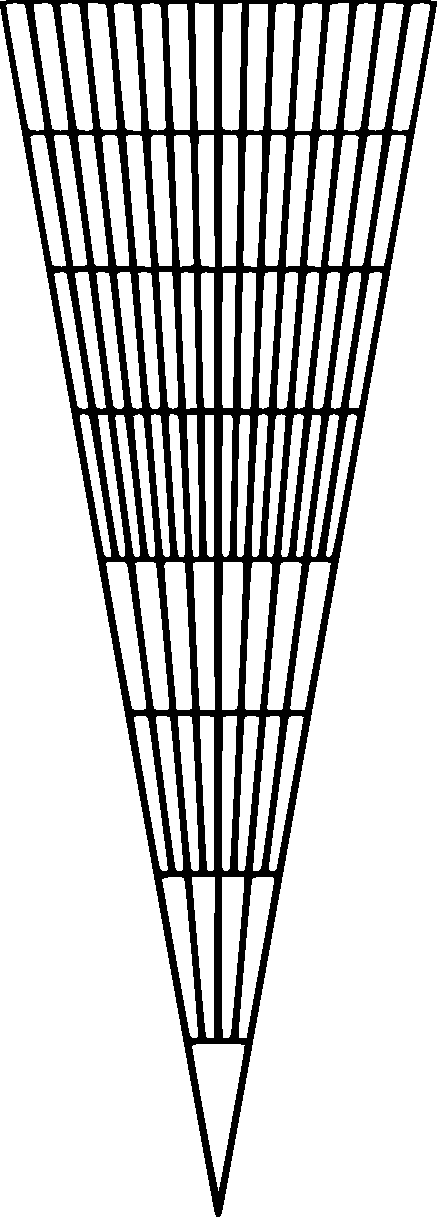
\includegraphics[width=0.5\columnwidth]{2-ess3.pdf}
		\caption{}
		\label{fig:ess3}
	\end{subfigure}
	
	\caption{A demonstration of how refinement can be modified to affect the aspect ratio of cells.
		All figures show a starting pyramid cell from a grid with 200 cells in its initial discretization.
		Central layer with five extra radial splits ($a = 3$ to get $x = 5$) at \textbf{(a)} one level of refinement and \textbf{(b)} three levels.
		Central layer with two applications of the surface refinement scheme ($a = 1/8$ to get $w = 2$) at \textbf{(c)} one level of refinement and \textbf{(d)} three levels}
	\label{fig:extraDPS}
\end{figure*}


The actual values of $x$ and $w$ selected for use is determined by which one is negative.
If $x$ is negative, it is set to zero, and the value of $w$ is used---vice versa for if $w$ is negative.
Since $x$ or $w$ may not be integers, we simply round them to the nearest whole number to get the actual value to be used during refinement.
The results of refinement with different target aspect ratios are demonstrated in Figure~\ref{fig:extraDPS}.

\section{Results}
\section{Summary}
\chapter{Mapping Techniques for SDOG and Prismatoid Grids} \label{chap:mapping}

\section{Radial Mappings}
\section{Latitude Mappings for SDOG}

%\section{Mapping Modified SDOG Grids} \label{sec:mapping}
By modifying the splitting surfaces used for subdivision, any SDOG indexing operations that depend on the location of cells in the grid will no longer function properly.
Examples of these operations include point to cell queries, which give the cell that contains a given point, and index inversion, which calculates the location and geometry of a cell from its index.
The obvious solution is to simply redefine these operations on the new geometry, however, this is not necessarily practical as it would have to be done individually for each modified grid.
Additionally, the more complex geometry of the modified grids may make these algorithms more difficult to design and/or more computationally expensive to perform as compared to the ones for conventional SDOG.
A better solution is to find a mapping (and corresponding inverse mapping) between a conventional SDOG grid and the grid resulting from the modified subdivision scheme.
Given this mapping, all indexing operations can be done using the standard algorithms, with inputs and outputs converted between the conventional SDOG grid and the modified one accordingly.


For the stationary subdivision schemes this mapping is straightforward.
Since only the latitudinal splitting surface of SG cells is modified, latitudes in the range $[0, \pm\frac{\pi}{4})$ should be mapped to the range $[0, \pm\alpha_{\phi}^{SG} \frac{\pi}{2})$ and likewise the range $[\pm\frac{\pi}{4}, \pm\frac{\pi}{2}]$ to the range $[\pm\alpha_{\phi}^{SG} \frac{\pi}{2}, \pm\frac{\pi}{2}]$.
This can be done with a simple linear map, and the inverse follows trivially.


For the non-stationary schemes this mapping is more complicated.
We wish to define a function $M \colon (\phi, r) \rightarrow (\phi, r)$ that converts a latitude and radius in a conventional SDOG grid to the corresponding latitude and radius in the modified grid (longitude does not need to be mapped, as it is not changed between the two grids).
The two coordinates act independently of each other, so we can split this function into its two components, $M_{\phi}(\phi)$ and $M_{r}(r)$, and derive each one and its inverse individually.
This is done by parameterizing points inside an NG cell using the function(s) used to calculate its splitting surfaces (Eq.~(\ref{eq:convex}) for conventional SDOG and Eq.~(\ref{eq:radVol}) and (\ref{eq:latVol}) for the modified grid).
NG cells are used for this purpose as all children cells are also NG, and therefore use the same formulations for calculating splitting surfaces.
By finding the boundaries of the coarsest NG cell that contains a given point, these parameterizations can be used to go from one space to the other by finding a relationship between them---in this case $d = \alpha = p$---all of which can be done in constant time.
The final formulations are as follows, with the full derivation found in Appendix \ref{app:map}.
Let $R_m$ be the radius of the grid.
Latitude forward:
%
\begin{equation*}
M_{\phi}(\phi) = \sin^{-1} \left( d u_{v} + \left( 1 - d \right) \ell_{v} \right), \quad \text{where}
\end{equation*}
%
\begin{equation*}
d = \frac{\frac{2\phi}{\pi} - \ell_{c}}{u_{c} - \ell_{c}},
\end{equation*}
%
\begin{equation*}
u_{c} = 1 - \left( \frac{1}{2} \right)^{ \left\lceil \log_{0.5} \left( 1 - \frac{2\phi}{\pi} \right) \right\rceil }, \quad u_{v} = 2 u_{c} - u_{c}^{2}.
\end{equation*}
%
\begin{equation*}
\ell_{c} = 1 - \left( \frac{1}{2} \right)^{ \left\lfloor \log_{0.5} \left( 1 - \frac{2\phi}{\pi} \right) \right\rfloor }, \quad \text{and} \quad \ell_{v} = 2 \ell_{c} - \ell_{c}^{2}.
\end{equation*}
%
%
Radius forward:
%
\begin{equation*}
M_{r}(r) = R_{m} \sqrt[3]{ d u^{3} + \left( 1 - d \right) \ell^{3} }, \quad \text{where}
\end{equation*}
%
\begin{equation*}
d = \frac{\frac{r}{R_{m}} - \ell}{u - \ell},
\end{equation*}
%
\begin{equation*}
u = \left( \frac{1}{2} \right)^{ \left\lfloor \log_{0.5} \left( \frac{r}{R_{m}} \right) \right\rfloor }, \quad \text{and} \quad
\end{equation*}
%
\begin{equation*}
\ell = \left( \frac{1}{2} \right)^{ \left\lceil \log_{0.5} \left( \frac{r}{R_{m}} \right) \right\rceil }.
\end{equation*}
%
%
Latitude inverse:
%
\begin{equation*}
M^{-1}_{\phi}(\phi) = \frac{\pi}{2} \left( d u_{c} + \left( 1 - d \right) \ell_{c} \right), \quad \text{where}
\end{equation*}
%
\begin{equation*}
d = \frac{\sin \phi - \ell_{v}}{u_{v} - \ell_{v}},
\end{equation*}
%
\begin{equation*}
u_{c} = 1 - \left( \frac{1}{2} \right)^{ \left\lceil \log_{0.5} \left( \sqrt{1 - \sin \phi} \right) \right\rceil },
\end{equation*}
%
\begin{equation*}
\ell_{c} = 1 - \left( \frac{1}{2} \right)^{ \left\lfloor \log_{0.5} \left( \sqrt{1 - \sin \phi} \right) \right\rfloor },
\end{equation*}
%
%
and both $u_{v}$ and $\ell_{v}$ follow the same as the forward.
Radius inverse:
%
\begin{equation*}
M^{-1}_{r}(r) = R_m \left( d u + \left( 1 - d \right) \ell \right), \quad \text{where}
\end{equation*}
%
\begin{equation*}
d = \frac{ \left( \frac{r}{R_{m}} \right)^{3} - \ell^{3}}{u^{3} - \ell^{3}}
\end{equation*}
%
and both $u$ and $\ell$ follow the same as the forward.


In the case where a division by zero occurs, (i.e. when $u = \ell$ or $u_{c} = \ell_{c}$), the result of said division is treated as zero.
The latitude mappings assume $\phi \ge 0$, however, from symmetry a negative value of $\phi$ can easily be accommodated by using the absolute value and negating the final result.
This mapping is applicable to the first non-stationary scheme discussed in Section \ref{sec:method-nonStationary}; schemes derived from Eq.~(\ref{eq:beta}) cannot be mapped, as this formulation cannot easily be expressed in terms of a parameter.
In the future, other blending methods may be explored that allow for a similar mapping to be derived.




\section{Summary}
\chapter{Efficient Encoding, Decoding, and Indexing}

\section{SDOG}
\subsection{Encoding Algorithm}
\subsubsection{Runtime Comparison}
\subsection{Decoding Algorithm}
\subsubsection{Runtime Comparison}
\subsection{Indexing Operations}

\section{Prismatoid Grids}
\subsection{Encoding Algorithm}
\subsection{Decoding Algorithm}
\subsection{Indexing Operations} \label{sec:indexing}
An important component of a conventional DGGS is the indexing scheme for cells.
Indices in a DGGS are used to not only identify and linearize cells but also as a means of navigating the grid for various spatial queries~\cite{alderson2020digital}.
To this end, it is important to be able to perform certain operations on said indices efficiently.
The most fundamental of these operations are parent queries, which return the parent (or with non-congruent refinement, \textit{parents}) of a given cell; child queries, which return the children of the cell; and neighbour queries, which return cells that share an edge (or in 3D a face) with the cell.
These operations serve as the building blocks for more complex geospatial queries done with the grid system, such as region growing, data convolution and correlation, feature rasterization, and buffering.
Because of this, creating suitable indexing for a 3D DGGS is an essential task.


With our method---similar to encoding and decoding---we define these operations in terms of surface and radial components.
This split not only simplifies the problem of indexing but also ensures the 3D indexing is consistent with that of the input DGGS.
Referring back to Figures~\ref{fig:indexing} and \ref{fig:3d-coding}, we let $i_s$ be the surface index of a cell and $i_\ell$ be the layer index.
For each of these components, we assume there is a corresponding parent, child, and neighbour operation.
For the surface index, this comes directly from the input DGGS indexing, whereas for the layer index, these would need to be defined.
Using the component operations, we define the corresponding 3D operations as follows.


\paragraph{Parents}
The parent(s) of a cell depend on if the layer of the cell and its parent layer have the same, or different, values of $k_s$.
Let $i_\ell' = \operatorname{parent}(i_\ell)$; if the value of $k_s$ is the same, then the single parent is simply $(i_s, i_\ell')$.
In most cases, the value of $k_s$ for $i_\ell'$ is some number $m$ (often one, but not always) less than that of $i_\ell$.
In this case, the parent(s) are given by $\operatorname{parents}^m(i_s) \times i_\ell$.


\paragraph{Children} The children of a cell depend on if the cell belongs to a central or normal layer.
For normal layers, the set of children is simply $\operatorname{children}(i_s) \times \operatorname{children}(i_\ell)$.
For central layers, the child who belongs to the new central layer must be distinguished from the other child layer(s).
Call the index of the new central layer $c_\ell$; then, this child is given by $(i_s, c_\ell)$.
Let $ N_\ell$ give the set of the other children layer indices (normal layers).
These layers have the surface refinement applied $w$ times, so the resulting children are $\operatorname{children}^w(i_s) \times N_\ell$


\paragraph{Neighbours} We split neighbours into three categories: neighbours in the same layers as the cell, neighbours in the layer above the cell, and neighbours in the layer below the cell.
If a cell belongs to the outermost or innermost (central) layer, then it will not have neighbours in the layer above or below, respectively.
Neighbours in the same layer are simply $\operatorname{neighbours}(i_s) \times i_\ell$.
Let $i_\ell^+$ be the layer above $i_\ell$ and $i_\ell^-$ be the layer below.
If $i_\ell^+$ has the same value of $k_s$ as $i_\ell$, then the single neighbour above is $(i_s, i_\ell^+)$.
In the other case, where the value of $k_s$ for $i_\ell^+$ is some number $m$ greater than that of $i_\ell$, the neighbours are given by $\operatorname{children}^m(i_s) \times i_\ell^+$.
Likewise, if $i_\ell^-$ has the same value of $k_s$ as $i_\ell$, there is one neighbour below given by $(i_s, i_\ell^-)$.
In the case that the value of $k_s$ for $i_\ell^-$ is some number $m$ less than that of $i_\ell$, the neighbours are given by $\operatorname{parents}^m(i_s) \times i_\ell^-$

\section{Summary}
\chapter{Use Cases} \label{chap:usecases}
To evaluate our approach, we have implemented the general method described in the previous sections as a C++ class integrated with a research toolset used for designing and testing different conventional DGGSs.
In this toolset, the operations provided by a DGGS are specified by an abstract class that each implementation extends.
The 3D DGGS class takes an input DGGS as well as values for the target aspect ratio ($a$), exponent for the radial mapping ($t$), and the radial range of the grid ($R_\mathrm{max}$ and $R_\mathrm{min}$) as input during construction.
The 3D DGGS uses these values---along with the operations and information provided by the input DGGS---to provide the functionality described in the paper: point encoding, cell decoding, parents, children, and neighbours.
We also provide the ability to create basic visualization of the grid.
These visualizations were used as a basis for many of the figures in this paper.


We evaluate our system by looking at three sample use cases for our 3D DGGSs.
These use cases are not meant to be state-of-the-art implementations of a 3D global grid system, but rather are meant to demonstrate the robustness and versatility of the approach and its ability to support different target applications, data sets, and input DGGSs.
For each use case, we chose an input DGGS and parameters for the system that resulted in a 3D DGGS with desirable properties for said application.
The data encodings in these use cases are all defined using the fundamental operations of the 3D DGGS listed above.


\section{Aircraft and Satellite Paths}
The first use case we examine is tracking the trajectories of aircraft and spacecraft, such as commercial and private flights, drones, satellites, and rockets.
Such a system could be used to increase the efficiency of collision queries using the hierarchy of the grid system, similar to the approaches of~~\cite{miao2019low, zhai2019collision}.
The main benefit our 3D DGGS would offer over existing grids for such a system is the ability to have cells located at low and high altitudes in the same resolution have close to equal shape and size.


\begin{figure}[h]
	\centering
	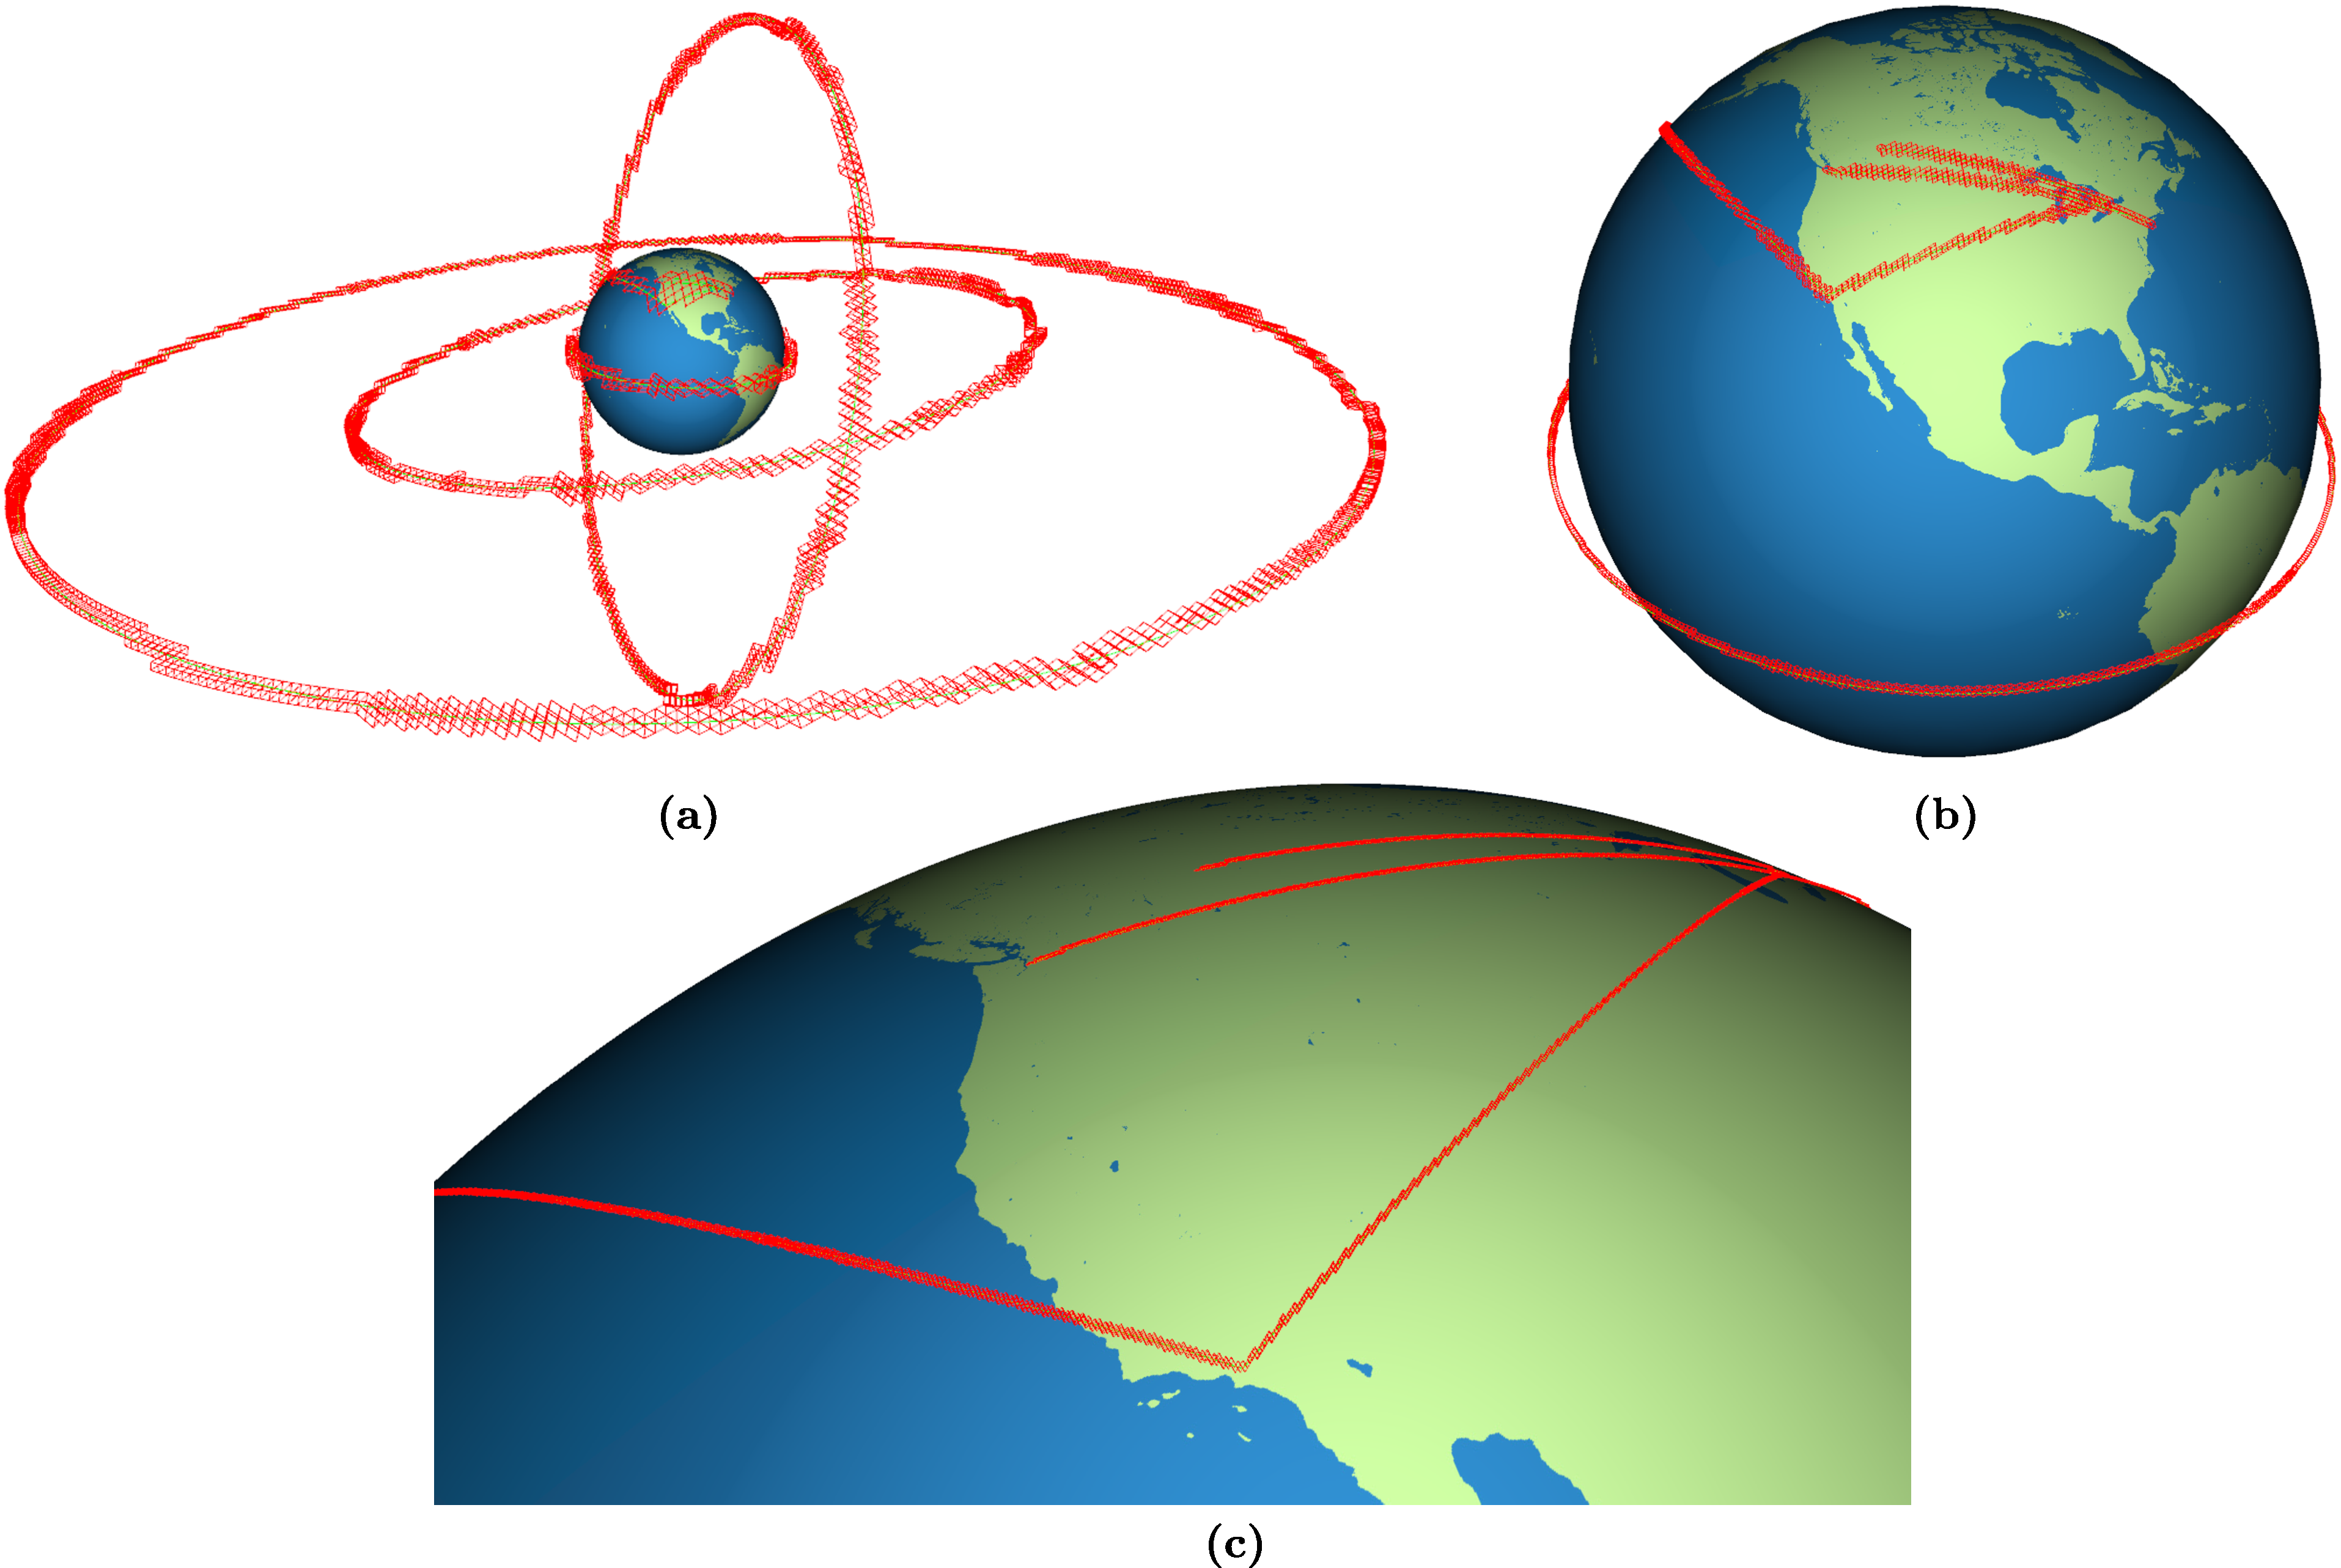
\includegraphics[width=\columnwidth]{sats.pdf}
	\caption{Flight paths and satellite orbits rasterized in a 3D DGGS.
		All paths and orbits are rasterized at the same grid resolution of \textbf{(a)} 7, \textbf{(b)} 10, and \textbf{(c)} 13}
	\label{fig:satellites}
\end{figure}


Figure~\ref{fig:satellites} shows several generated flight paths and satellite orbits represented in a 3D DGGS at increasing resolutions.
The input DGGS for this example uses a rhombic triacontahedron as the initial polyhedron, standard 1:4 quadrilateral refinement, and a simple normalization projection.
The 3D DGGS has a target aspect ratio of one, a radial mapping exponent of one, and a radial range of 10.66$R$ (67,957~km).
These parameters were chosen to ensure that cells are as compact as possible.

\section{Urban Planning}
The second use case is a volume-preserving 3D grid for the purpose of urban planning and management.
A volume-preserving grid is useful for quickly estimating the volume of a feature that has been rasterized in the grid by multiplying the number of cells by their volume.
This use case also shows the ability of our 3D DGGS to handle small scale data in addition to the much larger scale data showcased in the previous one.


\begin{figure}[h]
	\centering
	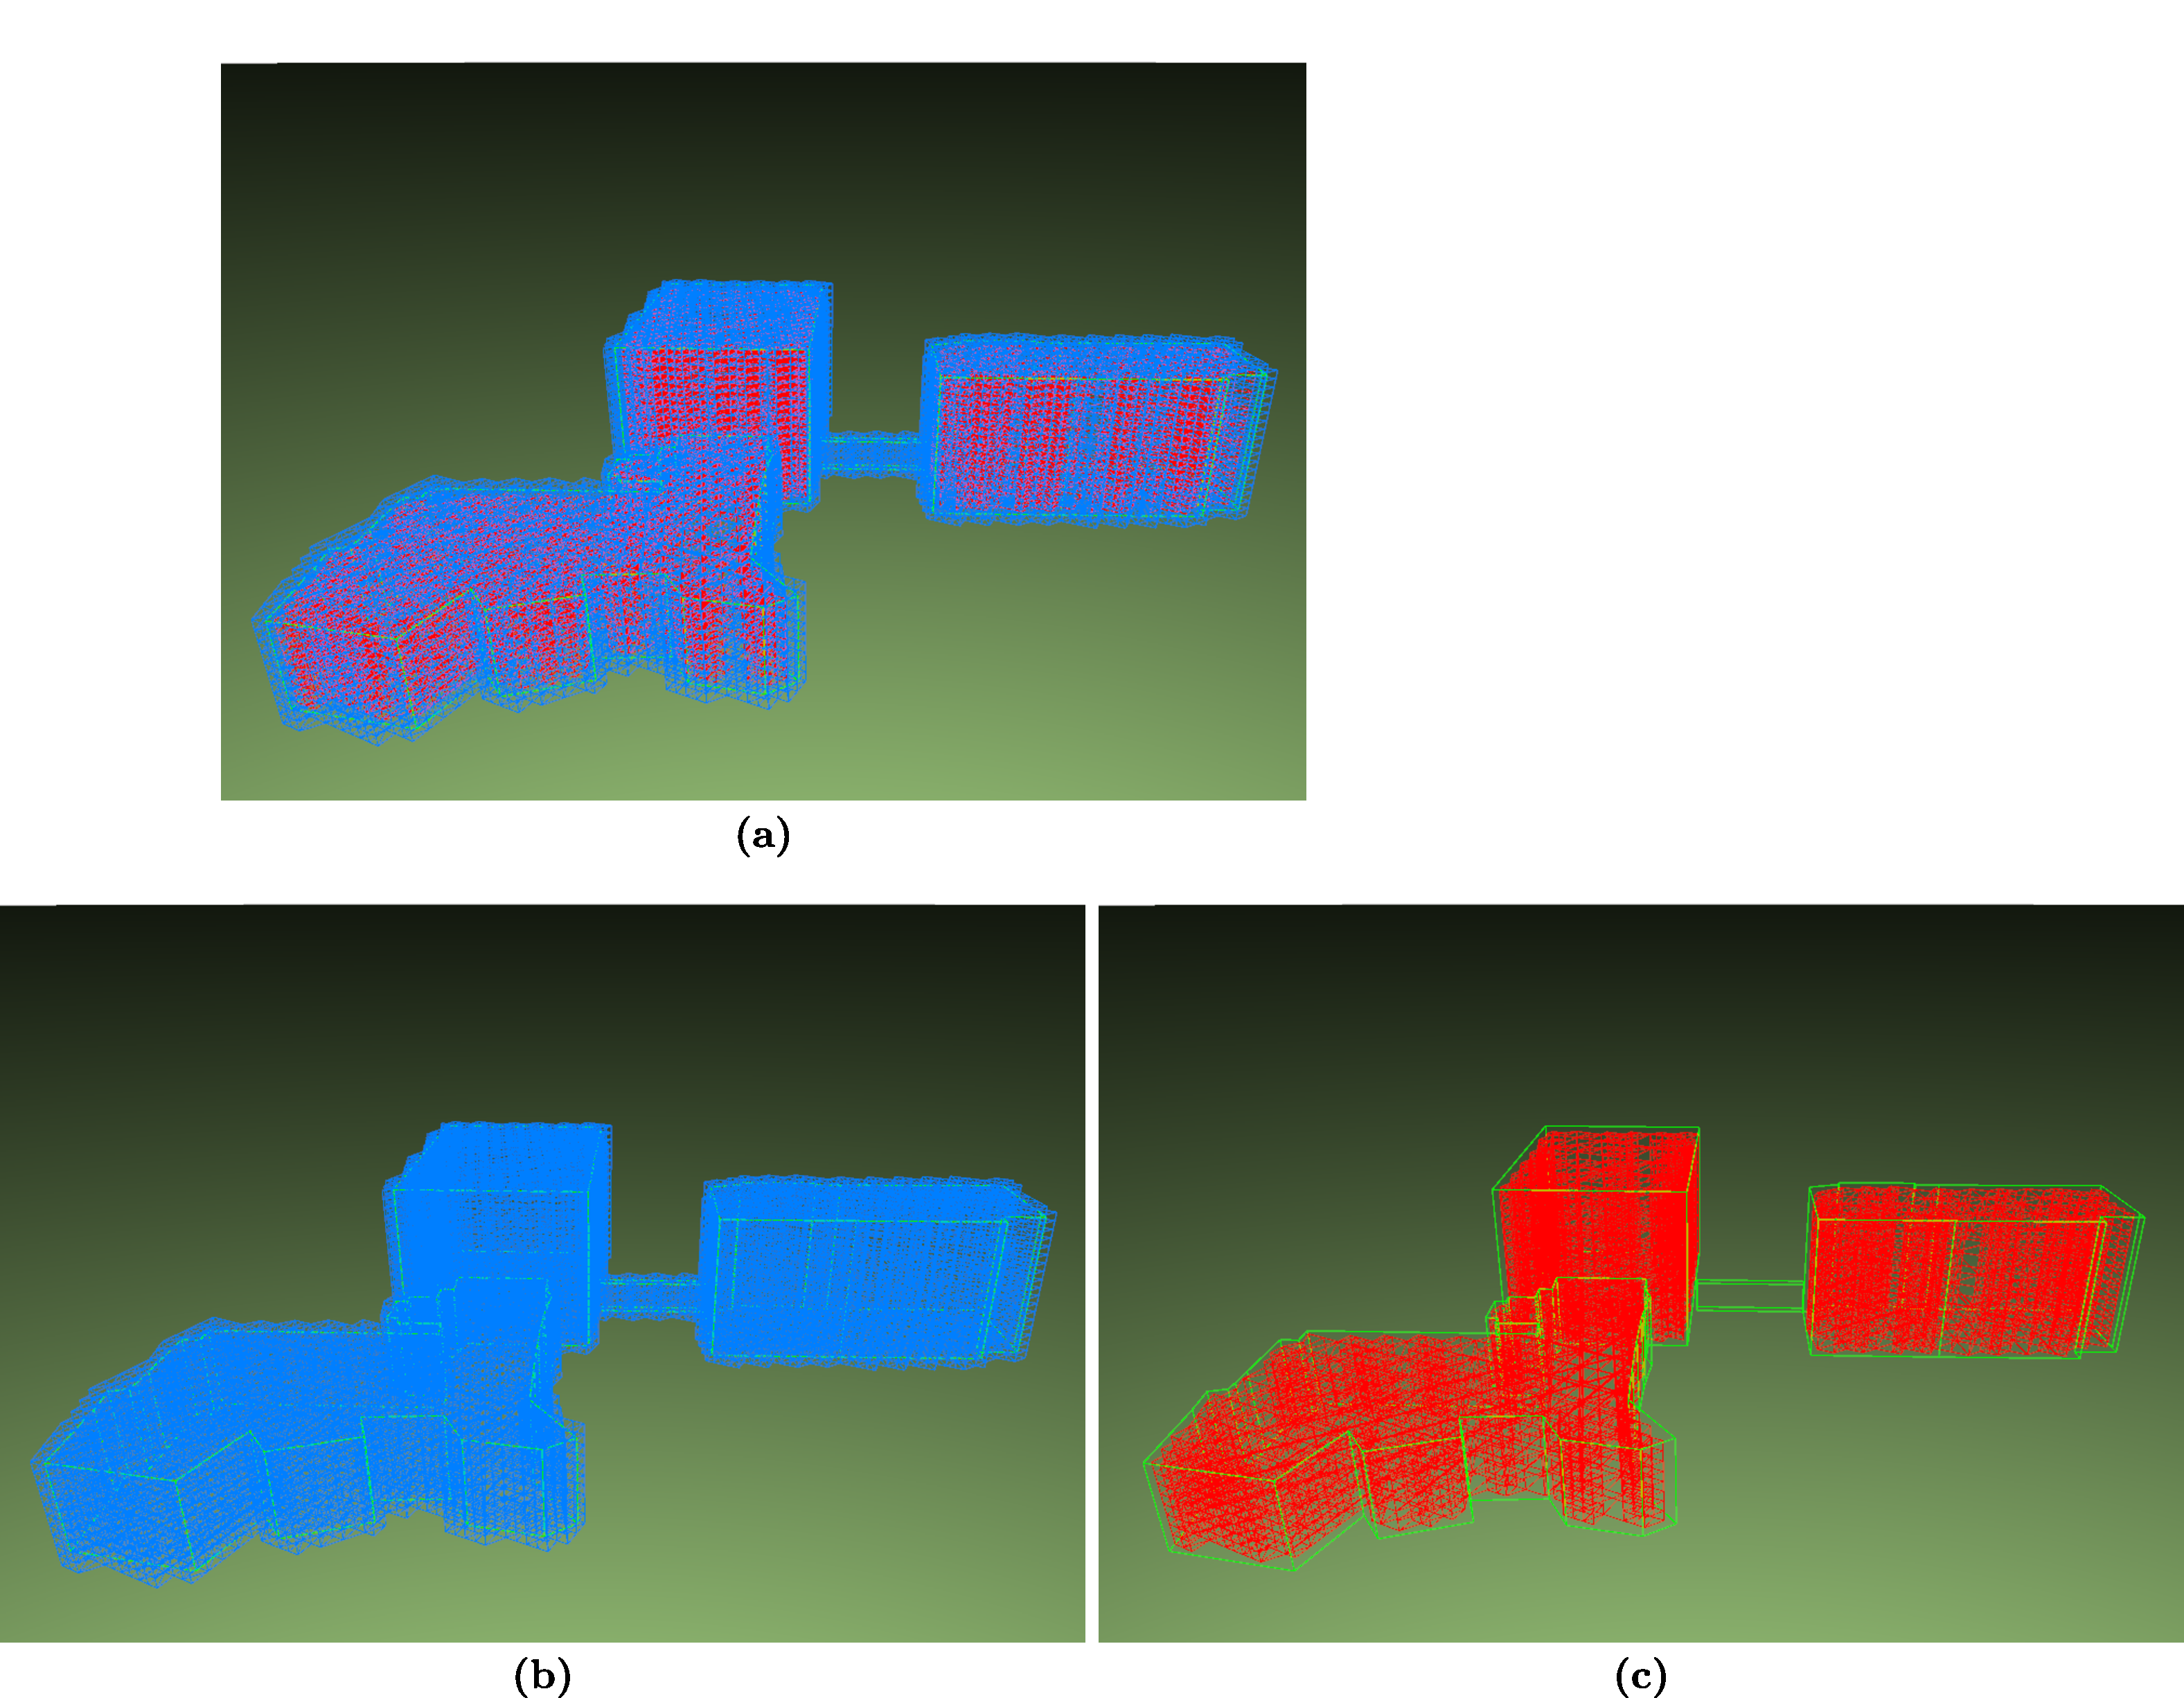
\includegraphics[width=\columnwidth]{builds.pdf}
	\caption{A collection of buildings from the University of Calgary rasterized in a 3D DGGS at resolution 21.
		In \textbf{(a)}, both interior and boundary cells are shown, whereas \textbf{(b)} and \textbf{(c)} show only boundary and interior cells, respectively}
	\label{fig:urbanplanning}
\end{figure}


Figure~\ref{fig:urbanplanning} shows several buildings represented in a 3D DGGS, with the building geometries obtained from Open Street Map\footnote{\url{www.openstreetmap.org}}.
The input DGGS for this example uses a disdyakis triacontahedron as the initial polyhedron, a non-standard 1:4 triangle refinement to maintain the relative shape of triangles, and the vertex oriented great circle slice and dice projection~\cite{van2006slice} to preserve area~\cite{hallDT}.
The 3D DGGS has a target aspect ratio of one, a radial mapping exponent of three to achieve perfect volume preservation (excluding the central layer), and a maximum radius of 1.33$R$ (8495~km).


\section{Atmospheric Properties}
The final use case we look at is using a 3D DGGS to resample atmospheric forecasts, such as those generated by numerical weather prediction models.
These datasets typically have a much higher vertical resolution than surface resolution, due to how quickly properties such as temperature and wind speed tend to change in these two dimensions.
To accommodate this with our 3D DGGS, we can specify an appropriate aspect ratio for cells to ensure the vertical and surface resolution matches as closely as possible that of the input data.


\begin{figure}[h]
	\centering
	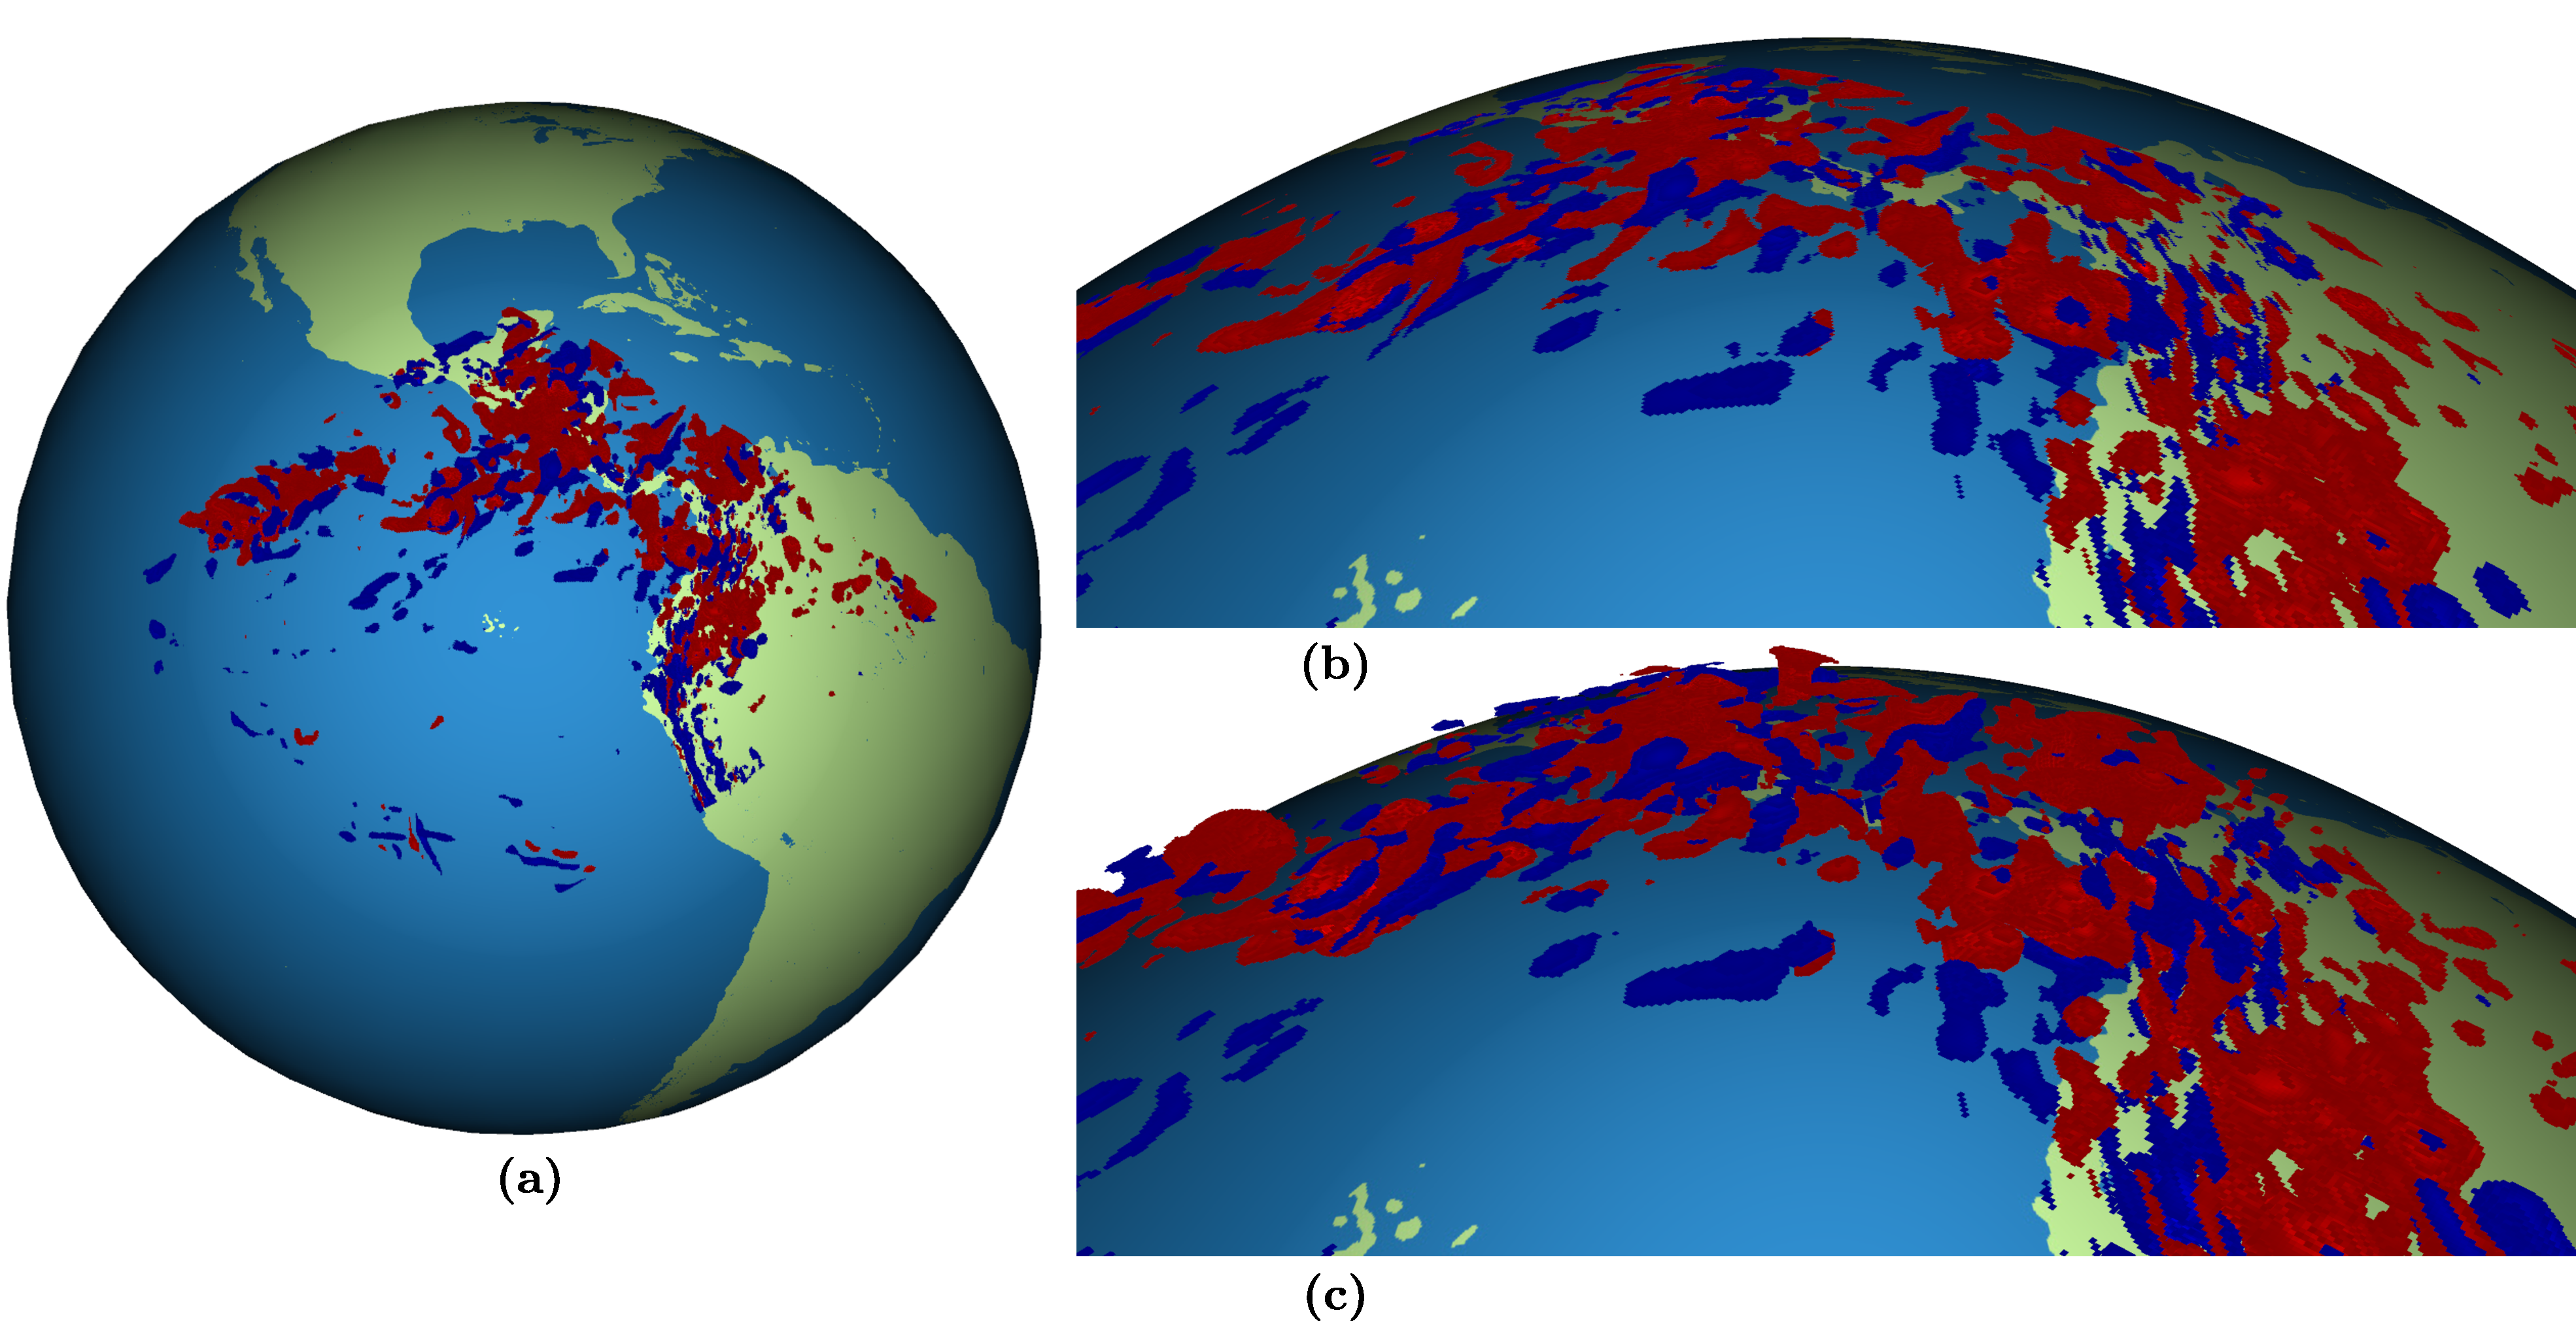
\includegraphics[width=\columnwidth]{atm.pdf}
	\caption{Vertical wind speed (mbar/s) sampled into a 3D DGGS at resolution 9.
		Negative velocity, which corresponds to an upward wind, is shown in red.
		Positive velocity, which corresponds to a downward wind, is shown in blue.
		Velocities with magnitude less than 0.25 mbars/s are not shown to reduce clutter and highlight regions with the highest speeds.
		In \textbf{(a)} and \textbf{(c)}, the altitude of cells is scaled by a factor of 15 to better show changes in altitude.
		In \textbf{(b)}, altitude is shown at its true scale}
	\label{fig:atmosphere}
\end{figure}


Figure~\ref{fig:atmosphere} shows vertical wind speed from the ERA5 dataset~\cite{era5} sampled into a 3D DGGS.
The input DGGS for this example is the same as the one used for the aircraft and satellite paths.
However, this 3D DGGS has a target aspect ratio of 31.7, a radial mapping exponent of one, and a maximum radius of 1.33$R$ (8495~km).


\subsection{Discussion}
The above examples are only a small subset of the many potential applications of our 3D DGGSs.
Despite this, they show not only the useful properties achievable by the method (support for large ranges of altitudes, volume preservation between cells, custom cell aspect ratio, and support for multiple scales of data) but also demonstrate the ease at which new 3D global grids can be created.
Given a conventional DGGS that provides the required operations, creating a 3D DGGS is as simple as providing the surface grid and four clearly defined parameters for the 3D one.
Since creating a 3D DGGS that is ideal for every application is not possible, this allows quick iterations on creating and comparing different 3D grids to find the ideal one for each application.
\chapter{Conclusion}

\section{Limitations and Future Work}
\section{Closing Remarks}
% end

\appendix
\chapter{First Appendix}

%Start the body text
Lorem ipson dolor sic amet sec in consetum epsom nunc ad valorem. Lorem ipson dolor sic amet
sec in consetum nunc ad valorem. Lorem epsom ipson dolor sic amet sec in consetum nunc ad valorem.
Lorem ipson dolor sic amet sec in consetum nunc ad valorem. Lorem ipson dolor sic amet
sec in consetum nunc ad valorem. Lorem ipson dolor sic amet sec in epsom consetum nunc ad valorem.

Lorem ipson dolor sic amet sec in consetum epsom nunc ad valorem. Lorem ipson dolor sic amet
sec in consetum nunc ad valorem. Lorem epsom ipson dolor sic amet sec in consetum nunc ad valorem.
Lorem ipson dolor sic amet sec in consetum nunc ad valorem. Lorem ipson dolor sic amet
sec in consetum nunc ad valorem. Lorem ipson dolor sic amet sec in epsom consetum nunc ad valorem.
Lorem ipson dolor sic amet sec in consetum epsom nunc ad valorem. Lorem ipson dolor sic amet
sec in consetum nunc ad valorem. Lorem epsom ipson dolor sic amet sec in consetum nunc ad valorem.
Lorem ipson dolor sic amet sec in consetum nunc ad valorem. Lorem ipson dolor sic amet
sec in consetum nunc ad valorem. Lorem ipson dolor sic amet sec in epsom consetum nunc ad valorem.
Lorem ipson dolor sic amet sec in consetum epsom nunc ad valorem. Lorem ipson dolor sic amet
sec in consetum nunc ad valorem. Lorem epsom ipson dolor sic amet sec in consetum nunc ad valorem.
Lorem ipson dolor sic amet sec in consetum nunc ad valorem. Lorem ipson dolor sic amet
sec in consetum nunc ad valorem. Lorem ipson dolor sic amet sec in epsom consetum nunc ad valorem.

Lorem ipson dolor sic amet sec in consetum epsom nunc ad valorem. Lorem ipson dolor sic amet
sec in consetum nunc ad valorem. Lorem epsom ipson dolor sic amet sec in consetum nunc ad valorem.
Lorem ipson dolor sic amet sec in consetum nunc ad valorem. Lorem ipson dolor sic amet
sec in consetum nunc ad valorem. Lorem ipson dolor sic amet sec in epsom consetum nunc ad valorem.
Lorem ipson dolor sic amet sec in consetum epsom nunc ad valorem. Lorem ipson dolor sic amet
sec in consetum nunc ad valorem. Lorem epsom ipson dolor sic amet sec in consetum nunc ad valorem.
Lorem ipson dolor sic amet sec in consetum nunc ad valorem. Lorem ipson dolor sic amet
sec in consetum nunc ad valorem. Lorem ipson dolor sic amet sec in epsom consetum nunc ad valorem.
\begin{figure}
Place the figure here
\caption{Figure in the appendix}
\end{figure}

Lorem ipson dolor sic amet sec in consetum epsom nunc ad valorem. Lorem ipson dolor sic amet
sec in consetum nunc ad valorem. Lorem epsom ipson dolor sic amet sec in consetum nunc ad valorem.
Lorem ipson dolor sic amet sec in consetum nunc ad valorem. Lorem ipson dolor sic amet
sec in consetum nunc ad valorem. Lorem ipson dolor sic amet sec in epsom consetum nunc ad valorem.
Lorem ipson dolor sic amet sec in consetum epsom nunc ad valorem. Lorem ipson dolor sic amet
sec in consetum nunc ad valorem. Lorem epsom ipson dolor sic amet sec in consetum nunc ad valorem.
Lorem ipson dolor sic amet sec in consetum nunc ad valorem. Lorem ipson dolor sic amet
sec in consetum nunc ad valorem. Lorem ipson dolor sic amet sec in epsom consetum nunc ad valorem.

Lorem ipson dolor sic amet sec in consetum epsom nunc ad valorem. Lorem ipson dolor sic amet
sec in consetum nunc ad valorem. Lorem epsom ipson dolor sic amet sec in consetum nunc ad valorem.
Lorem ipson dolor sic amet sec in consetum nunc ad valorem. Lorem ipson dolor sic amet
sec in consetum nunc ad valorem. Lorem ipson dolor sic amet sec in epsom consetum nunc ad valorem.
Lorem ipson dolor sic amet sec in consetum epsom nunc ad valorem. Lorem ipson dolor sic amet
sec in consetum nunc ad valorem. Lorem epsom ipson dolor sic amet sec in consetum nunc ad valorem.
Lorem ipson dolor sic amet sec in consetum nunc ad valorem. Lorem ipson dolor sic amet
sec in consetum nunc ad valorem. Lorem ipson dolor sic amet sec in epsom consetum nunc ad valorem.

Lorem ipson dolor sic amet sec in consetum epsom nunc ad valorem. Lorem ipson dolor sic amet
sec in consetum nunc ad valorem. Lorem epsom ipson dolor sic amet sec in consetum nunc ad valorem.
Lorem ipson dolor sic amet sec in consetum nunc ad valorem. Lorem ipson dolor sic amet
sec in consetum nunc ad valorem. Lorem ipson dolor sic amet sec in epsom consetum nunc ad valorem.
Lorem ipson dolor sic amet sec in consetum epsom nunc ad valorem. Lorem ipson dolor sic amet
sec in consetum nunc ad valorem. Lorem epsom ipson dolor sic amet sec in consetum nunc ad valorem.
Lorem ipson dolor sic amet sec in consetum nunc ad valorem. Lorem ipson dolor sic amet
sec in consetum nunc ad valorem. Lorem ipson dolor sic amet sec in epsom consetum nunc ad valorem.
\begin{table}
\caption{Table in the appendix}
\center{Place the table here}
\end{table}
Lorem ipson dolor sic amet sec in consetum epsom nunc ad valorem. Lorem ipson dolor sic amet
sec in consetum nunc ad valorem. Lorem epsom ipson dolor sic amet sec in consetum nunc ad valorem.
Lorem ipson dolor sic amet sec in consetum nunc ad valorem. Lorem ipson dolor sic amet
sec in consetum nunc ad valorem. Lorem ipson dolor sic amet sec in epsom consetum nunc ad valorem.
Lorem ipson dolor sic amet sec in consetum epsom nunc ad valorem. Lorem ipson dolor sic amet
sec in consetum nunc ad valorem. Lorem epsom ipson dolor sic amet sec in consetum nunc ad valorem.
Lorem ipson dolor sic amet sec in consetum nunc ad valorem. Lorem ipson dolor sic amet
sec in consetum nunc ad valorem. Lorem ipson dolor sic amet sec in epsom consetum nunc ad valorem.

Lorem ipson dolor sic amet sec in consetum epsom nunc ad valorem. Lorem ipson dolor sic amet
sec in consetum nunc ad valorem. Lorem epsom ipson dolor sic amet sec in consetum nunc ad valorem.
Lorem ipson dolor sic amet sec in consetum nunc ad valorem. Lorem ipson dolor sic amet
sec in consetum nunc ad valorem. Lorem ipson dolor sic amet sec in epsom consetum nunc ad valorem.
Lorem ipson dolor sic amet sec in consetum epsom nunc ad valorem. Lorem ipson dolor sic amet
sec in consetum nunc ad valorem. Lorem epsom ipson dolor sic amet sec in consetum nunc ad valorem.
Lorem ipson dolor sic amet sec in consetum nunc ad valorem. Lorem ipson dolor sic amet
sec in consetum nunc ad valorem. Lorem ipson dolor sic amet sec in epsom consetum nunc ad valorem.


Lorem ipson dolor sic amet sec in consetum epsom nunc ad valorem. Lorem ipson dolor sic amet
sec in consetum nunc ad valorem. Lorem epsom ipson dolor sic amet sec in consetum nunc ad valorem.
Lorem ipson dolor sic amet sec in consetum nunc ad valorem. Lorem ipson dolor sic amet
sec in consetum nunc ad valorem. Lorem ipson dolor sic amet sec in epsom consetum nunc ad valorem.
Lorem ipson dolor sic amet sec in consetum epsom nunc ad valorem. Lorem ipson dolor sic amet
sec in consetum nunc ad valorem. Lorem epsom ipson dolor sic amet sec in consetum nunc ad valorem.
Lorem ipson dolor sic amet sec in consetum nunc ad valorem. Lorem ipson dolor sic amet
sec in consetum nunc ad valorem. Lorem ipson dolor sic amet sec in epsom consetum nunc ad valorem.




\bibliographystyle{acm}
\nocite{*}
\bibliography{sources}

\end{document}
